\chapter{FSK変調方式による電力・データ同時伝送システム}
\section{原理ならびに構成}
2.2節において述べたとおり,極大電力周波数の近傍にあるZRFは2つ存在し,それらの周波数における出力電力$P_{ZRF}$は等しい.したがって,2値のデータを各ZRFに割り当てることにより,データによる出力電力の変動を避けながら,電力とデータの同時伝送(Simultaneous Wireless Information and Power Transfer : SWIPT)が実現できると考えられる.これは,2値データに対応させて電力伝送に用いる交番磁界の周波数を切り替える,すなわち周波数偏移(Frequency Shift Keying : FSK)変調を行うことと同義である.実際にこの動作を行うためには,図\ref{concept}のように,$f_{ZRF1}$あるいは$f_{ZRF2}$のいずれかのみにロックするPLLを用意し,データに対応させてそれらの出力を選択すればよい.

\begin{figure}[b]
\begin{center}

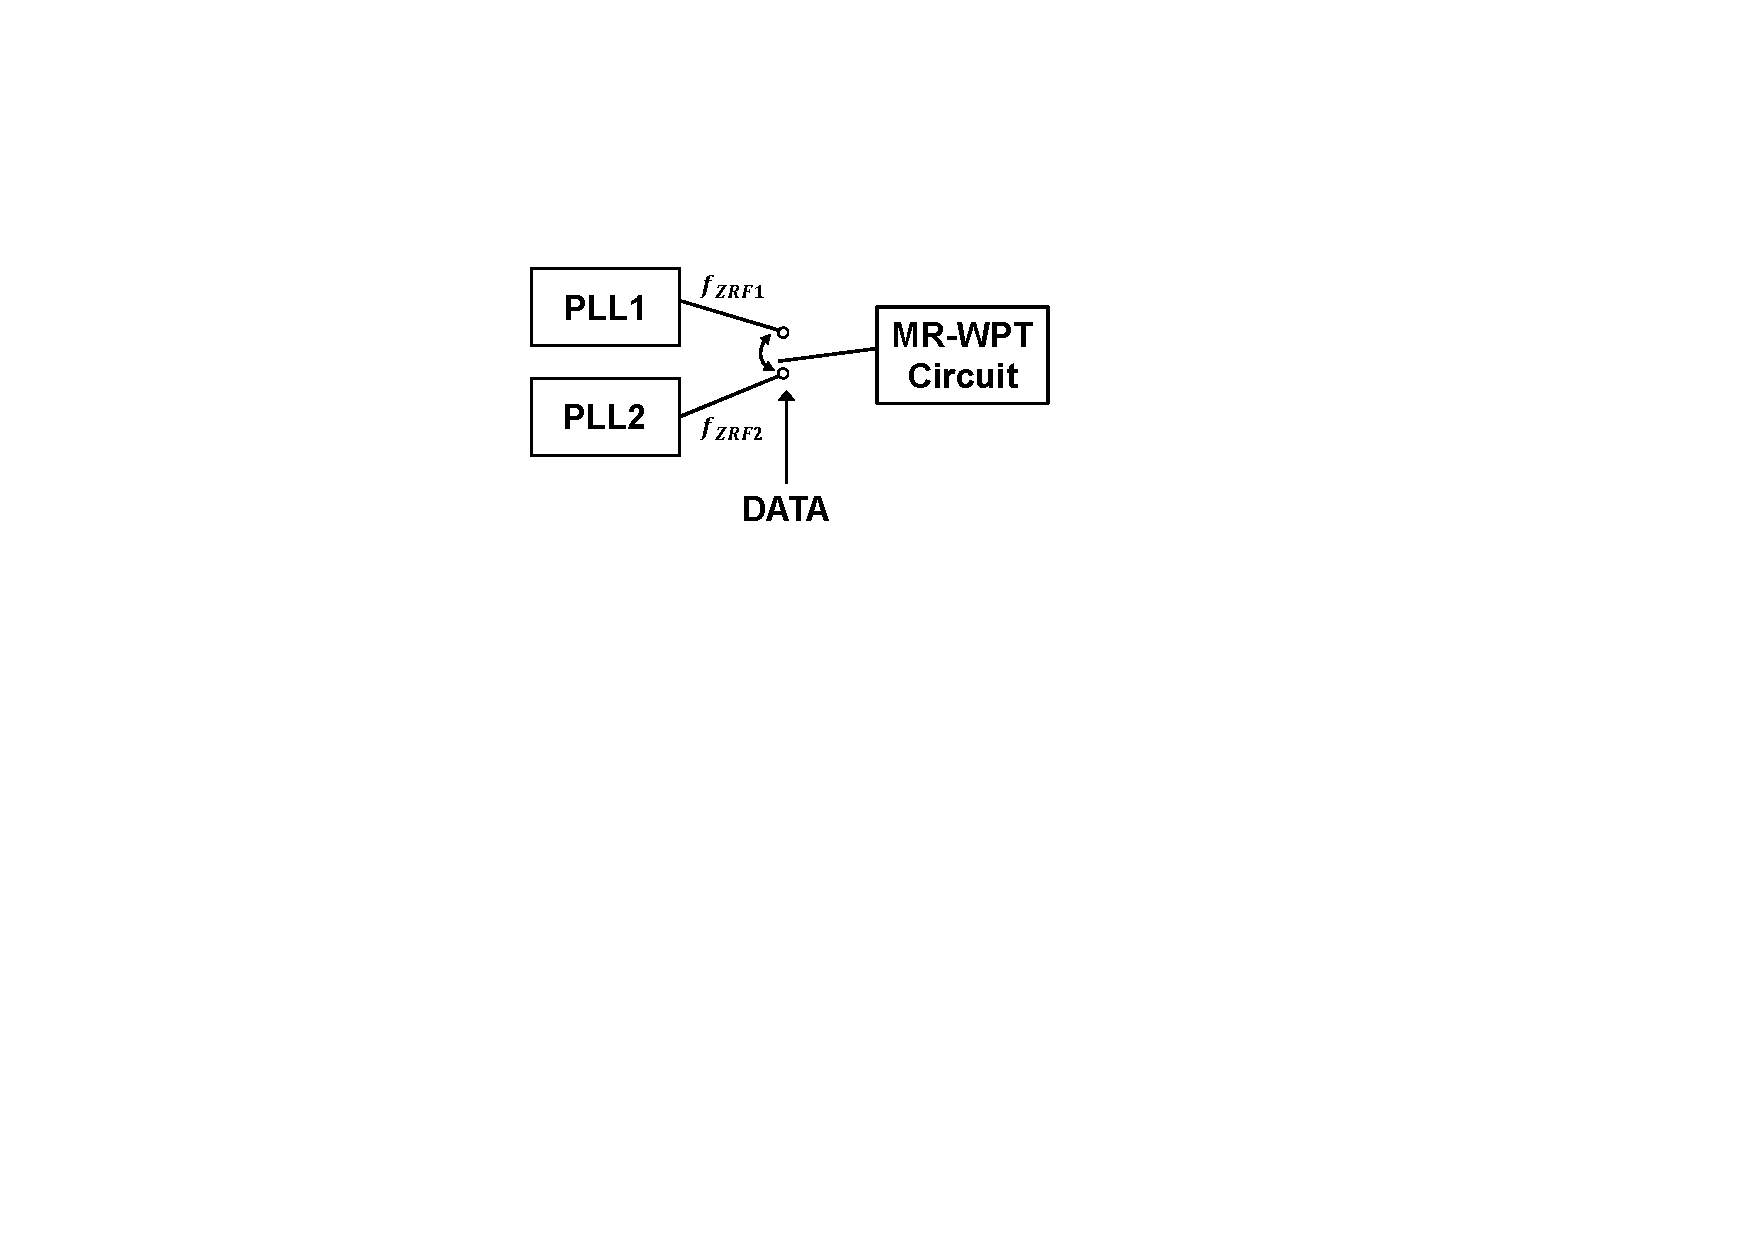
\includegraphics[width=80mm]{figures/concept.pdf}
\caption{FSK変調方式による電力・データ同時伝送システムの概念図}
\label{concept}
\end{center}

\end{figure}

図\ref{concept}の構成でFSK変調を実現するためには,各PLLがノイズや回路の初期状態によらず常に同じZRFにロックしている必要がある.図\ref{entireblock}の回路においては,PLLが複数あるうちのいずれのZRFにロックするかは考慮されておらず,上述した要因によりロックする周波数が変動してしまう問題があった.この問題を避けるためには,何らかの方法によりVCOの出力周波数範囲を制限すればよい.例えば,図\ref{entireblock}において用いているPLL-IC CD74HC4046A(Texas Instruments)では,2つの外付け抵抗によりVCOの出力周波数範囲を設定することができる\cite{4046}.極大電力周波数の近傍にあるZRF$f_{ZRF1}, f_{ZRF2}$の範囲は,MR-WPT回路をあらかじめ数値計算することにより求められるから,$f_{ZRF1}$のみを追従する回路,あるいは$f_{ZRF2}$のみを追従する回路をそれぞれ構成することができる.\par
図\ref{fskentirecircuit}に,提案するFSK変調方式による電力・データ同時伝送(FSK-SWIPT)システムの全体構成を示す.送電側は,図\ref{entireblock}におけるPLLをFSK変調器に置き換えた構成である.また受電側は,負荷抵抗$R_L$に直流出力電圧$V_{OUT}$を供給するためのブリッジダイオードによる全波整流回路と,リミタ回路,コンパレータを用いた波形整形回路ならびに復調用のFPGAから成る.変復調回路の詳細については後述する.

\begin{figure}[h]
\begin{center}

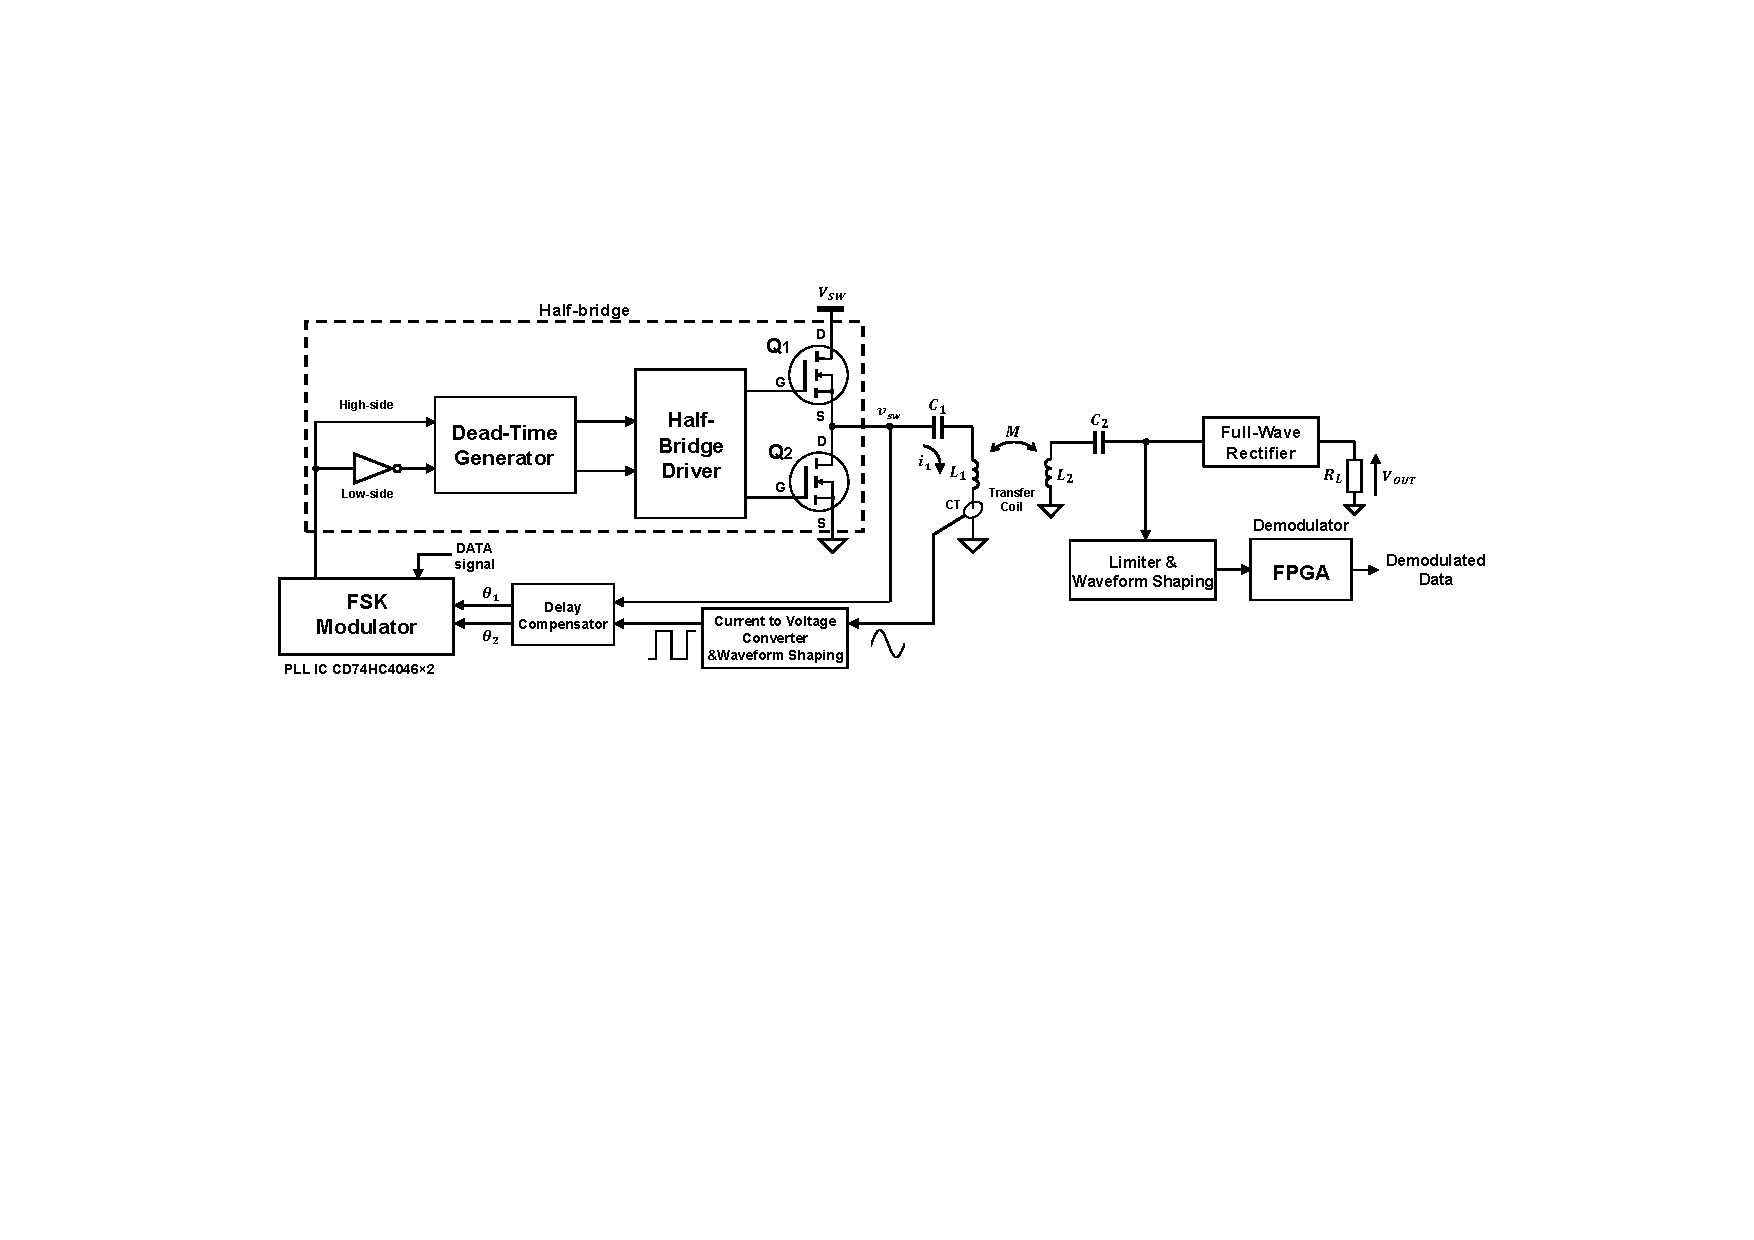
\includegraphics[width=160mm]{figures/fskentirecircuit.pdf}
\caption{FSK-SWIPTシステムの全体構成図}
\label{fskentirecircuit}
\end{center}

\end{figure}

\section{FSK変調回路}
\subsection{全体構成}
図\ref{fskmodulator}に,設計したFSK変調回路の全体構成を示す.同回路は,PFD1,LPF1,ならびにVCO1から成り$f_{ZRF1}$にロックするPLL1と,同様の構成で$f_{ZRF2}$にロックするPLL2を主体として構成されている.これらの回路の出力を,マルチプレクサによりデータ信号に対応させて切り替えることによりFSK変調を行う.また,補助的な回路として,タイミング制御回路(Timing Controller),ロック検出回路(Lock Detector)ならびに電圧制限回路(Voltage Restrictor)を付加している.以下,順に述べる.

\begin{figure}[h]
\begin{center}

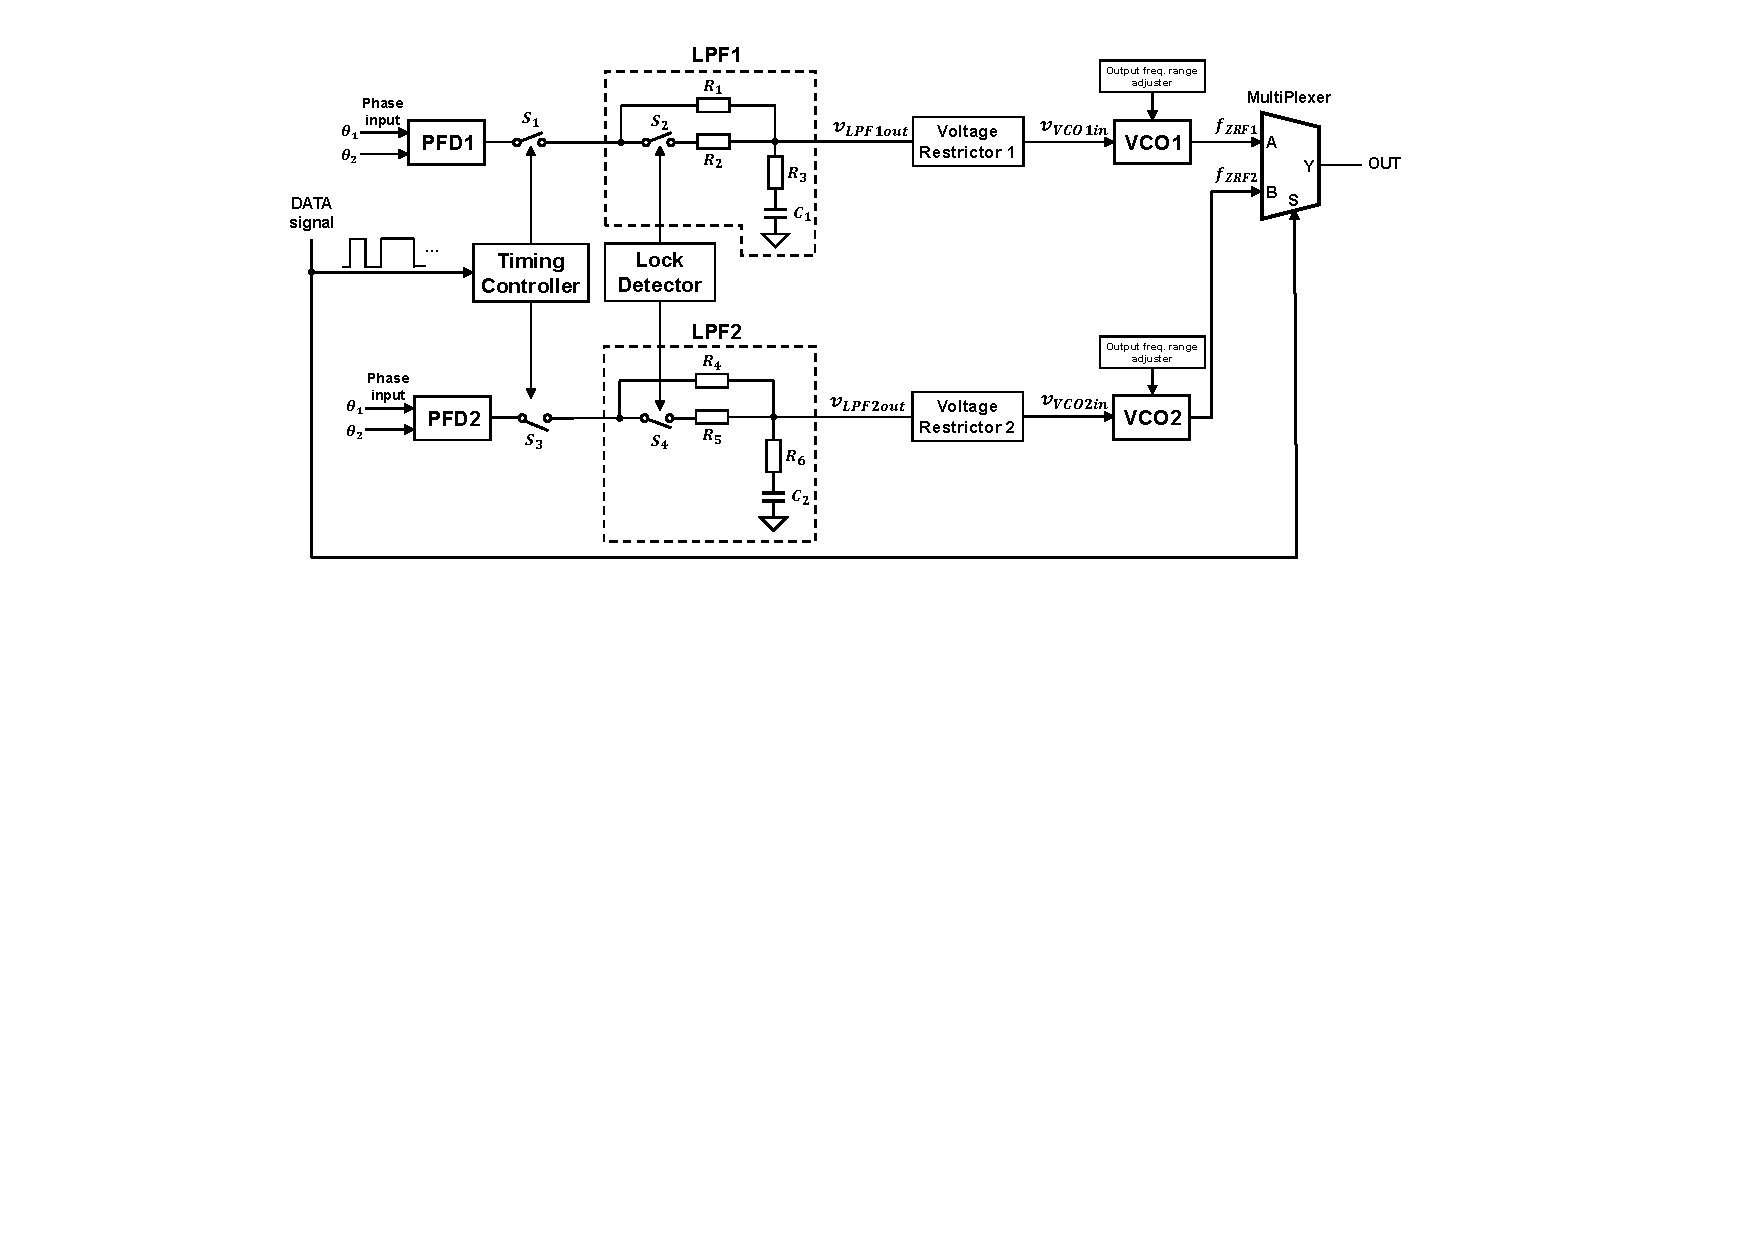
\includegraphics[width=160mm]{figures/fskmodulator.pdf}
\caption{FSK変調回路}
\label{fskmodulator}
\end{center}

\end{figure}

\subsection{内部回路}
\subsubsection{タイミング制御回路}
MR-WPT回路がZRFで駆動されているとき,LC共振回路のスイッチング特性から,回路を流れる電流$i_1$は正弦波状になる.3.2節において述べたとおり,$i_1$はコンパレータにより矩形波電圧信号に変換され,$i_1$が正弦波状であればそのDuty比はほぼ50\%になる.一方,MR-WPT回路がZRFでない周波数で駆動されているとき,$i_1$は正弦波状ではなくなるため,矩形波電圧信号のDuty比も不規則に変化する.このような信号をPFDに入力した場合,適切な位相比較が行えず,その出力が不安定になる.\par
提案手法によりFSK変調を行う場合,データの遷移に対応して回路を駆動する周波数を切り替える.周波数を切り替えるとき,電流$i_{1}$の周波数$f$は,過渡的に2つのZRFの間の周波数($f_{ZRF1}<f<f_{ZRF2}$)となる.このとき,先述した理由により,PFDの出力が不安定になり,ひいてはVCOの出力も不安定な状態となる.これを避けるためには,データの遷移時にPFDの出力を遮断すれば良い.このような動作を実現するために,タイミング制御回路を挿入する.PFDの出力が遮断されているとき,各VCOの制御電圧はキャパシタ$C_1,C_2$により一定に保持される.\par 
また,タイミング制御回路は,上記の動作に加え,MR-WPT回路がいずれかのPLLの出力で駆動されているとき他方のPLL中のPFD出力を遮断するよう動作する.例えば,MR-WPT回路がPLL1で駆動されているとき,PFD2の出力は遮断される.これは,各PLLを独立して動作させることで,ロック時間の短縮やループの安定化を図るためである.\par 
すなわち,タイミング制御回路は,データに対応して図\ref{fskmodulator}における電圧制御スイッチ$S_1, S_3$を開閉するとともに,データの遷移時には両方のスイッチを開放するような動作をする.これは,3.2.2節で述べた,スイッチング信号の遷移時にハーフブリッジにおける2つのFETをいずれもターンオフさせる,デッドタイム生成回路と全く同じ動作である.よって,回路構成は図\ref{deadtimegenerator}と同一のものであり,同図における「VCO output sig.」を「DATA signal」に,「High/Low-side drive sig.」をスイッチ$S_1, S_3$の開閉信号にそれぞれ読み替えれば良い.

\subsubsection{ロック検出回路}
PLLのロック時間とVCOの位相雑音特性は,LPFの時定数$\tau$に大きく依存する.ロック時間を短くしたい場合は$\tau$を小さくすればよいが,その場合LPFの遮断周波数が高くなってしまうため,PFDの出力パルスの高調波成分を十分に除去することができず,結果としてVCOの出力位相雑音が増大する.したがって,一般にロック時間と位相雑音とはトレードオフの関係にある.これを改善するためには,入力信号の位相差$|\theta_1-\theta_2|$が大きい,すなわちPLLがロック状態から遠いときは$\tau$を小さく,$|\theta_1-\theta_2|$が小さいときは$\tau$を大きくすればよい.\par 
Lock Detector回路は,入力信号の位相差$|\theta_1-\theta_2|$があるしきい値$\theta_t$より大きいか否かを判定し,図\ref{fskmodulator}における各LPF中にあるスイッチ$S_2,S_4$を制御する回路である.図\ref{lockdetector}のように,PFDで2信号の位相差を検出し,その平均電圧と基準電圧$V_{REF}$とを比較して$S_2,S_4$を開閉する.$\theta_t$は$V_{REF}$ならびに$R$を可変することで実験的に調整する.各スイッチが閉じているときは,開いているときよりも$\tau$が小さくなる.この回路を用いることで,ロック時間を短縮し,また外来ノイズ等による突発的なロック外れを抑制する.

\begin{figure}[h]
\begin{center}

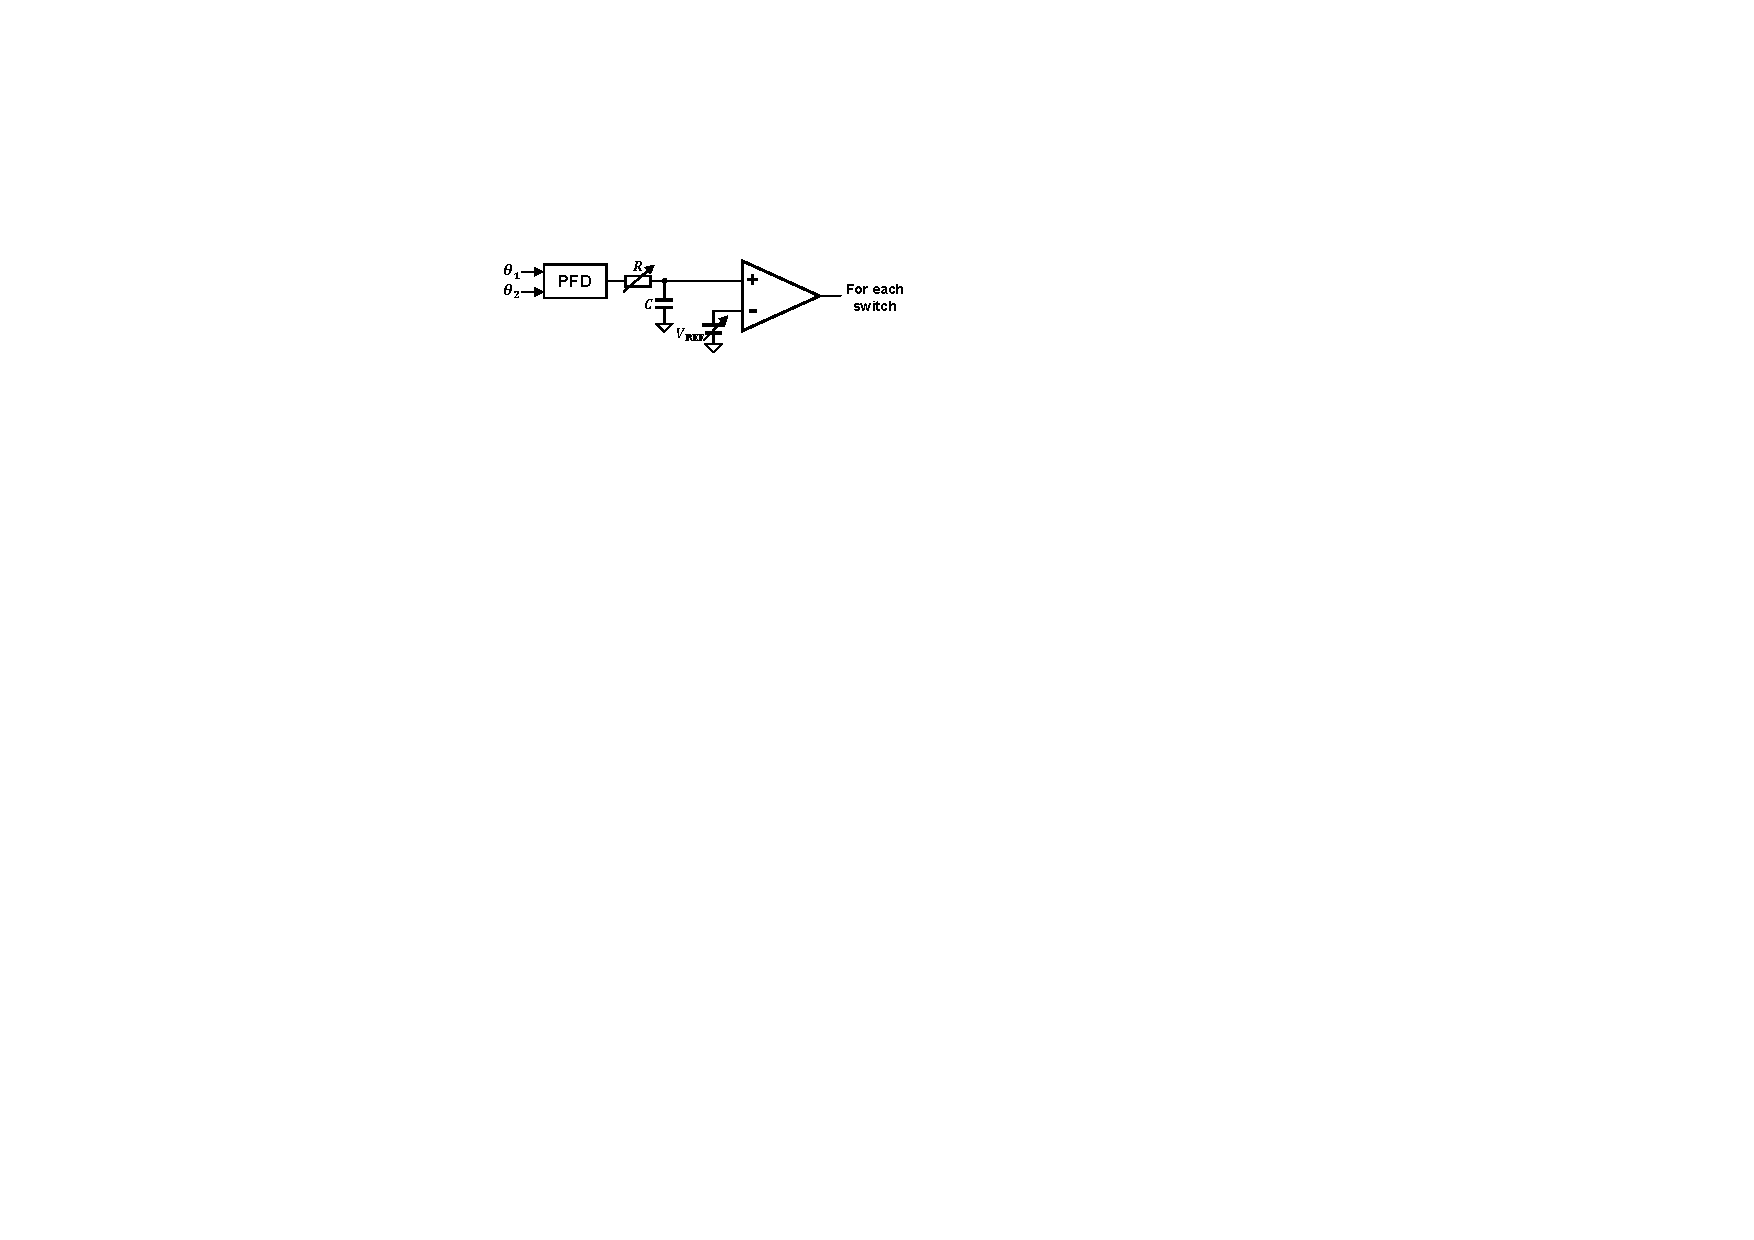
\includegraphics[width=120mm]{figures/lockdetector.pdf}
\caption{ロック検出回路}
\label{lockdetector}
\end{center}

\end{figure}

\subsubsection{電圧制限回路}
図\ref{fskentirecircuit}の回路で用いているPLL-IC  CD74HC4046(Texas Instruments)のVCOは,制御電圧-発振周波数特性がほぼ線形である領域と,指数関数的に非線形に変化する領域とが存在する.具体的には,ICを電源電圧$5 \, \mathrm{V}$で使用した場合,制御電圧がおよそ$1-4 \, \mathrm{V}$程度の範囲で制御電圧-発振周波数特性はほぼ線形となる\cite{Enzaka2014}.図\ref{fskentirecircuit}の回路では,FSK変調のためにVCOの発振周波数を適切に制限しなければならず,したがってVCOの制御電圧-発振周波数特性がほぼ線形である領域でVCOを駆動する必要がある.\par 
図\ref{voltagerestrictor}は,$0-V_{DD} \, \mathrm{[V]}$の値をとるLPFの出力電圧$v_{LPFout}$に対して,
\begin{eqnarray}
v_{vcoin}=\left\{ \begin{array}{ll}
v_y & (v_{LPFout}>v_y) \\
v_{LPFout} & (v_x<v_{LPFout}<v_y) \\
v_x & v_{LPFout}<v_x \\
\end{array} \right.
\end{eqnarray}
のように$v_x<v_{vcoin}<v_y$の範囲に制限されたVCOの制御電圧$v_{vcoin}$を出力する回路である.ここで,ダイオードは理想素子として扱っている.例えば,$v_{LPFout}>v_y$のとき,ダイオード$D_2$が導通するから,$v_{vcoin}$の上限は$v_y$に制限される.同様にして,$v_{LPFout}$の下限も$v_x$の制限される.実際は,$v_{vcoin}$の上限値と下限値はダイオード$D_1, \, D_2$の順方向電圧降下等に影響されるため,それらの値は$R_2$ならびに$R_3$を可変することにより実験的に調整する.


\begin{figure}[b]
\begin{center}

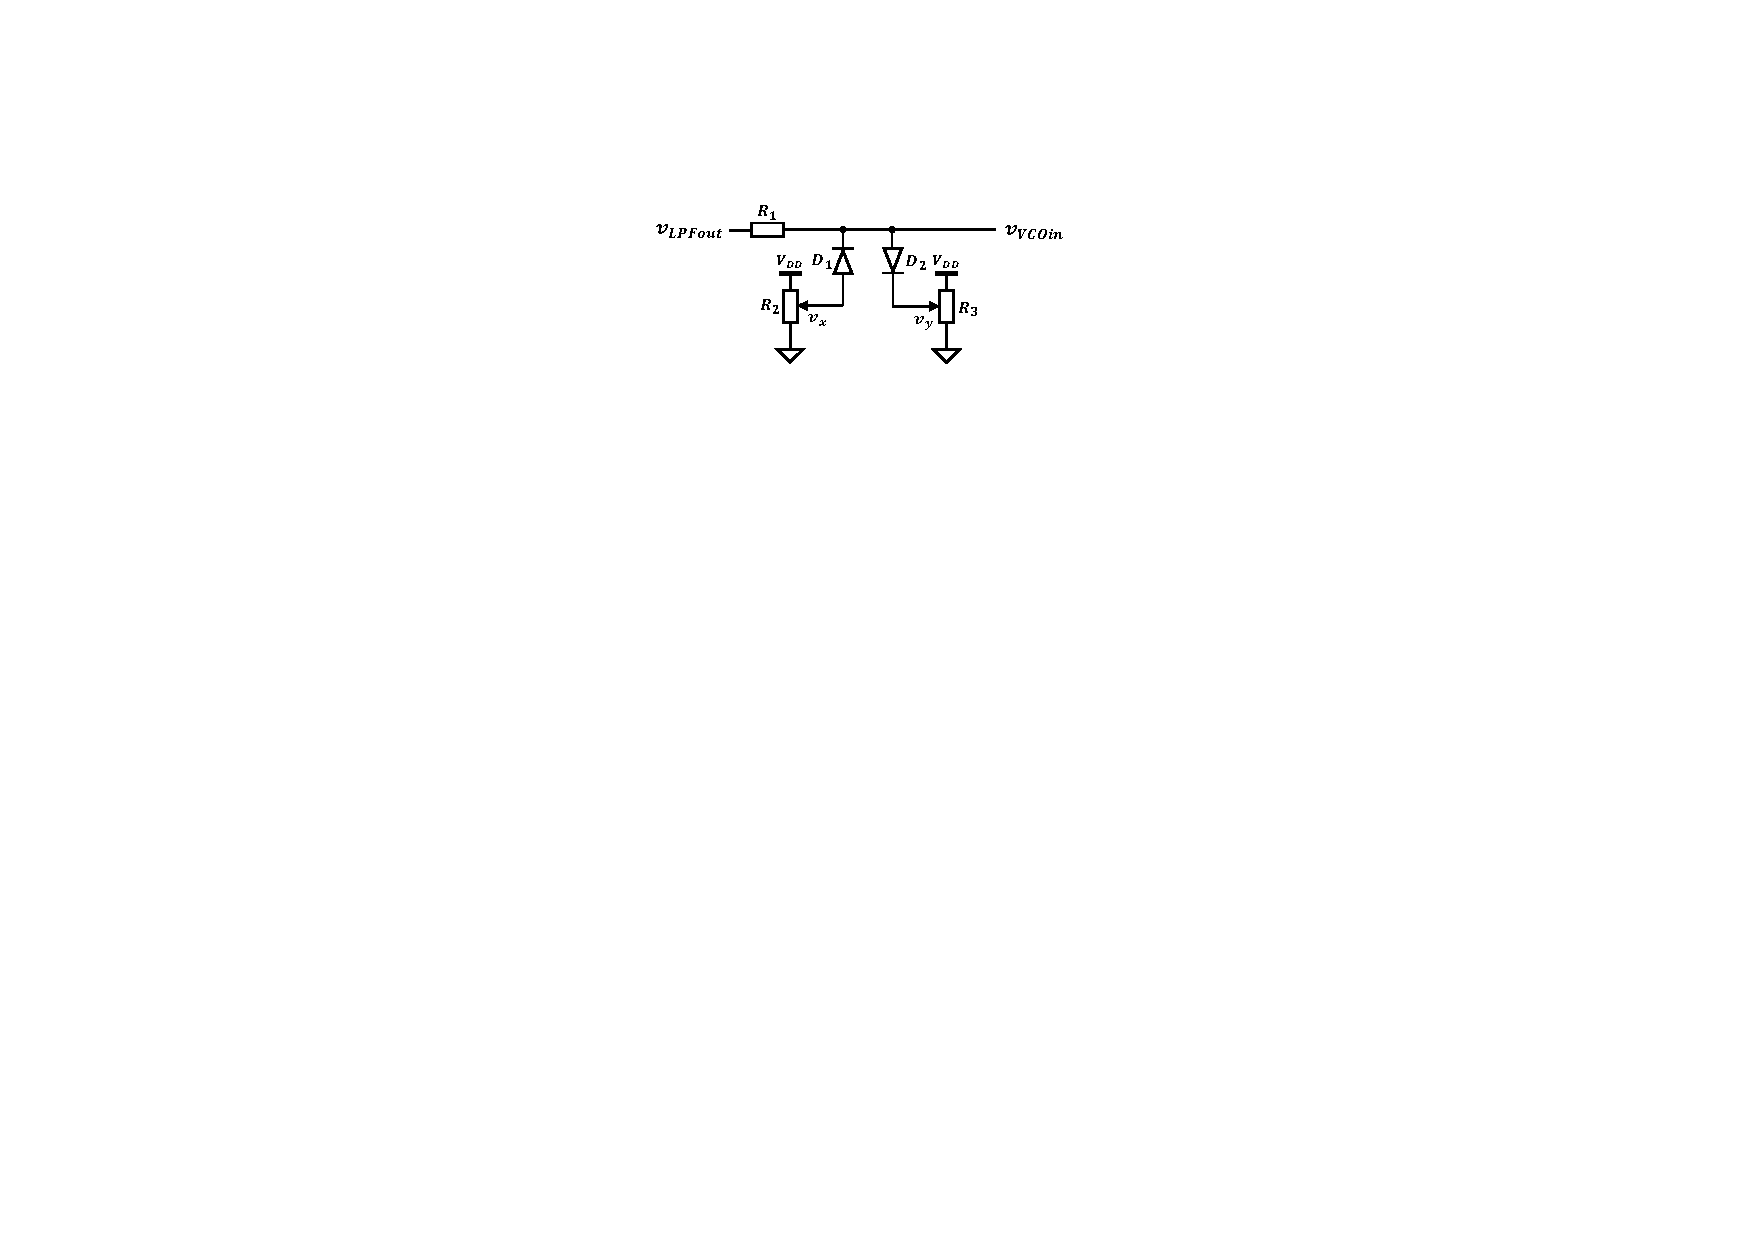
\includegraphics[width=110mm]{figures/voltagerestrictor.pdf}
\caption{電圧制限回路}
\label{voltagerestrictor}
\end{center}

\end{figure}


\section{シミュレーション}

図\ref{fskentirecircuit}ならびに図\ref{fskmodulator}の回路について,LTspiceでシミュレーションを行った.シミュレーション回路を図\ref{fsksimulationcircuit}に示す.ここで,伝送部のパラメータは表1のとおりとし,データ信号は周波数$5 \, \mathrm{kHz}$,Duty比0.5の矩形波(0101…の連続信号)とした.また,VCO,電圧制御スイッチとバッファには理想素子を用い,受信側の整流回路は等価的な負荷抵抗$R_{L}=5 \, \mathrm{\Omega}$に置換し,FPGAによる復調回路は省略した.さらに,PFDならびにハーフブリッジ回路は図\ref{pllsimulationcircuit}と同様の構成のものをサブサーキット化している.\par 

図\ref{fsksimulationcircuit}におけるVCO1, VCO2は,$0-1 \, \mathrm{V}$の制御電圧に対して1次関数で表される周波数を出力する理想VCOであり,出力周波数範囲はそれぞれ$500-700 \, \mathrm{kHz}$, $730-1100 \, \mathrm{kHz}$に設定してある.したがって,各VCOの制御電圧$v_{vcoin1}$,$v_{vcoin2} \, \mathrm{[V]}$と出力周波数$f_{vcoin1}$,$f_{vcoin2} \, \mathrm{[kHz]}$の関係は,
\begin{align}
f_{vcoin1} &=500+200\cdot v_{vcoin1} \\
f_{vcoin2} &=730+370\cdot v_{vcoin2}
\end{align}
\begin{figure}[H]
\begin{center}

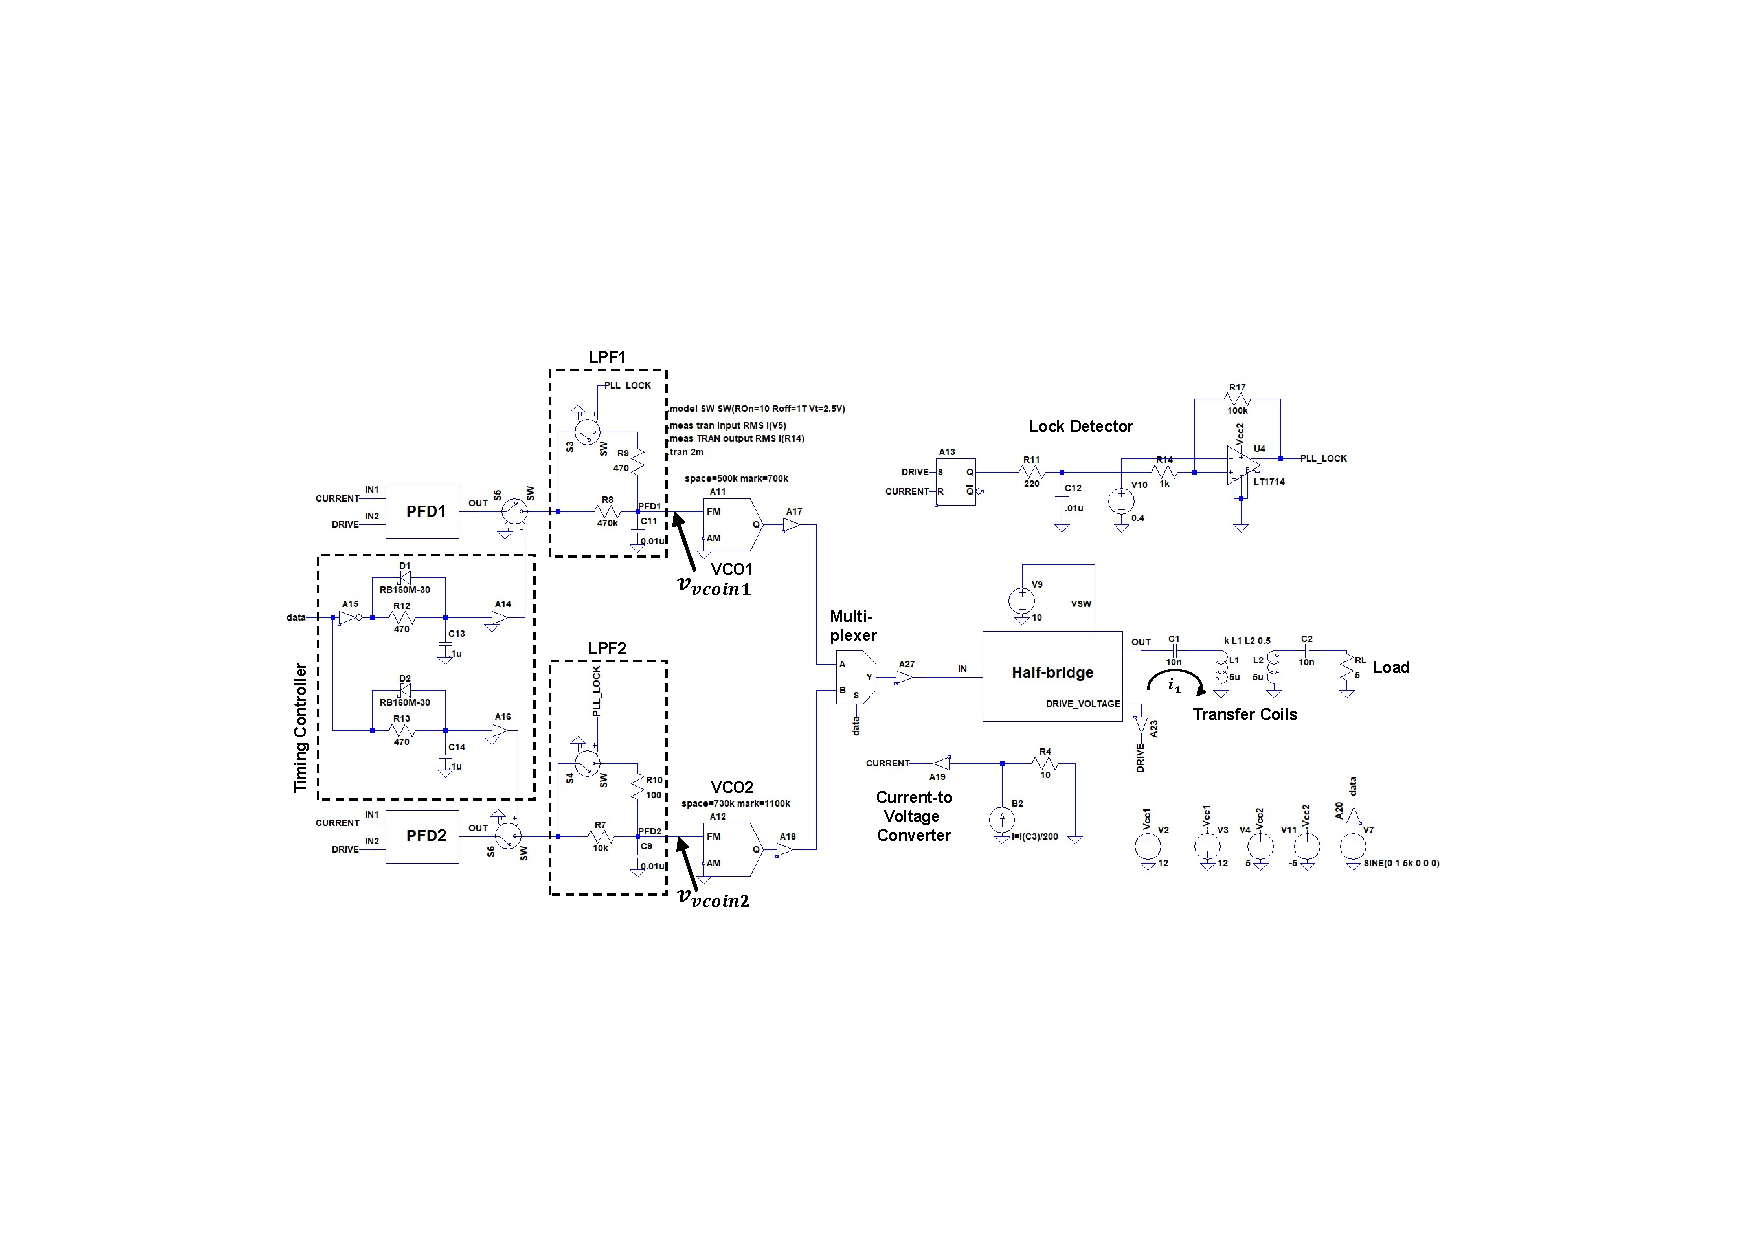
\includegraphics[width=155mm]{figures/fsksimulationcircuit.pdf}
\caption{FSK-SWIPTシステムのシミュレーション回路}
\label{fsksimulationcircuit}
\end{center}

\end{figure}
で表される.2つのZRFの周波数の理論値は,式(2.17),(2.18)から,$f_{ZRF1} \simeq 597\mathrm{kHz}, \, f_{ZRF2} \simeq 979 \mathrm{kHz}$であり,それらに対応するVCO1, VCO2の制御電圧$v_{vcoin1}, \, v_{vcoin2}$は,式(4.2),(4.3)より$v_{vcoin1}\simeq 0.49, \, v_{vcoin2} \simeq 0.67 \, \mathrm{V}$である.図\ref{fsksimulationgraph1}に,$v_{vcoin1}, \, v_{vcoin2}$の過渡解析結果を示す.同図から明らかなように,VCOの制御電圧はほぼ理論値付近にロックしている.データ信号の周期は$0.2 \, \mathrm{ms}$,シミュレーション時間は$1 \, \mathrm{ms}$であるから,データの値によらず安定した制御電圧が得られている.\par
図\ref{fsksimulationgraph2}は,データ信号ならび負荷抵抗$R_L$の電流の過渡解析結果である.定常状態においては,データによらず負荷電流の振幅はほぼ等しくなっている.また,データのHIGHとLOWに対応して周波数が変化している.図\ref{fsksimulationgraph3}は,電流$i_1$の過渡解析結果をFFT解析することにより得られたスペクトルである.2つのZRFの理論値$f_{ZRF1} \simeq 597\mathrm{kHz}, \, f_{ZRF2} \simeq 979 \mathrm{kHz}$付近にスペクトルのピークがあり,シミュレーション回路が所望の動作を実現できているといえる.
\begin{figure}[H]
\begin{center}

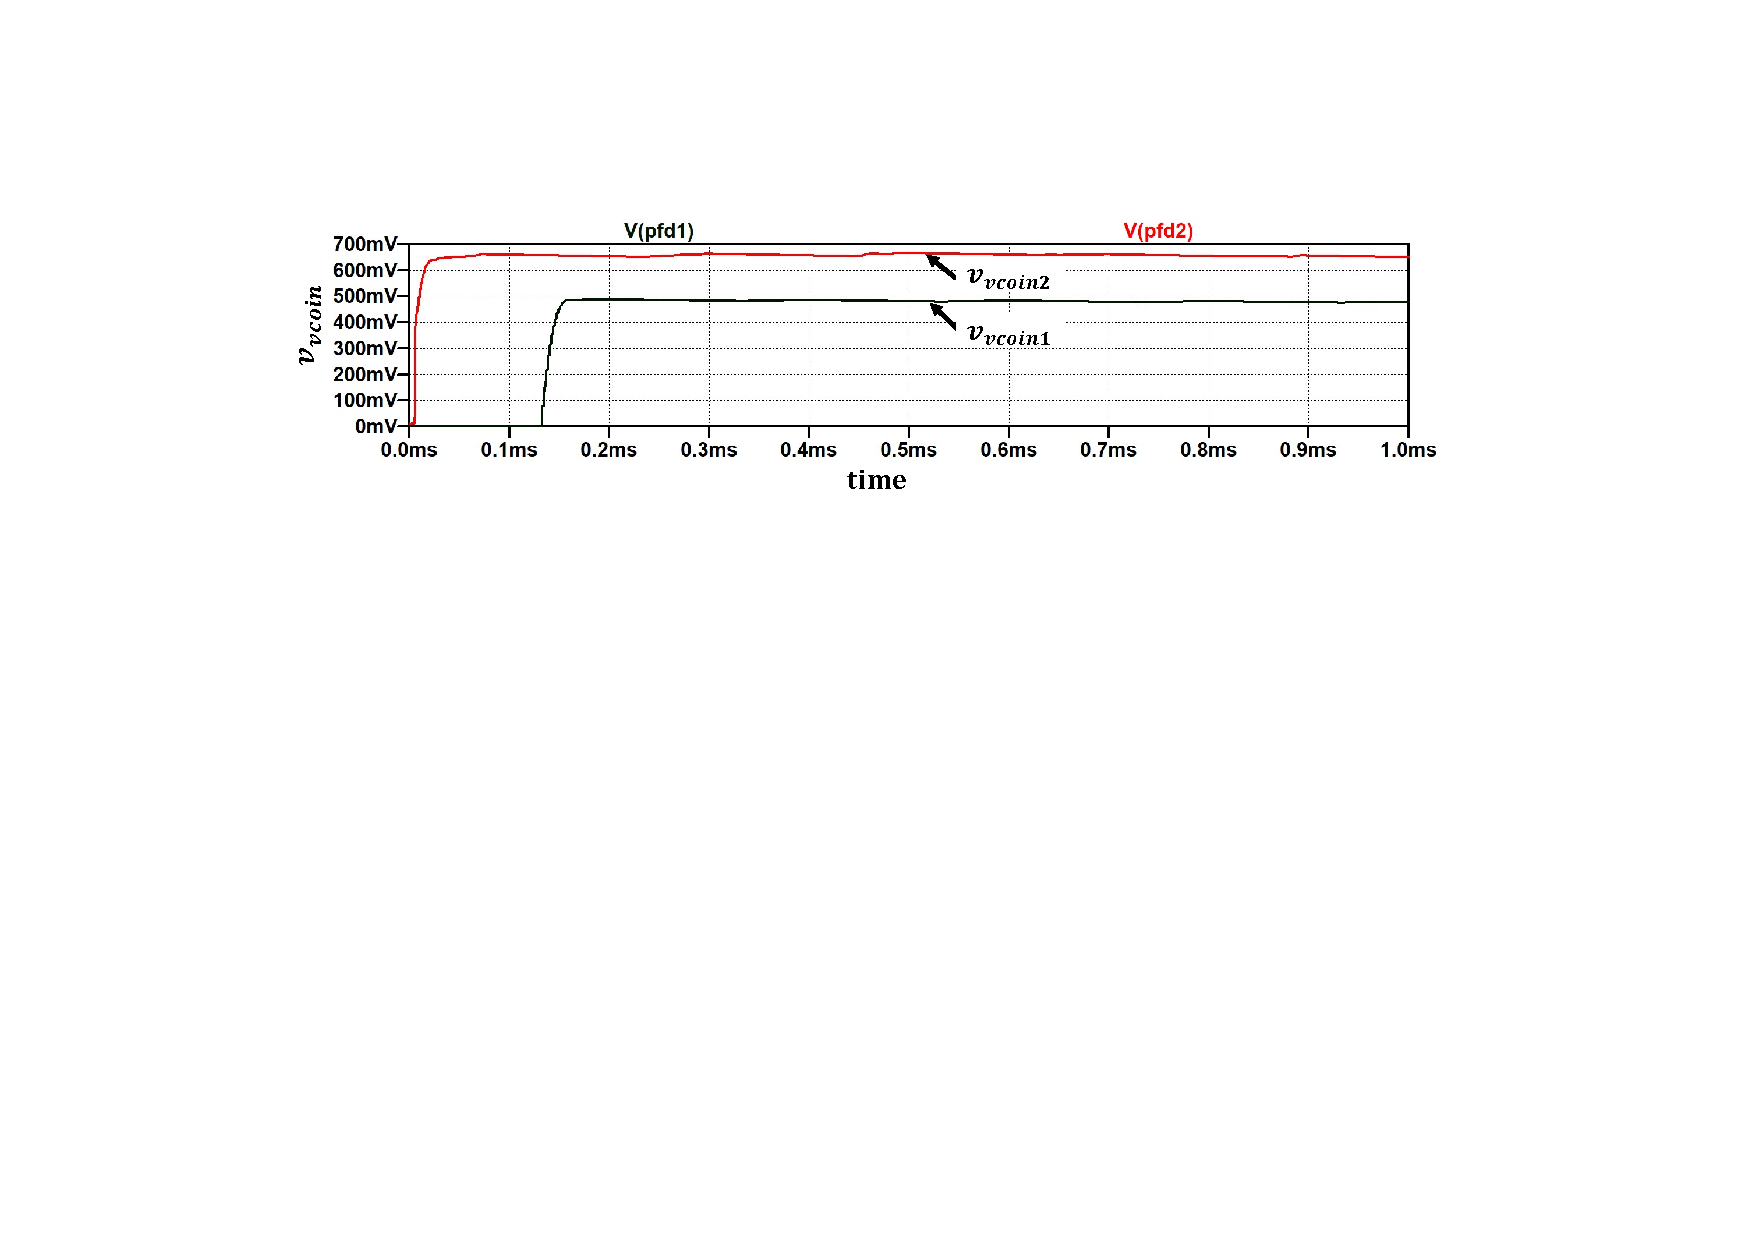
\includegraphics[width=130mm]{figures/fsksimulationgraph1.pdf}
\caption{VCO制御電圧の過渡解析結果}
\label{fsksimulationgraph1}

\vspace{3mm}

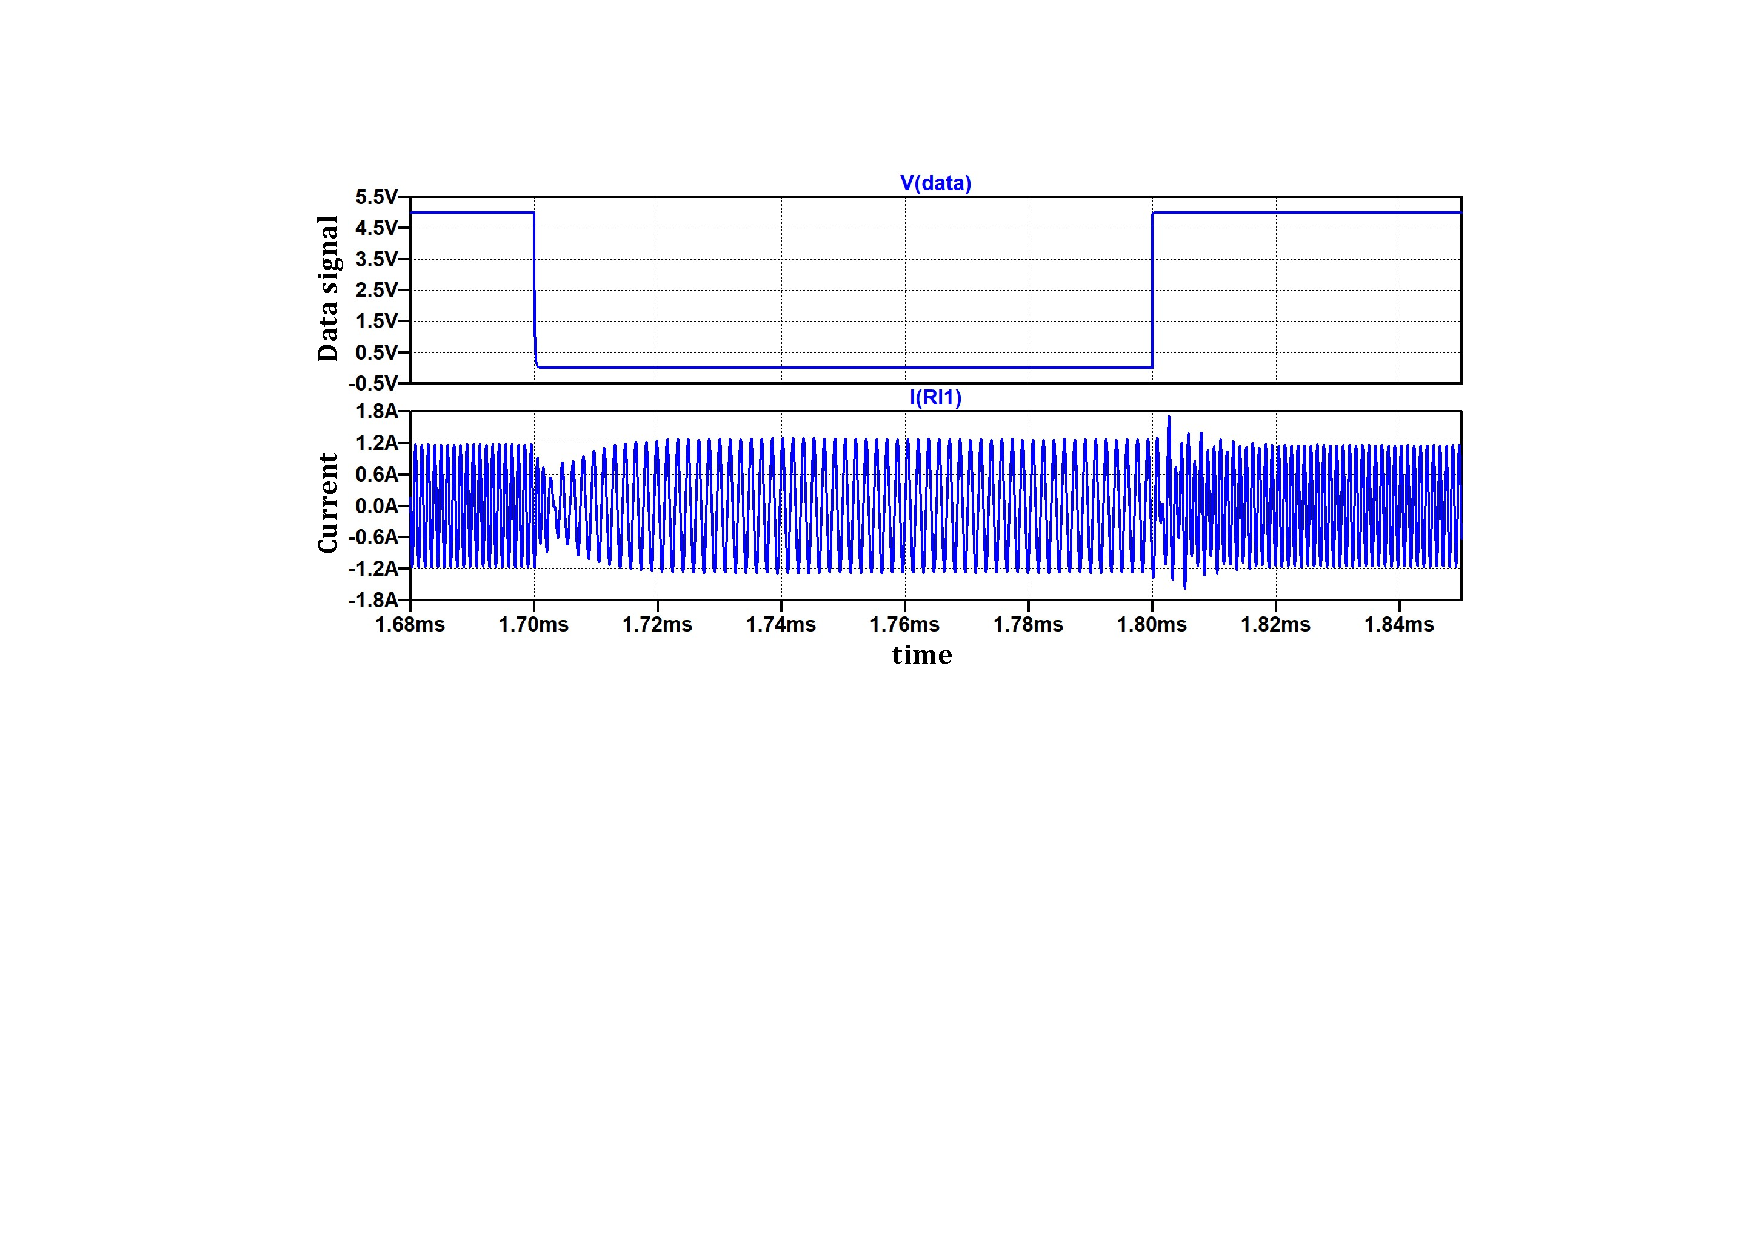
\includegraphics[width=130mm]{figures/fsksimulationgraph2.pdf}
\caption{データ信号(上段)ならびに負荷電流(下段)の過渡解析結果}
\label{fsksimulationgraph2}

\end{center}
\end{figure}

\begin{figure}[!h]
\begin{center}

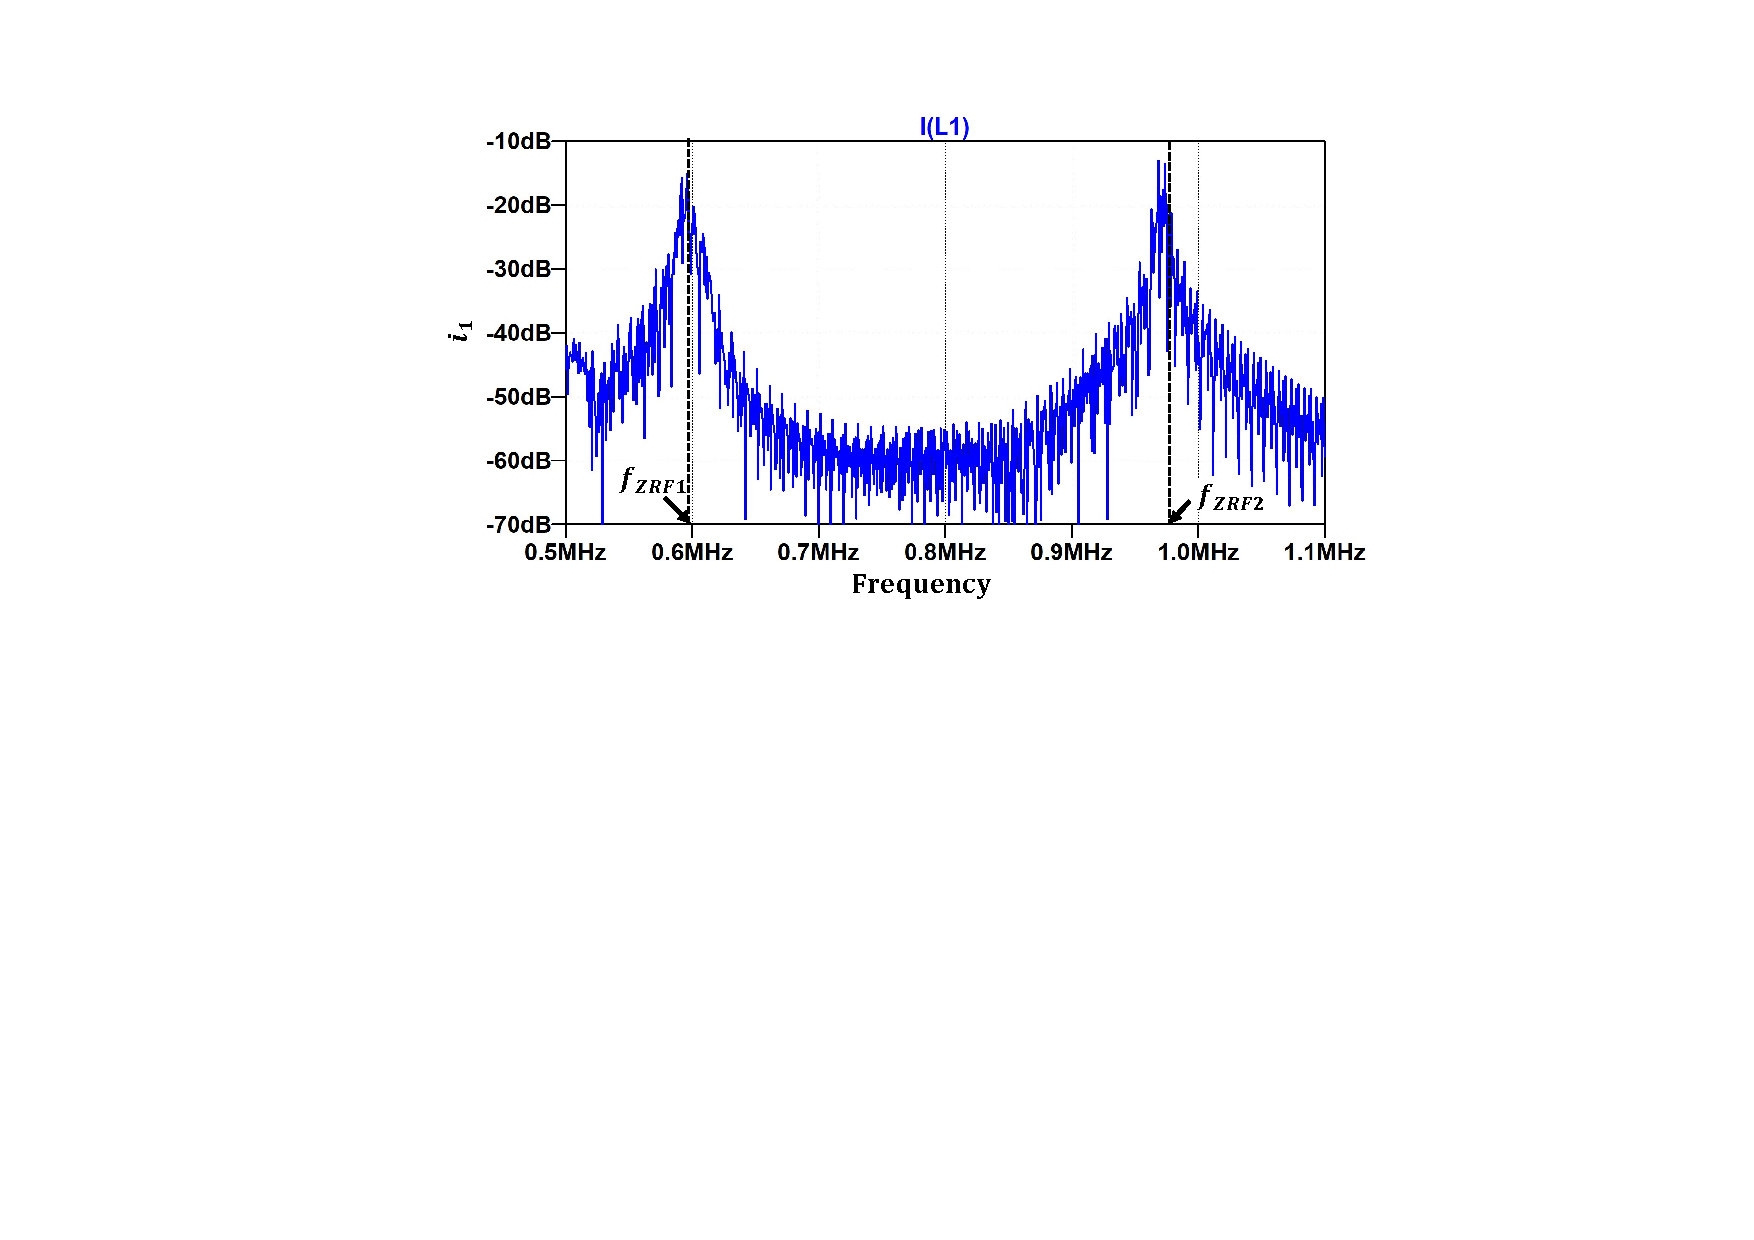
\includegraphics[width=140mm]{figures/fsksimulationgraph3.pdf}
\caption{電流$i_1$のスペクトル}
\label{fsksimulationgraph3}

\end{center}
\end{figure}
\section{FPGAを用いたFSK復調器}
\subsection{FPGAボードの概要}

\begin{figure}[t]
\begin{center}

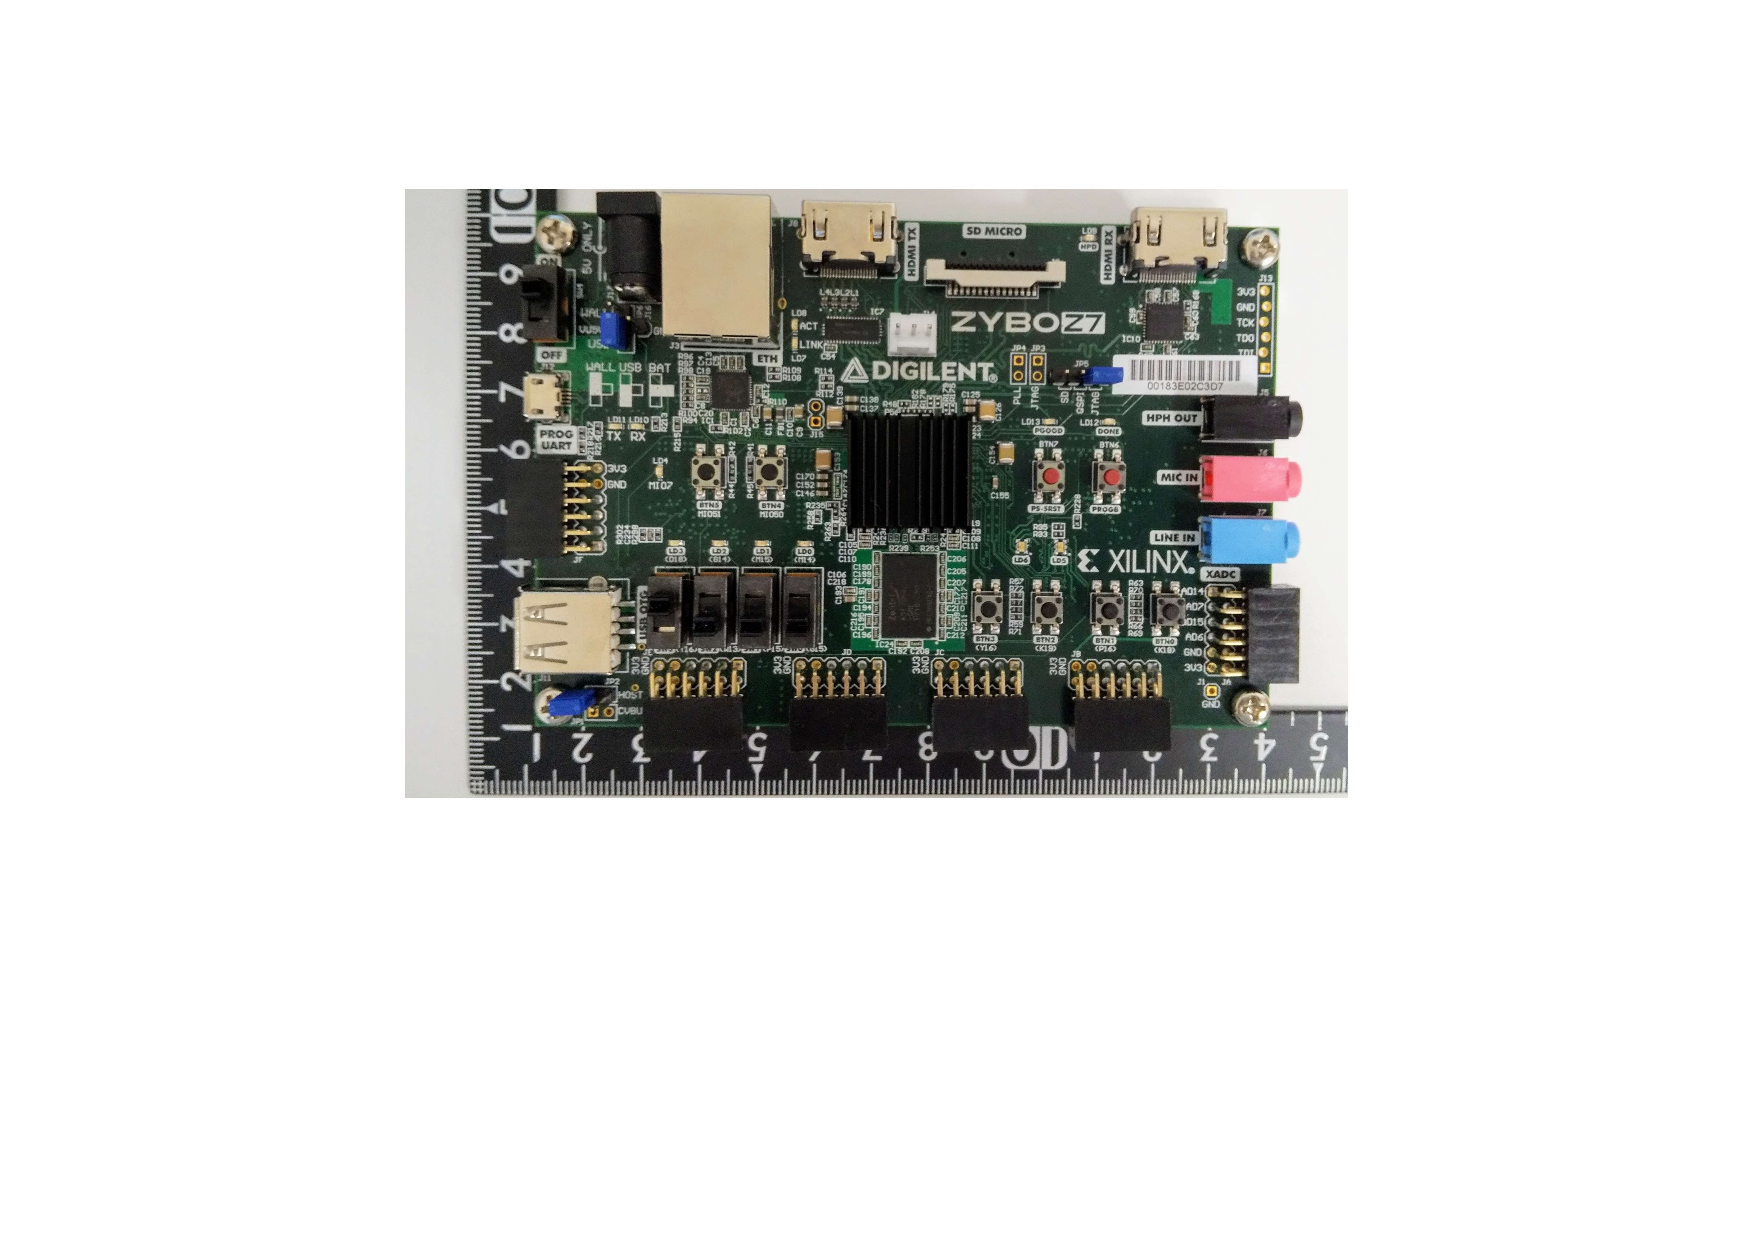
\includegraphics[width=140mm]{figures/fpgaphoto.pdf}
\caption{FPGAボード Zybo Z7-20}
\label{fpgaphoto}

\end{center}
\end{figure}

本研究では,FSK信号の復調用として,図\ref{fpgaphoto}に示すXilinx社のZybo Z7-20(以下Zybo)を使用した.以下,その概要について述べる.\par 
Zyboは,メインFPGAチップであるXilin社のZynq-7020のほか,入出力スイッチ,microSDカードスロット,HDMI端子,オーディオインターフェースなどを備えている.また,ユーザーが任意に書き換えられるロジック(Programmable Logic : PL)のほか,CPU(Processing System : PS)が搭載されている.リアルタイム性が求められる処理はPL部で,他の処理はPS部で行うことにより,高度な処理が実現できる.また,PS部にはLinuxなどのOSを搭載することもでき,Raspberry Piのような使い方をすることも可能である.PL部の記述には,ハードウェア記述言語であるVerilog-HDL\cite{Kobayashi2018,Kimura2009,Kimura2001}またはVHDLを用いる.本研究においてはVerilog-HDLを採用した.なお,PS部の記述は,通常のマイコンと同じようにCやC++などの言語を用いる.また,開発環境はPL部とPS部でそれぞれ別のものが用意されており,PL部は「Vivado」,PS部は「Vitus」というソフトを使う必要がある.\par
ZyboのPS部には$33.3333 \, \mathrm{MHz}$のクロックが供給されている\cite{zybo}.PSの内部にはPLLが搭載されており,この$33.3333 \, \mathrm{MHz}$のクロックを元として,最大4系統,$667\, \mathrm{MHz}$の動作クロックを得ることができる.動作クロックの周波数は,ユーザが任意に指定することができるが,内部PLLの分周器の構成による制限から,指定した周波数と差異が生じることもあり注意が必要である.また,PL部の動作クロックは,PS部のPLLが生成したクロックを用いることができるほか,PL部専用に独立して搭載された$125 \, \mathrm{MHz}$の信号源を利用することができる.本研究では,PS部を使用せずPL部のみで復調器を構成したため,この$125 \, \mathrm{MHz}$のクロックを用いた.\par 

\subsection{FSK復調器の動作原理}
FSK信号の復調方法は,フィルタ法\cite{Araki1985},零交差検波法\cite{Araki1985},PLL検波法\cite{Yanagisawa1998},2次相関器による方法\cite{Gardner1996},2カウンタ法\cite{Sankar2017}など様々なものが提案されている.本研究では,実装ならびに設計変更の容易性,ビットレート,外部インターフェースとの接続を見据えた拡張性などを勘案して,FPGAを用いてカウンタを構成して復調する手法を採用した.以下,その原理について述べる.\par 
FSK信号を復調する最も簡明な方法は,その周波数あるいは周期を測定することであるが,これらを正確かつ高速に行うことは困難である.そこで,本研究においては,FSK信号の半周期におけるFPGAの動作クロックの立ち上がりエッジを計数することにより,間接的に周期を測定する手法を採用した.例として,データが1のときのFSK信号の周波数$f_{mark}=979 \, \mathrm{kHz}$, 0のときのFSK信号の周波数$f_{space}=598 \, \mathrm{kHz}$,FPGAのクロック周波数$f_{clk}=125 \, \mathrm{MHz}$の場合を考える.FSK信号の一周期における$f_{clk}$の立ち上がりエッジを計数するカウンタを構成した場合,FSK信号の周波数が$f_{mark}$のときの計数値$N_{mark}$,$f_{space}$の時の計数値$N_{space}$は,それぞれ
\begin{align}
N_{mark} &=\frac{125 \times 10^6}{979 \times 10^3}\simeq 128 \\
N_{space} &=\frac{125 \times 10^6}{598 \times 10^3} \simeq 209
\end{align}
となる.したがって,FPGA内部にカウンタを構成し,その値が適当なしきい値$N_{th}$より大きいか否かを判定することで,データを復調することができる.\par 
実際のFSK-SWIPTシステムにおいては,$f_{space}, \, f_{mark}$はそれぞれ2つのZRF$f_{ZRF1}, \, f_{ZRF2}$に対応し,2.2節における解析で述べたように$f_{ZRF1}<f_{ZRF0}<f_{ZRF2}$である.したがって,データ判定のしきい値$N_{th}$は$f_{ZRF0}$を基準にして決定すればよい.表1の数値例においては,式(2.12)より$f_{ZRF0} \simeq712 \, \mathrm{kHz}$であるから,
\begin{equation}
N_{th} =\frac{125 \times 10^6}{712 \times 10^3} \times \simeq 176
\end{equation}
となる.

\subsection{FSK単体でのFSK変復調器の動作実験}
前項で述べた手法による復調器が正しく動作するか,FPGA内部にFSK変調器と復調器を併せて実装して確認した.動作確認は,論理シミュレーションならびにFPGA内部にロジックアナライザを構成して波形を測定することにより行った.ロジックアナライザの構成は,Xilinx社の開発ソフトVivadoに標準搭載されている機能であり,外部の測定器を使わずに動作波形を測定することができデバッグに非常に有用である\cite{Kobayashi2018}.また,FSK変復調器ならびにそのテストベンチのVerilog-HDLソースコードを付録Bに添付する.\par
FPGA内部のFSK変調器は,$125 \, \mathrm{MHz}$のクロックを適当に分周して$f_{mark} \simeq 979 \, \mathrm{kHz}$, $f_{space} \simeq 598 \, \mathrm{kHz}$の2つの信号を生成し,それらの信号をデータに対応させて切り替えることによりFSK信号を得る構成とした.データ信号は,クロックを分周して得た,約$57.6 \, \mathrm{kHz}$(115.2kbps相当)の矩形波(101010…の連続信号)とした.\par 
図\ref{logicanalyzer}に,ロジックアナライザにより測定したFSK変復調器の動作波形を示す.同図上段がデータ信号,中段がFSK信号,下段が復調されたデータ信号である.同図より,復調データは元データ信号に対して遅延が生じているものの,正しく復調出来ていることが分かる.図\ref{counter}は,FSK信号の一周期におけるクロックの立ち上がりエッジを計数するカウンタの値の遷移を示したものである.カウンタの値は,データが遷移するときを除き約210回と130回の2値となっており,これは式(4.4),(4.5)の計算結果と一致していることから,カウンタが所望の動作を実現できているといえる.

\begin{figure}[b]
\begin{center}

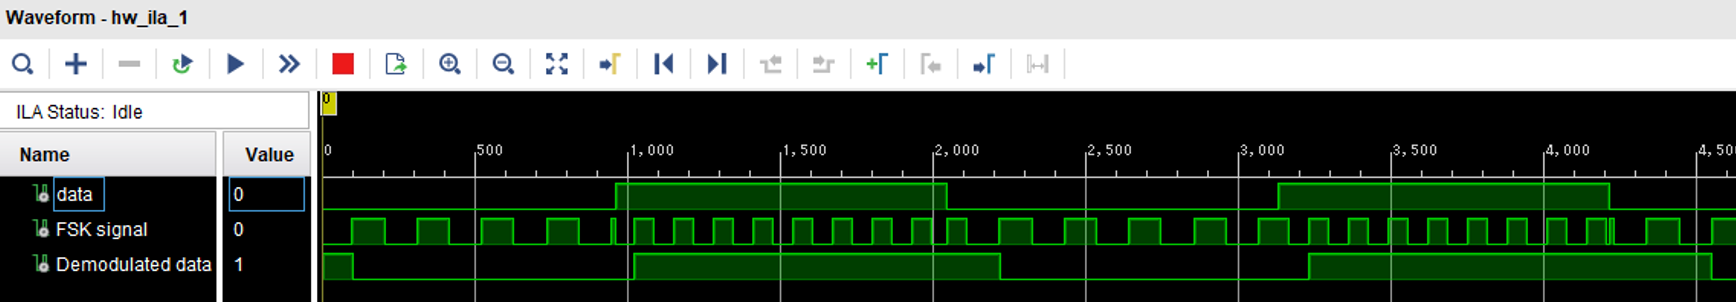
\includegraphics[width=160mm]{figures/logicanalyzer.png}
\caption{FSK変復調器の動作波形}
\label{logicanalyzer}

\end{center}
\end{figure}

\begin{figure}[h]
\begin{center}

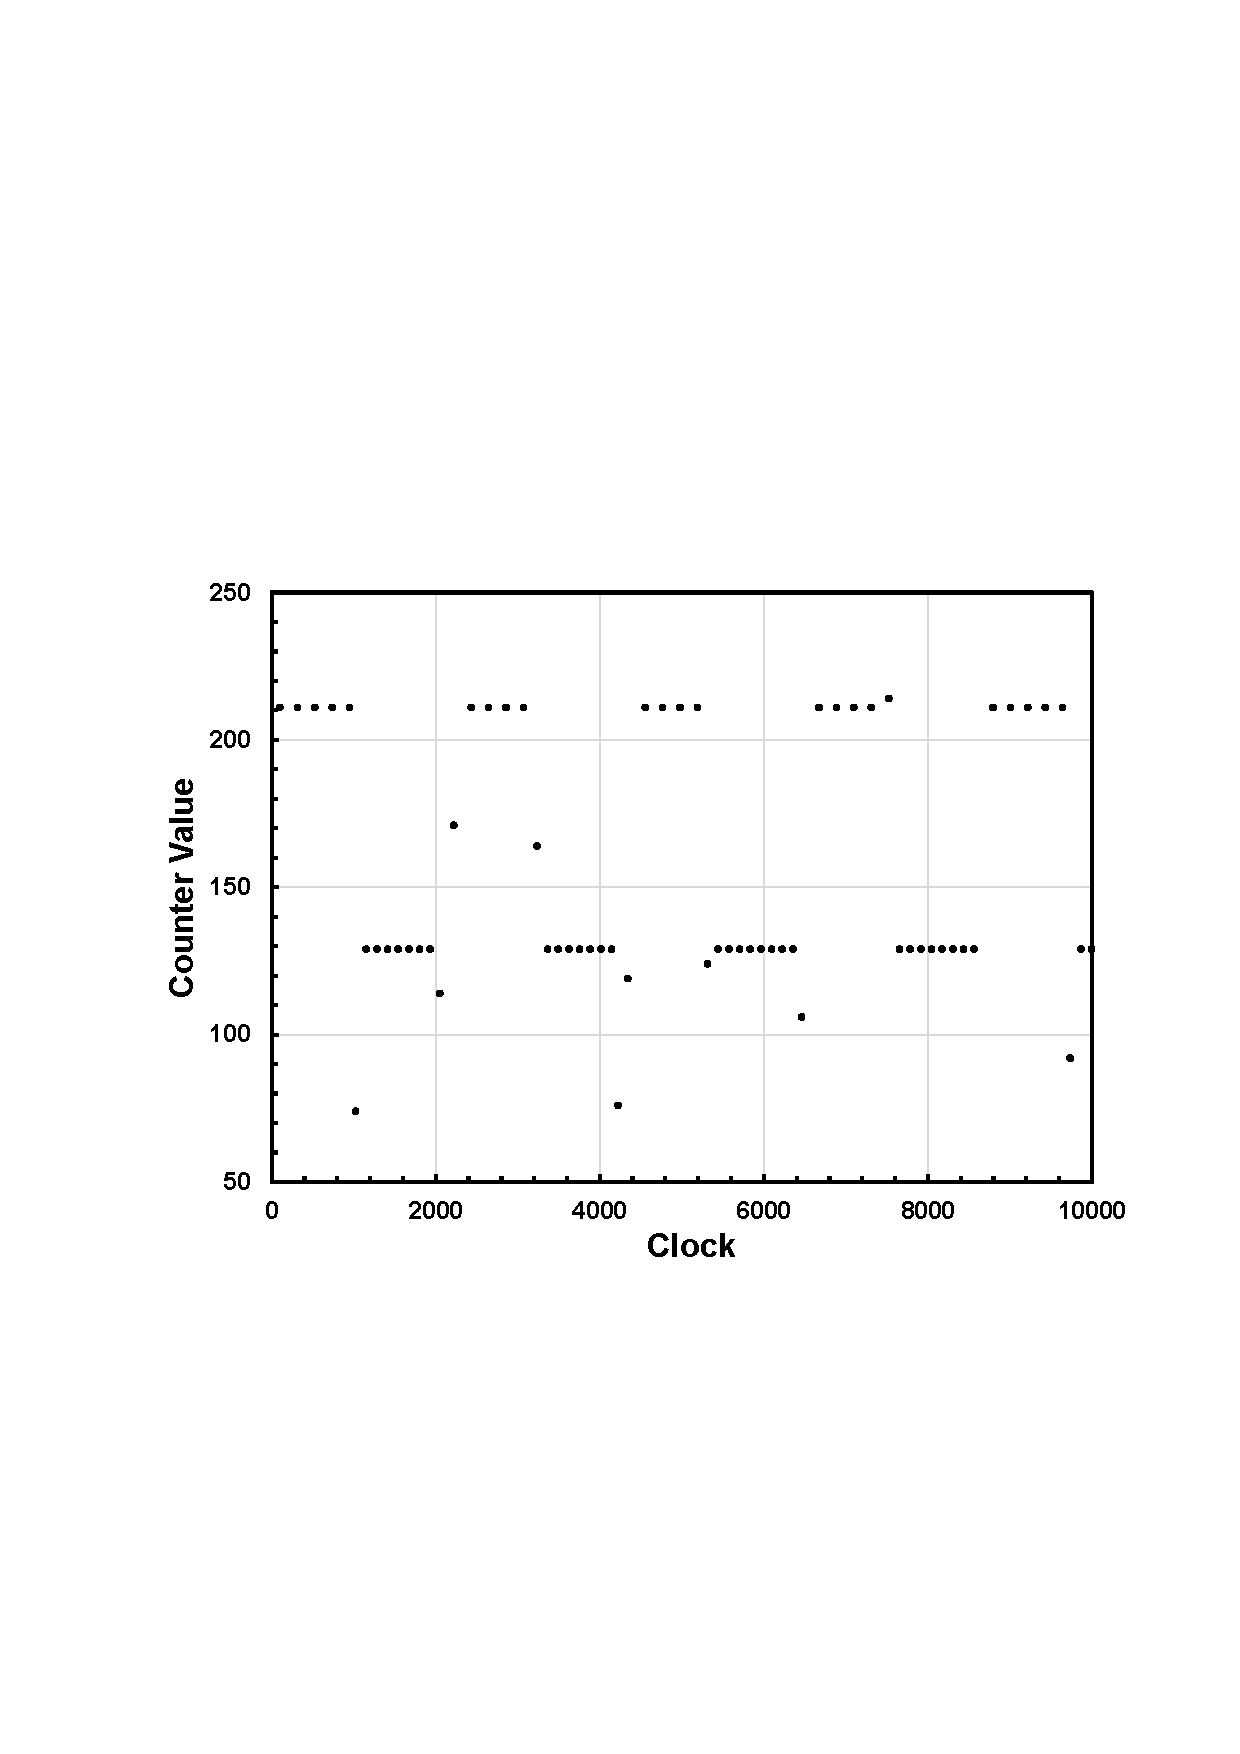
\includegraphics[width=100mm]{figures/counter.pdf}
\caption{カウンタの値の時間遷移}
\label{counter}

\end{center}
\end{figure}

\section{実装ならびに実験}
\subsection{実装回路}
本研究では,提案回路をプリント基板上(Printed Circuit Board : PCB)に実装し,各種特性の測定実験を行った.図\ref{circuitphoto}に,実装した回路の写真を示す.また,設計した回路の全体回路図ならびにPCBのレイアウト図を付録Aに添付する.実装回路の主要なICの型番ならびに回路定数を表4.1に示す.

\begin{table}[h]
\centering
\caption{主要なICならびに回路定数 (定数は100 kHzにて測定)}
\begin{tabular}{c|c|c}
\hline
\multicolumn{1}{c|}{素子} & \multicolumn{1}{c|}{型番/定数} & \multicolumn{1}{c}{メーカー} \\ \hline
PLL & CD74HC4046 & Texas Instruments \\ \hline
ハーフブリッジドライバ & ADuM3223 & Analog Devices\\ \hline
ハーフブリッジ用NchMOSFET & RD3L220SN & Rohm \\ \hline
送電コイル$L_1$ & $3.86\, \mathrm{\mu H}$, \, ESR : $0.053\, \mathrm{\Omega}$ & - \\ \hline
受電コイル$L_2$ & $3.91\, \mathrm{\mu H}$, \, ESR : $0.034\, \mathrm{\Omega}$ & - \\ \hline
送電側共振キャパシタ$C_1$ & $10.05\, \mathrm{n F}$, \, ESR : $0.043\, \mathrm{\Omega}$ & - \\ \hline
受電側共振キャパシタ$C_2$ & $10.07\, \mathrm{n F}$, \, ESR : $0.052\, \mathrm{\Omega}$ & - \\ \hline
\end{tabular}
\end{table}

\begin{figure}[p]

	\begin{center}
    \subfloat[送電側]{
    \includegraphics[width=150mm]{figures/transmitterphoto.png}
    }
    \\ \vspace{5mm}
    \subfloat[受電側]{
    \includegraphics[width=130mm]{figures/receiverphoto.png}
    }
	\end{center}
    
  \caption{実装回路}\label{circuitphoto}
\end{figure}

\subsection{実験}
実装回路の特性を調査するため,以下の7種の実験を行った.本項では,それらの実験の方法ならびに結果について順に述べる.実験に使用した測定器を表4.2に示す.

\begin{itemize} \setlength{\itemsep}{-0.2cm}
\item コイル間距離-結合係数特性の測定
\item ZRFの手動追従実験
\item ZRFの自動追従実験
\item データ伝送時の出力スペクトルの測定
\item データ伝送速度-電力効率特性の測定
\item 文字列データ伝送実験
\item 符号誤り率(Bit Error Rate : BER)の測定
\end{itemize}

\begin{table}[h]
\centering
\caption{測定機器}
\begin{tabular}{c|c|c}
\hline
\multicolumn{1}{c|}{名称} & \multicolumn{1}{c|}{型番} & \multicolumn{1}{c}{メーカー} \\ \hline
高周波電圧計(True RMS) & 3400A & Hewlett-Packard \\ \hline
周波数カウンタ & 5535A & Hewlett-Packard \\ \hline
スペクトラムアナライザ & 8561A & Hewlett-Packard \\ \hline
直流電源装置 & KPS3010D & Wanptek\\ \hline
信号発生器 & MHS-5200A & KKmoon \\ \hline
BER測定器 & ME448B & Anritsu \\ \hline
\end{tabular}
\end{table}

\subsubsection{コイル間距離-結合係数特性の測定}
はじめに予備実験として,送受電コイル間の距離$d$と結合係数$k$の測定を行った.このときの測定系を図\ref{dvsk}に示す.同図において,$L_1, L_2$はそれぞれ送受電コイル,$r_{L1},r_{L2}$はそれらのESRである.また,本実験を含め,本稿で報告する実験で用いた高周波電圧計はすべて真の実効値を指示するものである.本実験の測定手順を以下に示す.

\begin{enumerate}
  \item 信号発生器から周波数$1 \, \mathrm{MHz}$の正弦波を出力し,高周波電圧計の指示値$v_1$が$1 \, \mathrm{V}$となるよう信号発生器の出力振幅を調整した.
  \item 信号発生器の出力を保ちながら,高周波電圧計を受電側に付け替え,コイル間の距離$d$を$5 \, \mathrm{mm}$から$13 \, \mathrm{mm}$まで$1 \, \mathrm{mm}$ずつ変化させたときの受電コイルの電圧$v_{out}$を測定した.送受電コイルは,距離の測定を容易にするため,図\ref{coilphoto}のように方眼紙上で相対させた.
  \item 同様の測定を3回行い,各距離における受電コイルの電圧$v_{out}$の平均$v_{outave}$を求めた.
  \item 次の近似式
  \begin{align}
	k \simeq \sqrt{\frac{L_1}{L_2}} \cdot \frac{v_{outave}}{v_1} =\sqrt{\frac{L_1}{L_2}} \cdot v_{outave}
  \end{align}
を用いて,各距離における結合係数$k$を求めた.
\end{enumerate}
距離$d$と結合係数$k$の測定結果を図\ref{dvskgraph}に示す.なお,今回は$k$がある程度大きい領域($k>0.3$程度)での実験を企図していたため,測定は$d=13 \, \mathrm{mm}$で打ち切った.

\begin{figure}[h]
\begin{center}
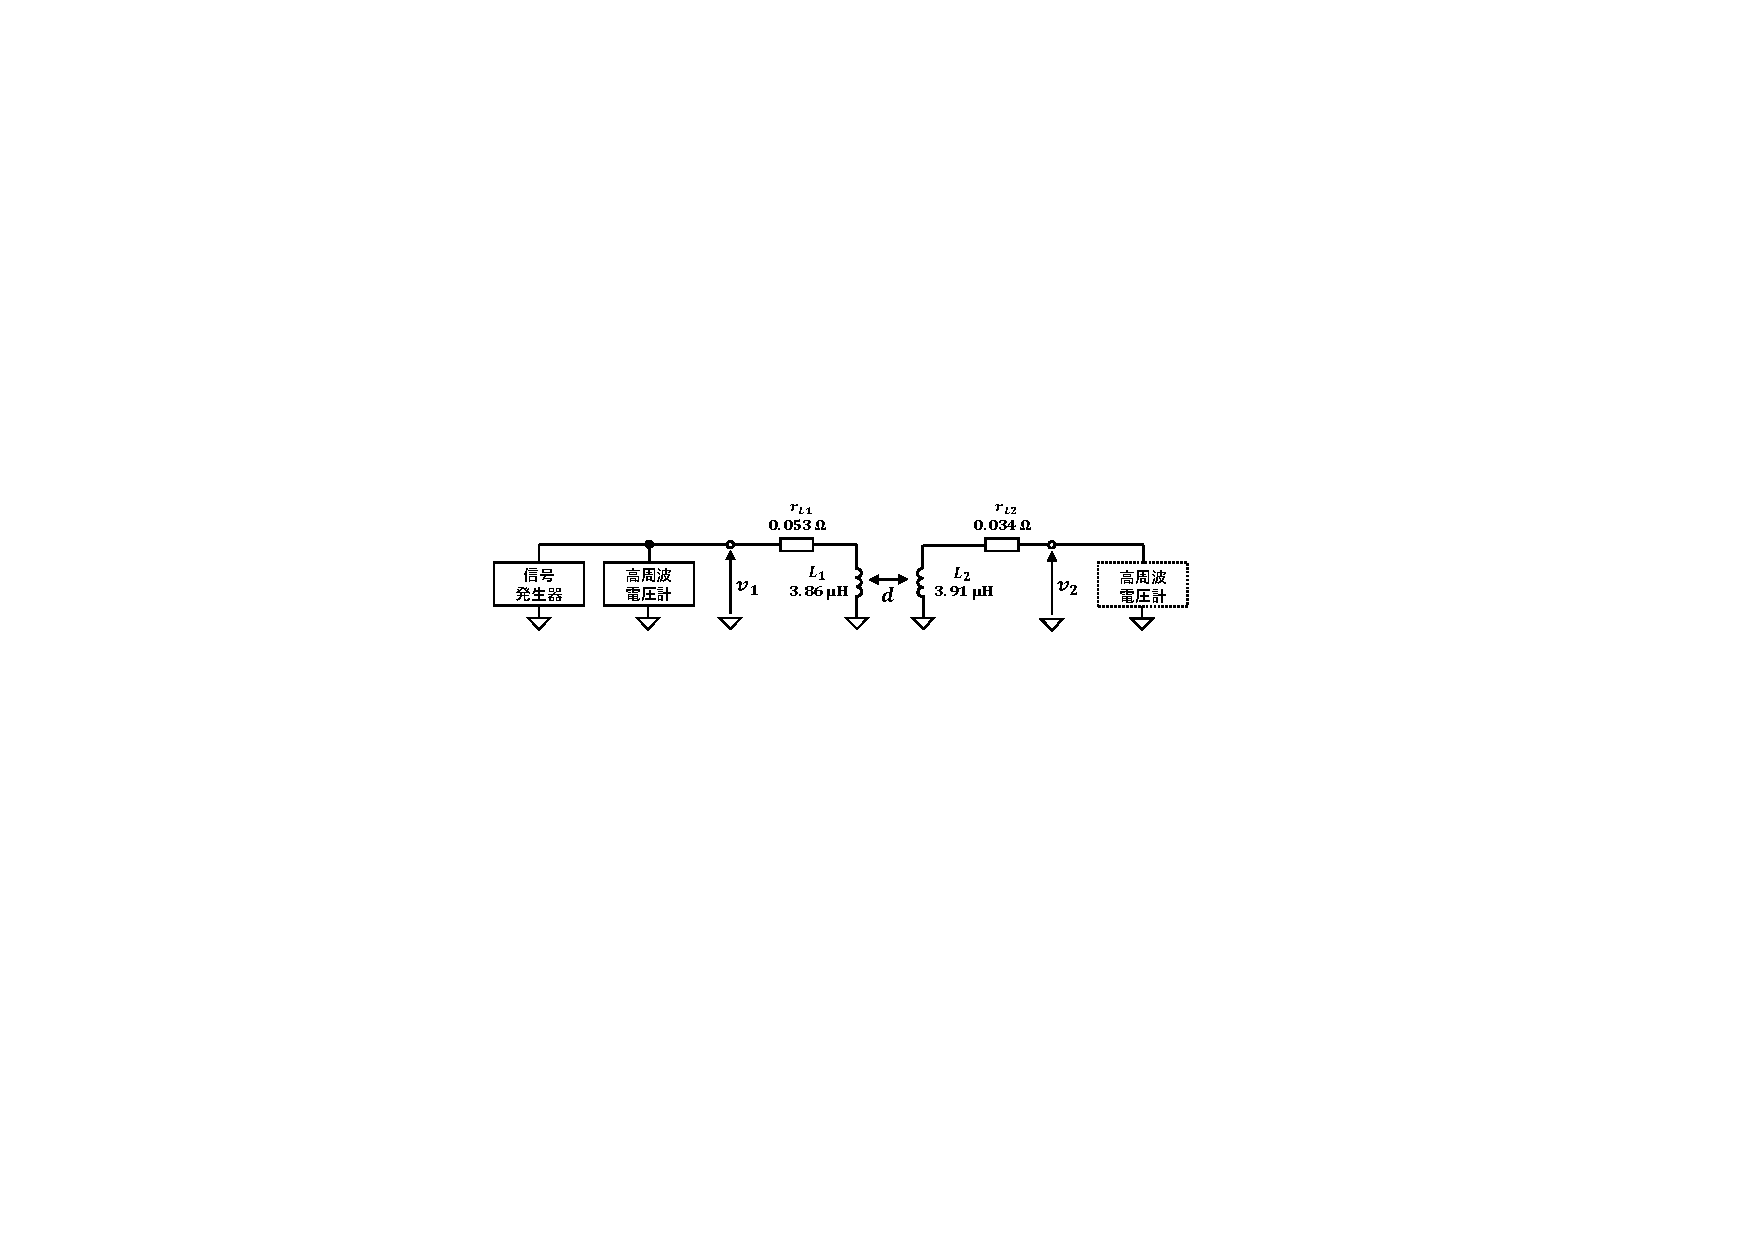
\includegraphics[width=160mm]{figures/dvsk.pdf}
\caption{コイル間距離-結合係数特性の測定系}
\label{dvsk}
\end{center}
\end{figure}

\begin{figure}[h]
  \centering
    \begin{tabular}{c}
       \begin{minipage}{0.50\hsize}
        \centering
          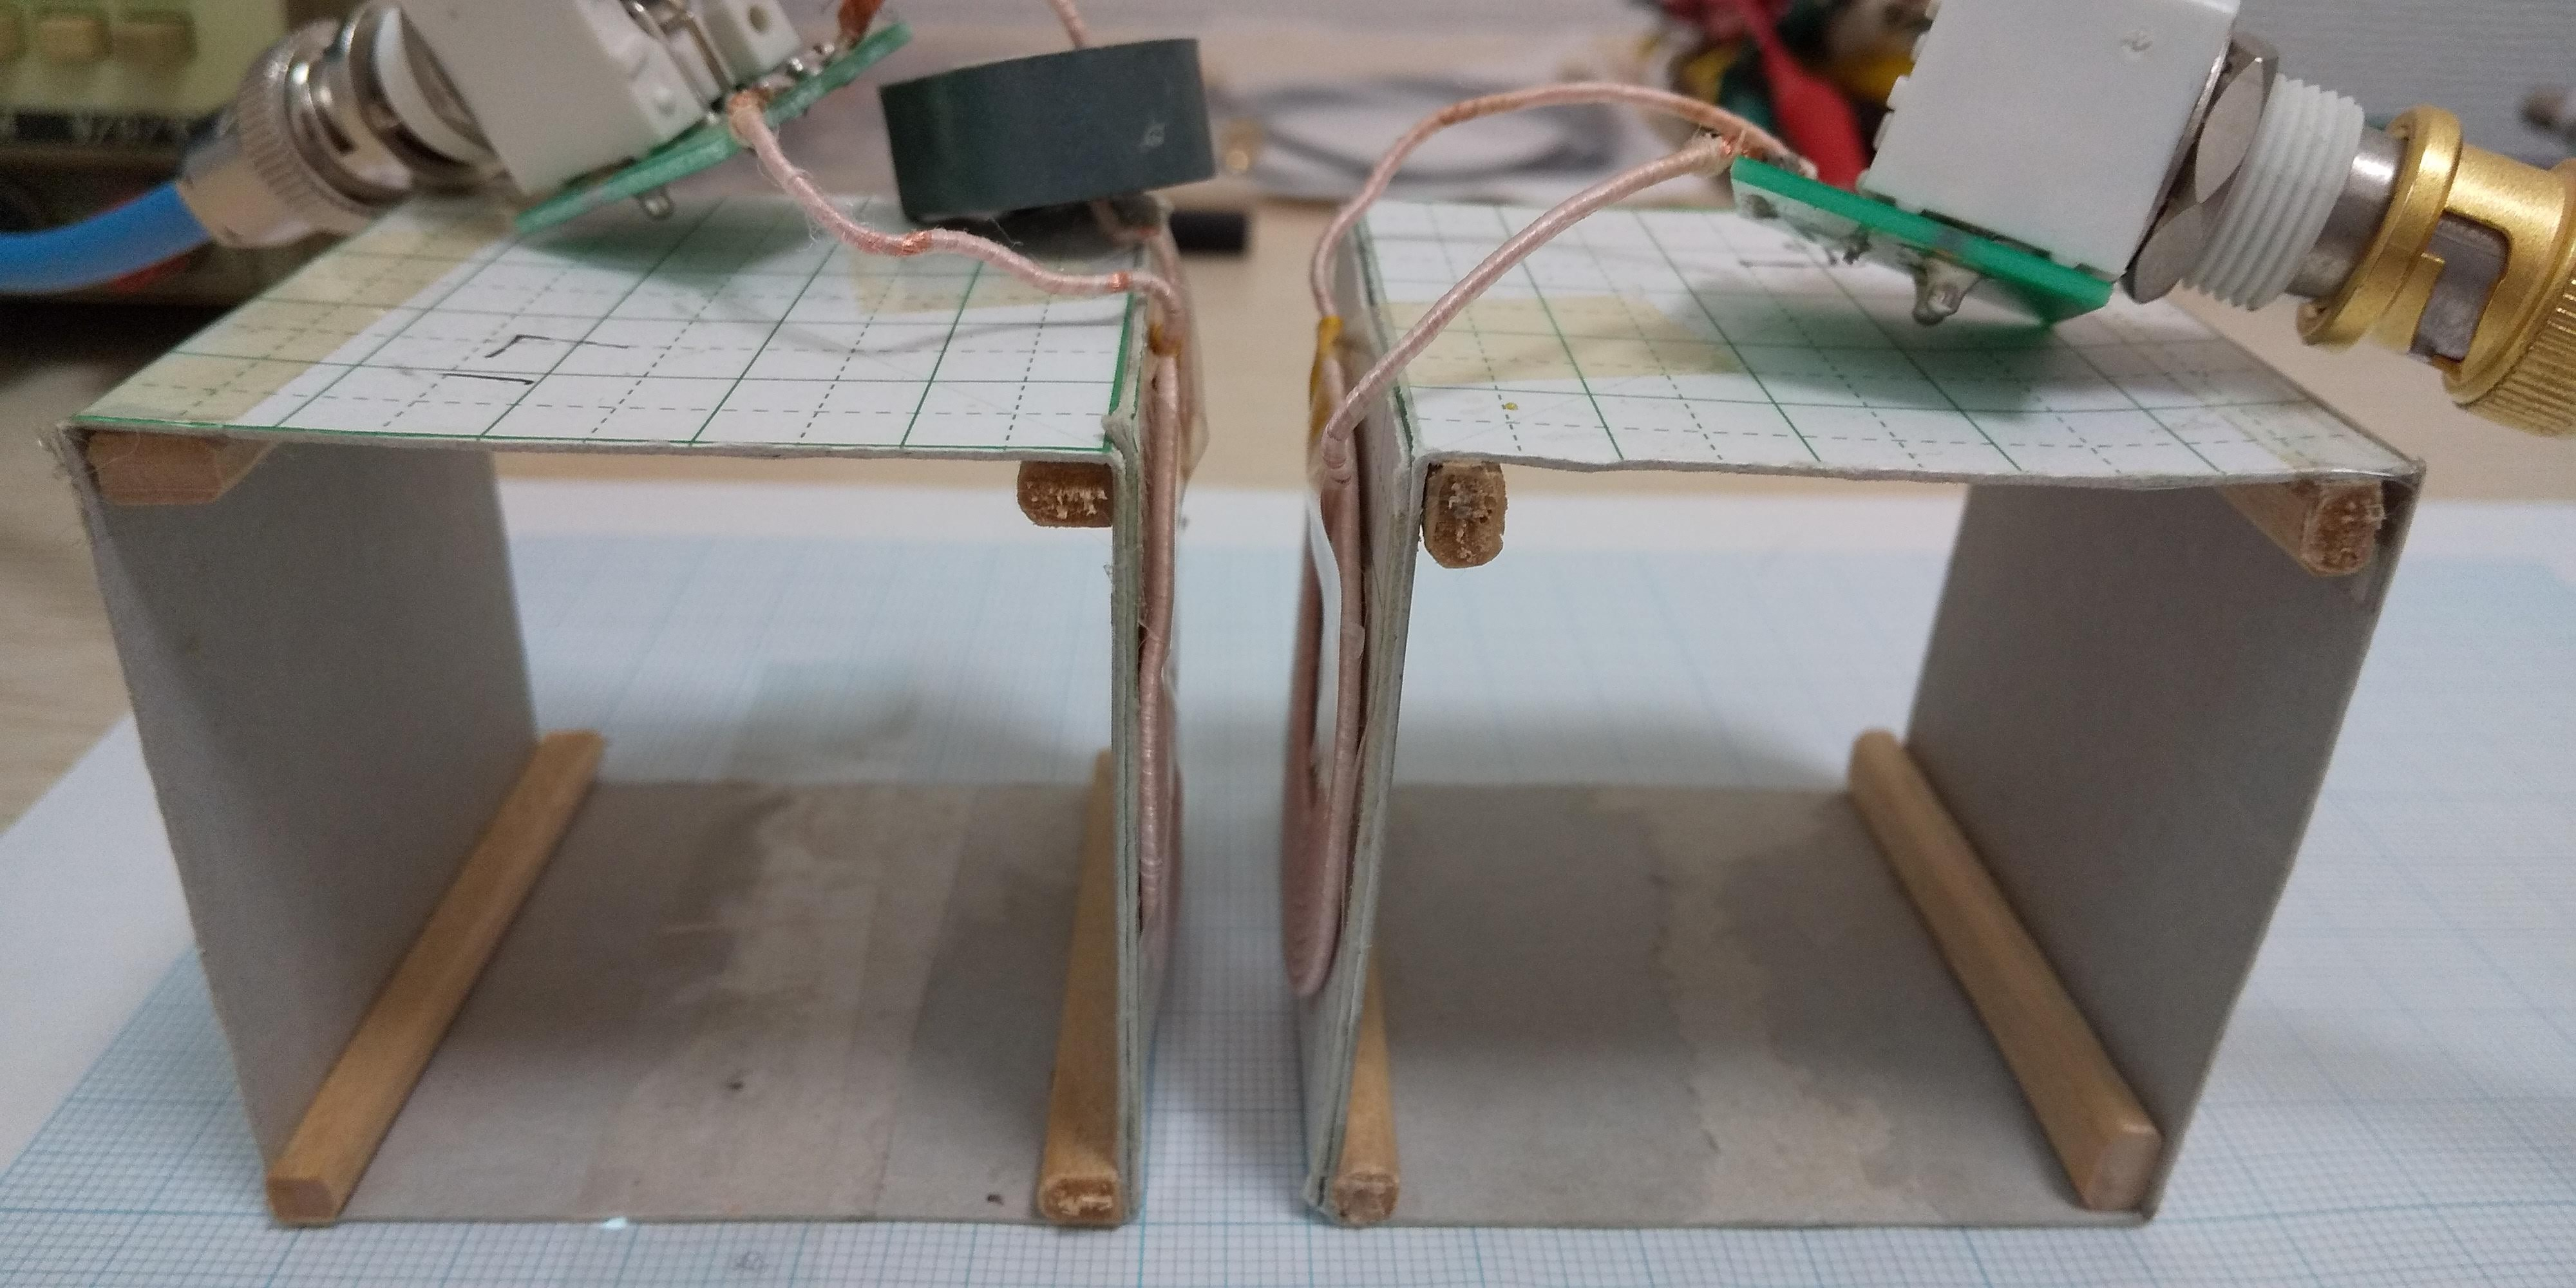
\includegraphics[width=75mm]{figures/coilphoto.jpg}
                          \caption{結合係数特性の測定風景}
                          \label{coilphoto}
      \end{minipage}
  \hspace{5mm}
      \begin{minipage}{0.50\hsize}
        \centering
          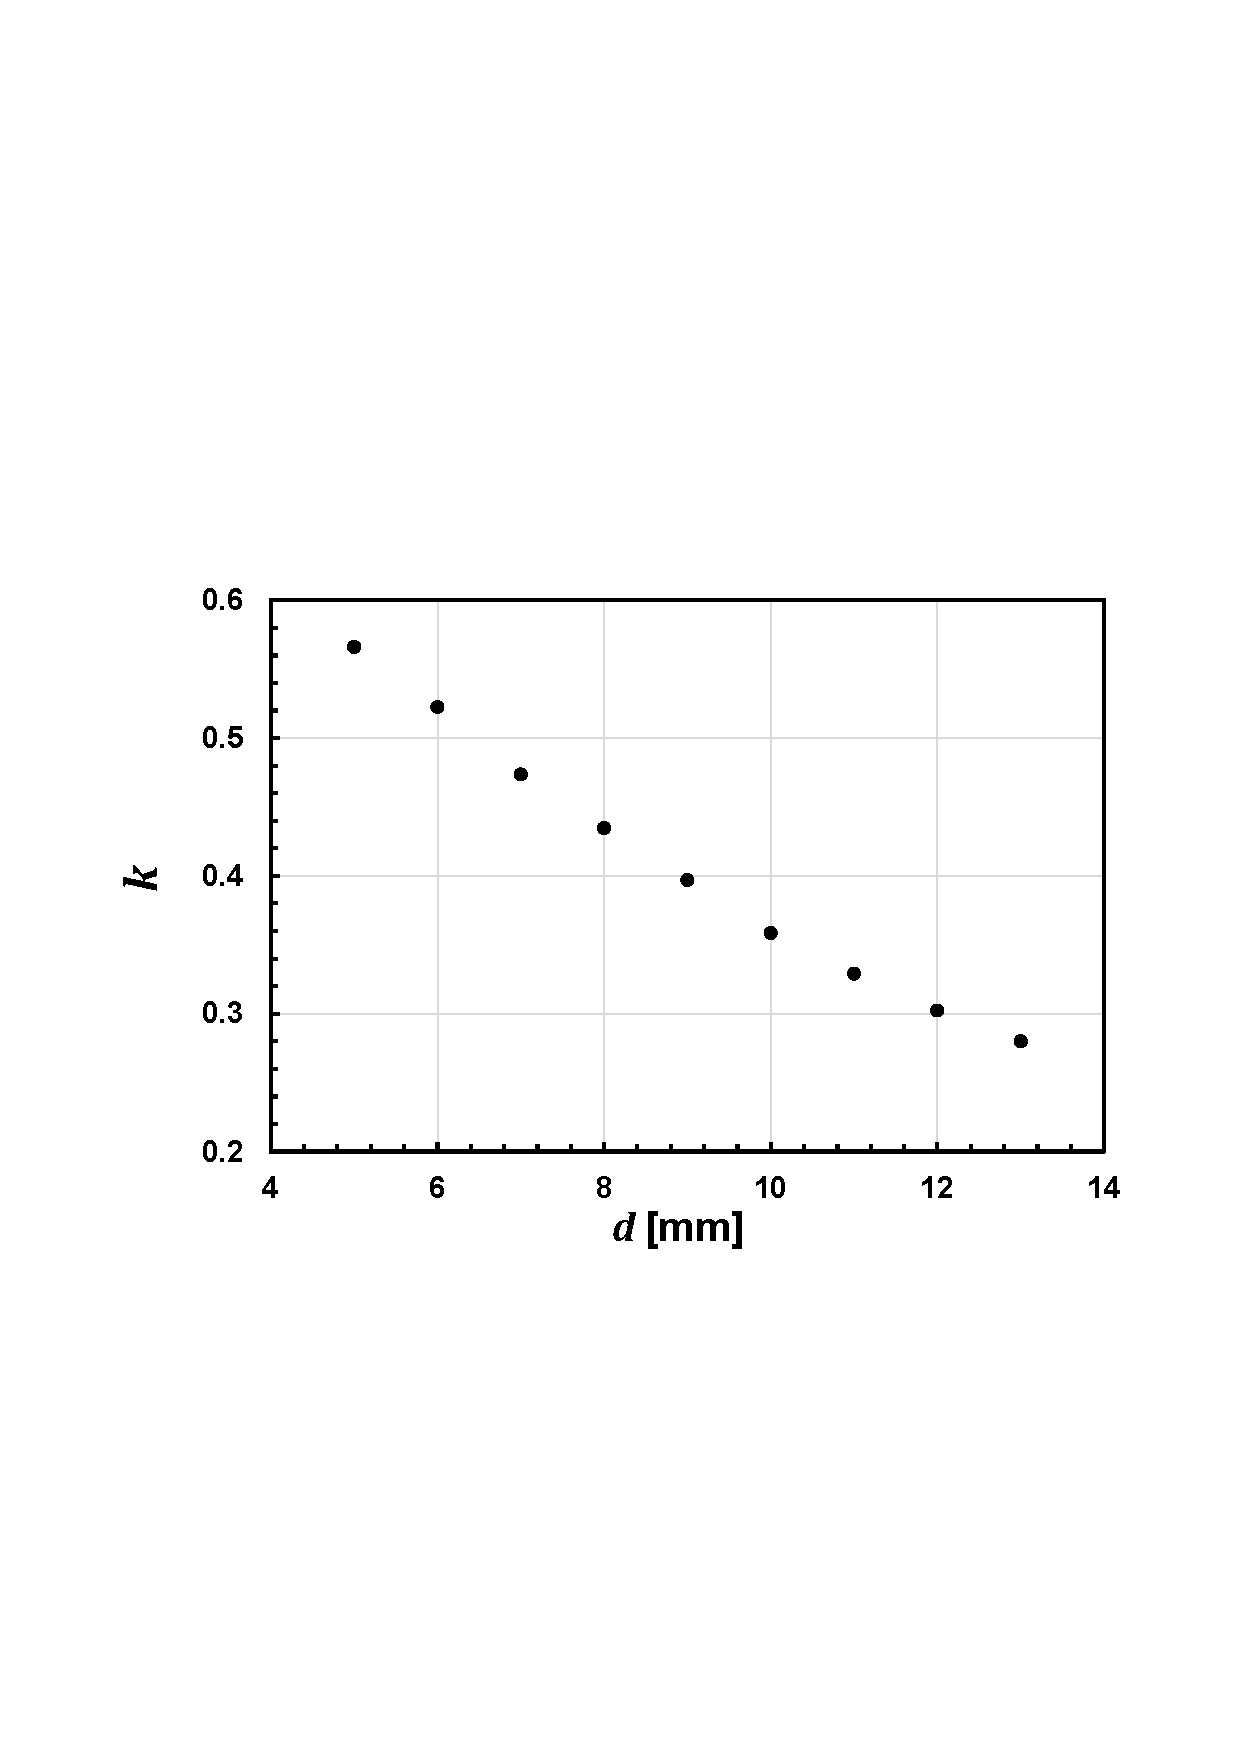
\includegraphics[width=75mm]{figures/dvskgraph.pdf}
                          \caption{コイル間距離-結合係数特性の測定結果}
						  \label{dvskgraph}
      \end{minipage} \\
     \end{tabular}
\end{figure}  


\subsubsection{ZRFの手動追従}
PLLによる自動追従動作を確認する前に,先ずはZRFを手動で追従することにより,各コイル間距離$d$における2つのZRF$f_{ZRF1},f_{ZRF2} \, (f_{ZRF1}<f_{ZRF2})$と,各ZRFにおける電力効率を測定した.このときの測定系を図\ref{manual}に示す.同図において,$C_1, C_2$はそれぞれ送受電側の共振キャパシタ,$r_{1},r_{2}$はそれぞれ$L_1$と$C_1$,$L_2$と$C_2$の合成ESRであり,値はLCRメータを用いて周波数$100 \, \mathrm{kHz}$で測定したものである.また,$R_L$は負荷抵抗である.本実験の測定手順を以下に示す.

\begin{enumerate}
  \item コイル間距離$d =5 \, \mathrm{mm}$, ハーフブリッジの入力電圧$V_{in}=5 \, \mathrm{V}$とした.
  \item 位相比較器の出力$V_{PD}$が極小となる(i.e. スイッチング電圧とスイッチング電流の位相差が最小になる)ように信号発生器の出力周波数$f$を調整した.$V_{PD}$が極小となる周波数のうち,最低のものを$f_{ZRF1}$,最高のものを$f_{ZRF2}$として記録した.
  \item 各ZRFにおける直流電源装置の出力電流$I_{in}$ならびに受電側の負荷電圧$v_{out}$を記録し,電力効率$\eta$を
  \begin{align}
  \eta=\frac{v_{out}^2/R_L}{V_{in}I_{in}}
  \end{align}
  として求めた.
  \item コイル間距離を$1 \, \mathrm{mm}$ずつ$13 \, \mathrm {mm}$まで変化させ,同様の測定を行った.
\end{enumerate}
なお,本実験の結果については次項でまとめて述べる.

\subsubsection{PLLによるZRFの自動追従}
次に,マルチプレクサの出力をドライバ回路に接続し,ZRFをPLLにより自動追従させる実験を行った.このときの測定系を図\ref{auto}に示す.実験手順は次のとおりである.

\begin{enumerate}
  \item コイル間距離$d =5 \, \mathrm{mm}$, ハーフブリッジの入力電圧$V_{in}=5 \, \mathrm{V}$とした.
  \item データ入力をHIGH(電源電圧レベル)とした.このとき,マルチプレクサによりPLL1の出力が選択され,回路が正しく動作すればドライバ回路の出力周波数$f_{sw}$は$f_{ZRF2}$でロックされる.
  \item ドライバ回路の出力周波数$f_{sw}$を周波数カウンタで測定し,$f_{ZRF2}$として記録した.また,直流電源装置の出力電流$I_{in}$ならびに受電側の負荷電圧$v_{out}$を記録し,電力効率$\eta$を求めた.
  \item コイル間距離を$1 \, \mathrm{mm}$ずつ$13 \, \mathrm {mm}$まで変化させ,同様の測定を行った.
  \item データ入力をLOW(GNDレベル)として,$f_{sw}$が$f_{ZRF1}$でロックされるようにした上で,以上の測定を繰り返した.
  \item ここまでの測定を計3回行い,その平均値を結果とした.
\end{enumerate}
図\ref{tracking1}に,手動/自動追従によるZRFの測定結果ならびに理論曲線を示す.同図中において,実線が理論曲線,▲印が手動追従,●印が自動追従の測定結果である.なお,測定はコイル間距離$d$をパラメータとして行ったが,図では前々項における実験の結果を用いて$k$をパラメータとしている.同図より,手動/自動追従におけるスイッチング周波数$f$はほぼ等しく,自動追従回路が正しく動作しているものと考えられる.\par
図\ref{tracking2}は,手動/自動追従させた場合の各ZRFにおける電力効率の測定結果である.各ZRFにおける電力効率は,手動の場合と自動の場合とで概ね等しいことがわかる.また,結合係数$k$に対してほぼフラットな特性が得られている.2つのZRFにおける電力効率の差(i.e. 出力電力の差)はおおむね3\%程度であり,これは一次側共振回路と二次側共振回路の共振周波数が等しい($L_1C_1=L_2C_2$)のときに,2つのZRFにおける出力電力が等しくなるという解析結果と対応するものと考えられる(現実的には$L_1C_1=L_2C_2$とならないため,3\%程度の差が生じたと推察される).

\vspace{1cm}

\begin{figure}[h]
\begin{center}
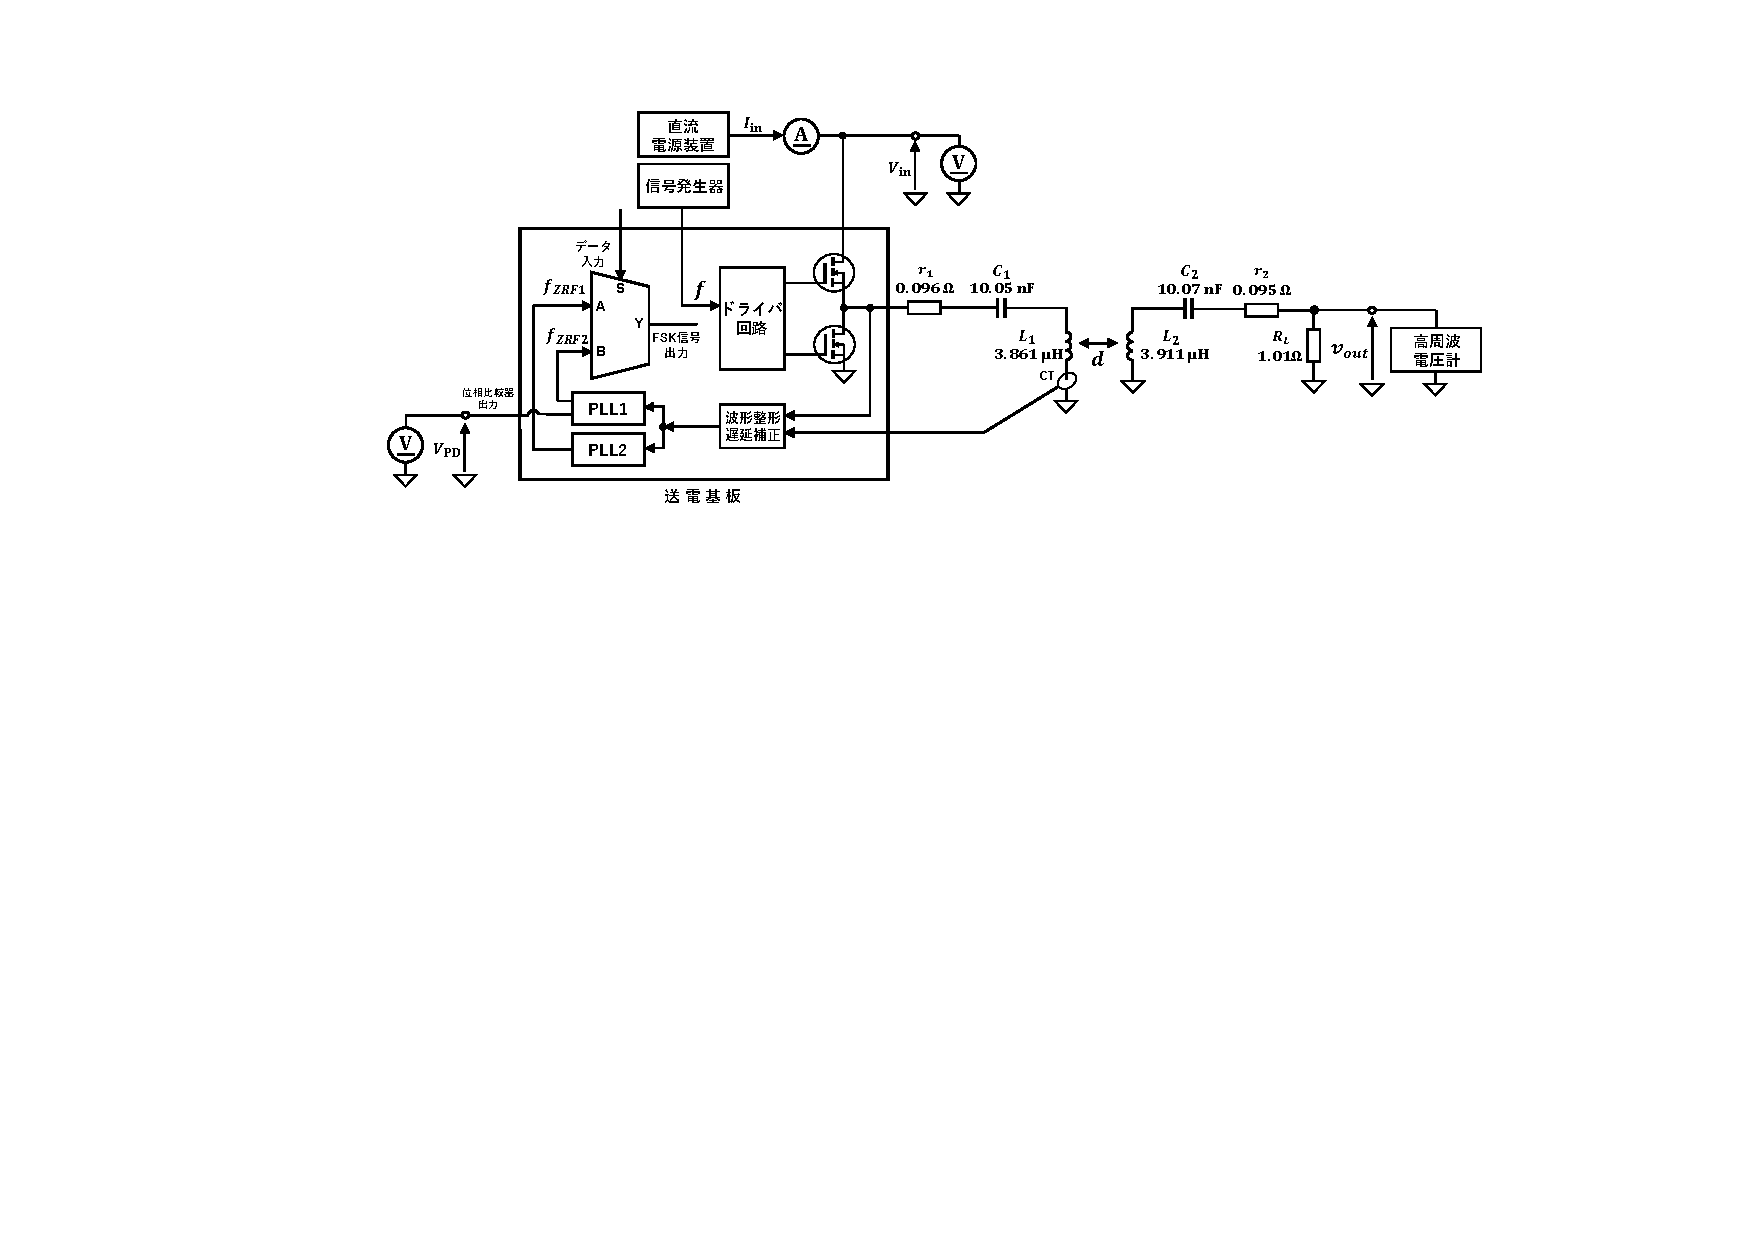
\includegraphics[width=160mm]{figures/manual.pdf}
\caption{ZRFの手動追従実験の測定系}
\label{manual}
\vspace{1cm}

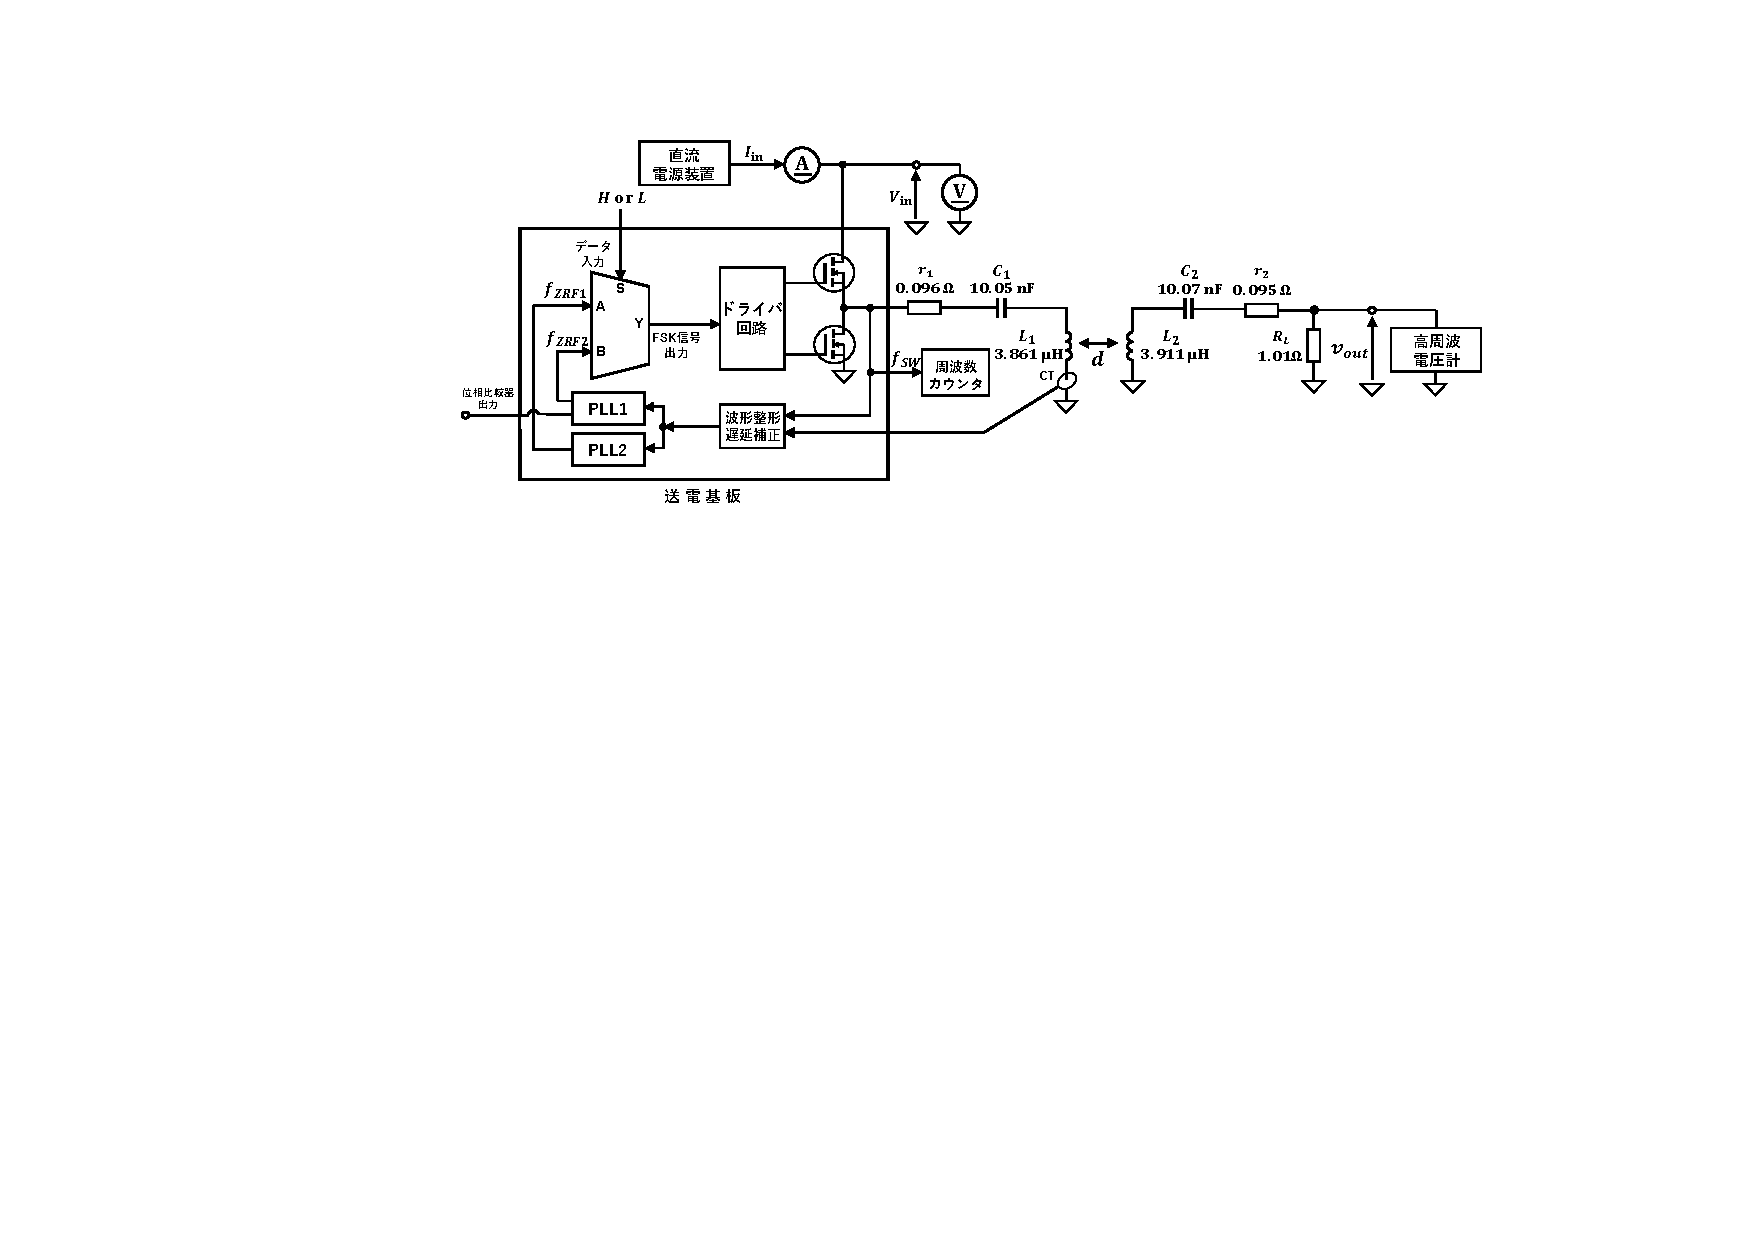
\includegraphics[width=160mm]{figures/auto.pdf}
\caption{ZRFの自動追従実験の測定系}
\label{auto}

\end{center}
\end{figure}

\begin{figure}[p]
\begin{center}
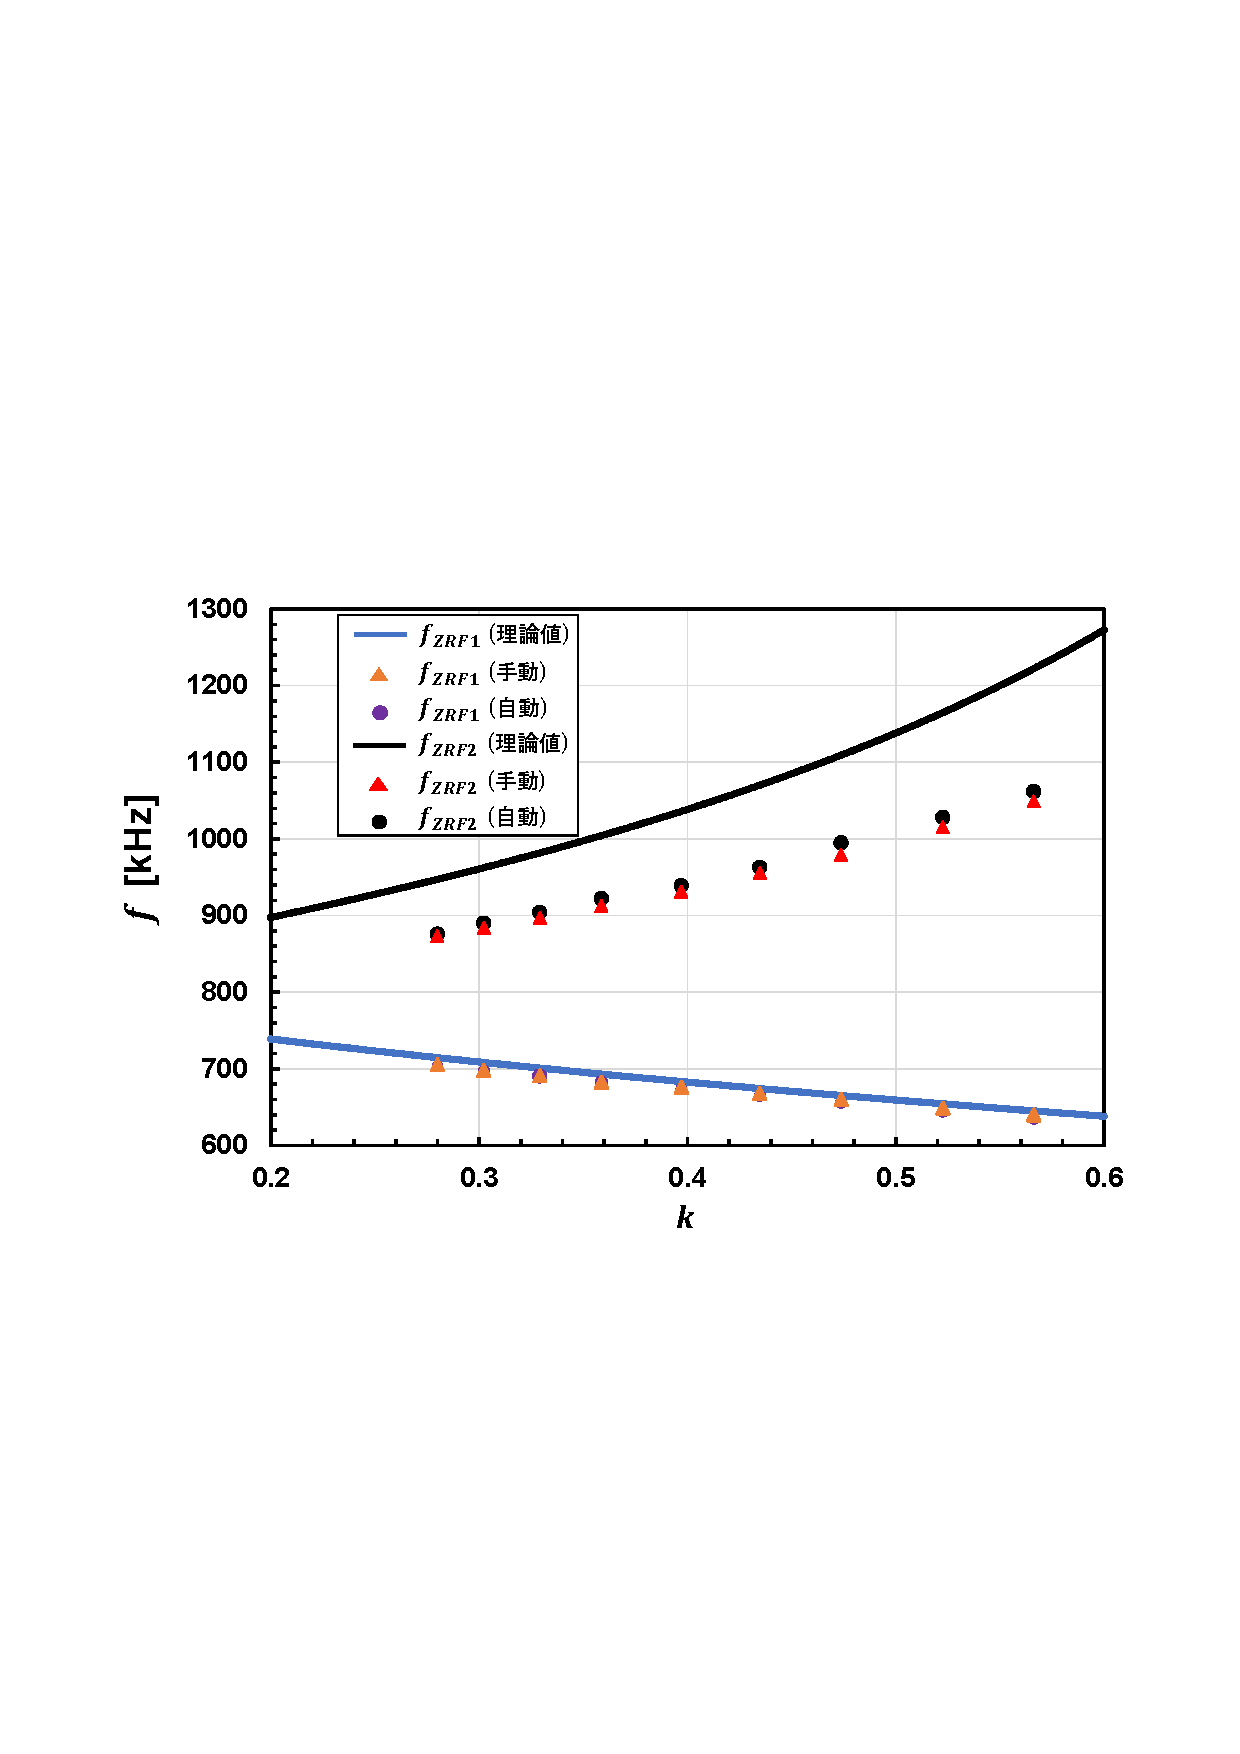
\includegraphics[width=140mm]{figures/tracking1.pdf}
\caption{ZRFの測定結果}
\label{tracking1}
\vspace{1cm}

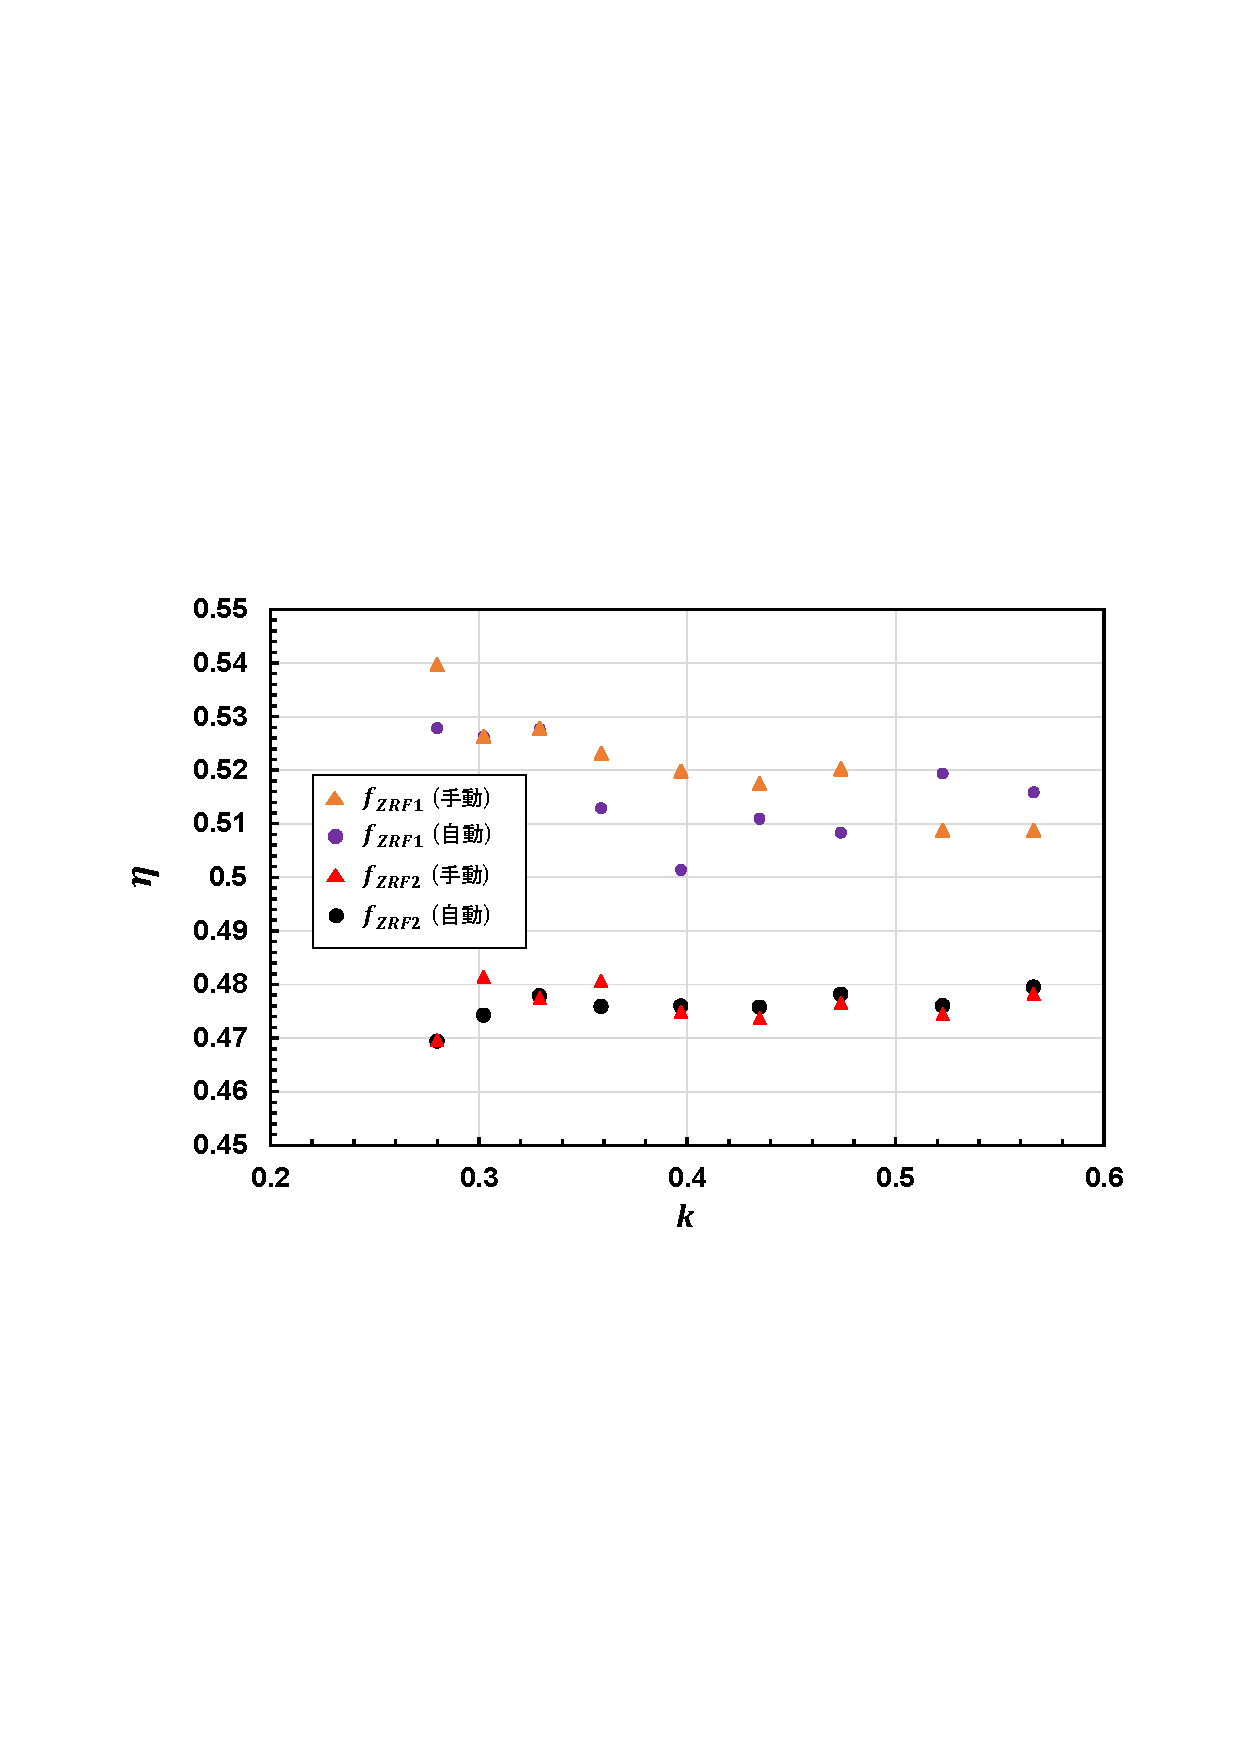
\includegraphics[width=140mm]{figures/tracking2.pdf}
\caption{電力効率の測定結果}
\label{tracking2}

\end{center}
\end{figure}

\subsubsection{データ伝送時の出力スペクトルの測定}
前項の実験により,データ入力を固定したときはZRFの追従動作が行えることが確認できた.次に,データとして矩形波信号を入力したときの出力スペクトルを測定することにより,どの程度のビットレートまで追従動作が行えるかを調査した.このときの測定系を図\ref{spectrum}に示す.また,測定の様子の写真を図\ref{spectrumphoto}に示す.実験手順は次のとおりである.

\begin{enumerate}
  \item コイル間距離$d =5 \, \mathrm{mm}$, ハーフブリッジの入力電圧$V_{in}=5 \, \mathrm{V}$とした.
  \item 送電基板のデータ入力端子に,データ信号として周波数$f_{DATA}=0.1 \, \mathrm{kHz}$の矩形波信号を入力し,そのときの出力電圧$v_{out}$のスペクトルをスペクトラムアナライザで観測した.
  \item スペクトラムアナライザのカーソル機能を用い,スペクトルに現れた2つのピーク周波数を$f_{ZRF1},f_{ZRF2}$として記録した.
  \item 周波数$f_{DATA}$を徐々に上げながら,同様の測定を行った.
  \item コイル間距離$d =10 \, \mathrm{mm}$として,以上の測定を繰り返した.
\end{enumerate}
図\ref{spectrumgraph} (a),(b)に,各コイル間距離における$f_{DATA}$と$f_{ZRF1},f_{ZRF2}$の測定結果を示す.同図において,プロットが無い箇所はピークが判別できず欠測したものである(欠測があるのは$20 \mathrm{kHz}$以上の測定点であるが,このときは$10 \mathrm{kHz}$ごとに測定している).なお参考として,$f_{DATA}=0.1 \, \mathrm{kHz}$,$d=10 \, \mathrm{mm}$のときのスペクトルを図\ref{spectrumimage}に示す.\par
図\ref{spectrumgraph}より,$d=10 \, \mathrm{mm}$のときは$80 \, \mathrm{kHz}$程度,$d=5 \, \mathrm{mm}$のときは$10 \, \mathrm{kHz}$程度までZRFの追従動作が行えていると考えられる.また,$d=5 \, \mathrm{mm}$のとき,$30-60 \, \mathrm{kHz}$で欠測したのち,より高い周波数では再びピークが観測される現象が確認された.

\begin{figure}[p]
\begin{center}

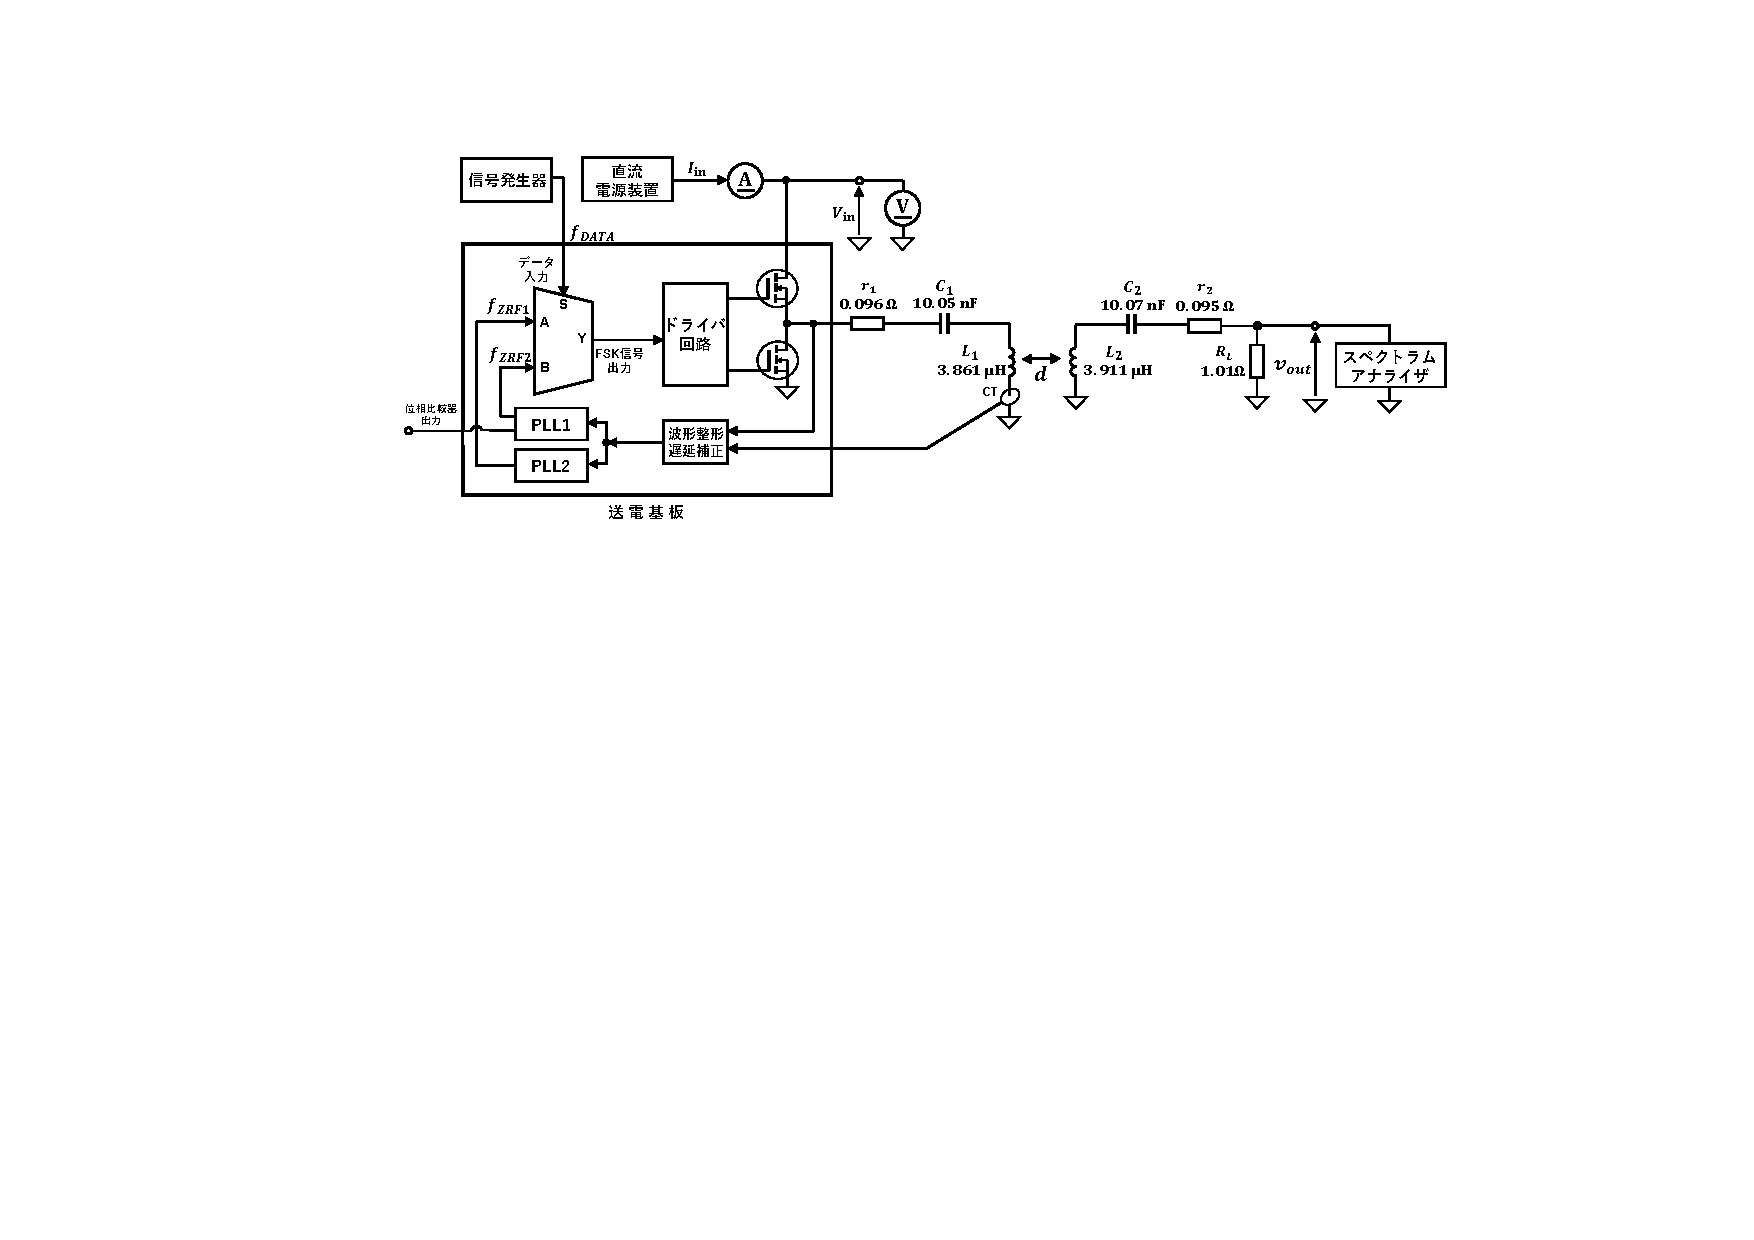
\includegraphics[width=160mm]{figures/spectrum.pdf}
  \caption{出力スペクトルの測定系}
  \label{spectrum}
\vspace{2cm}

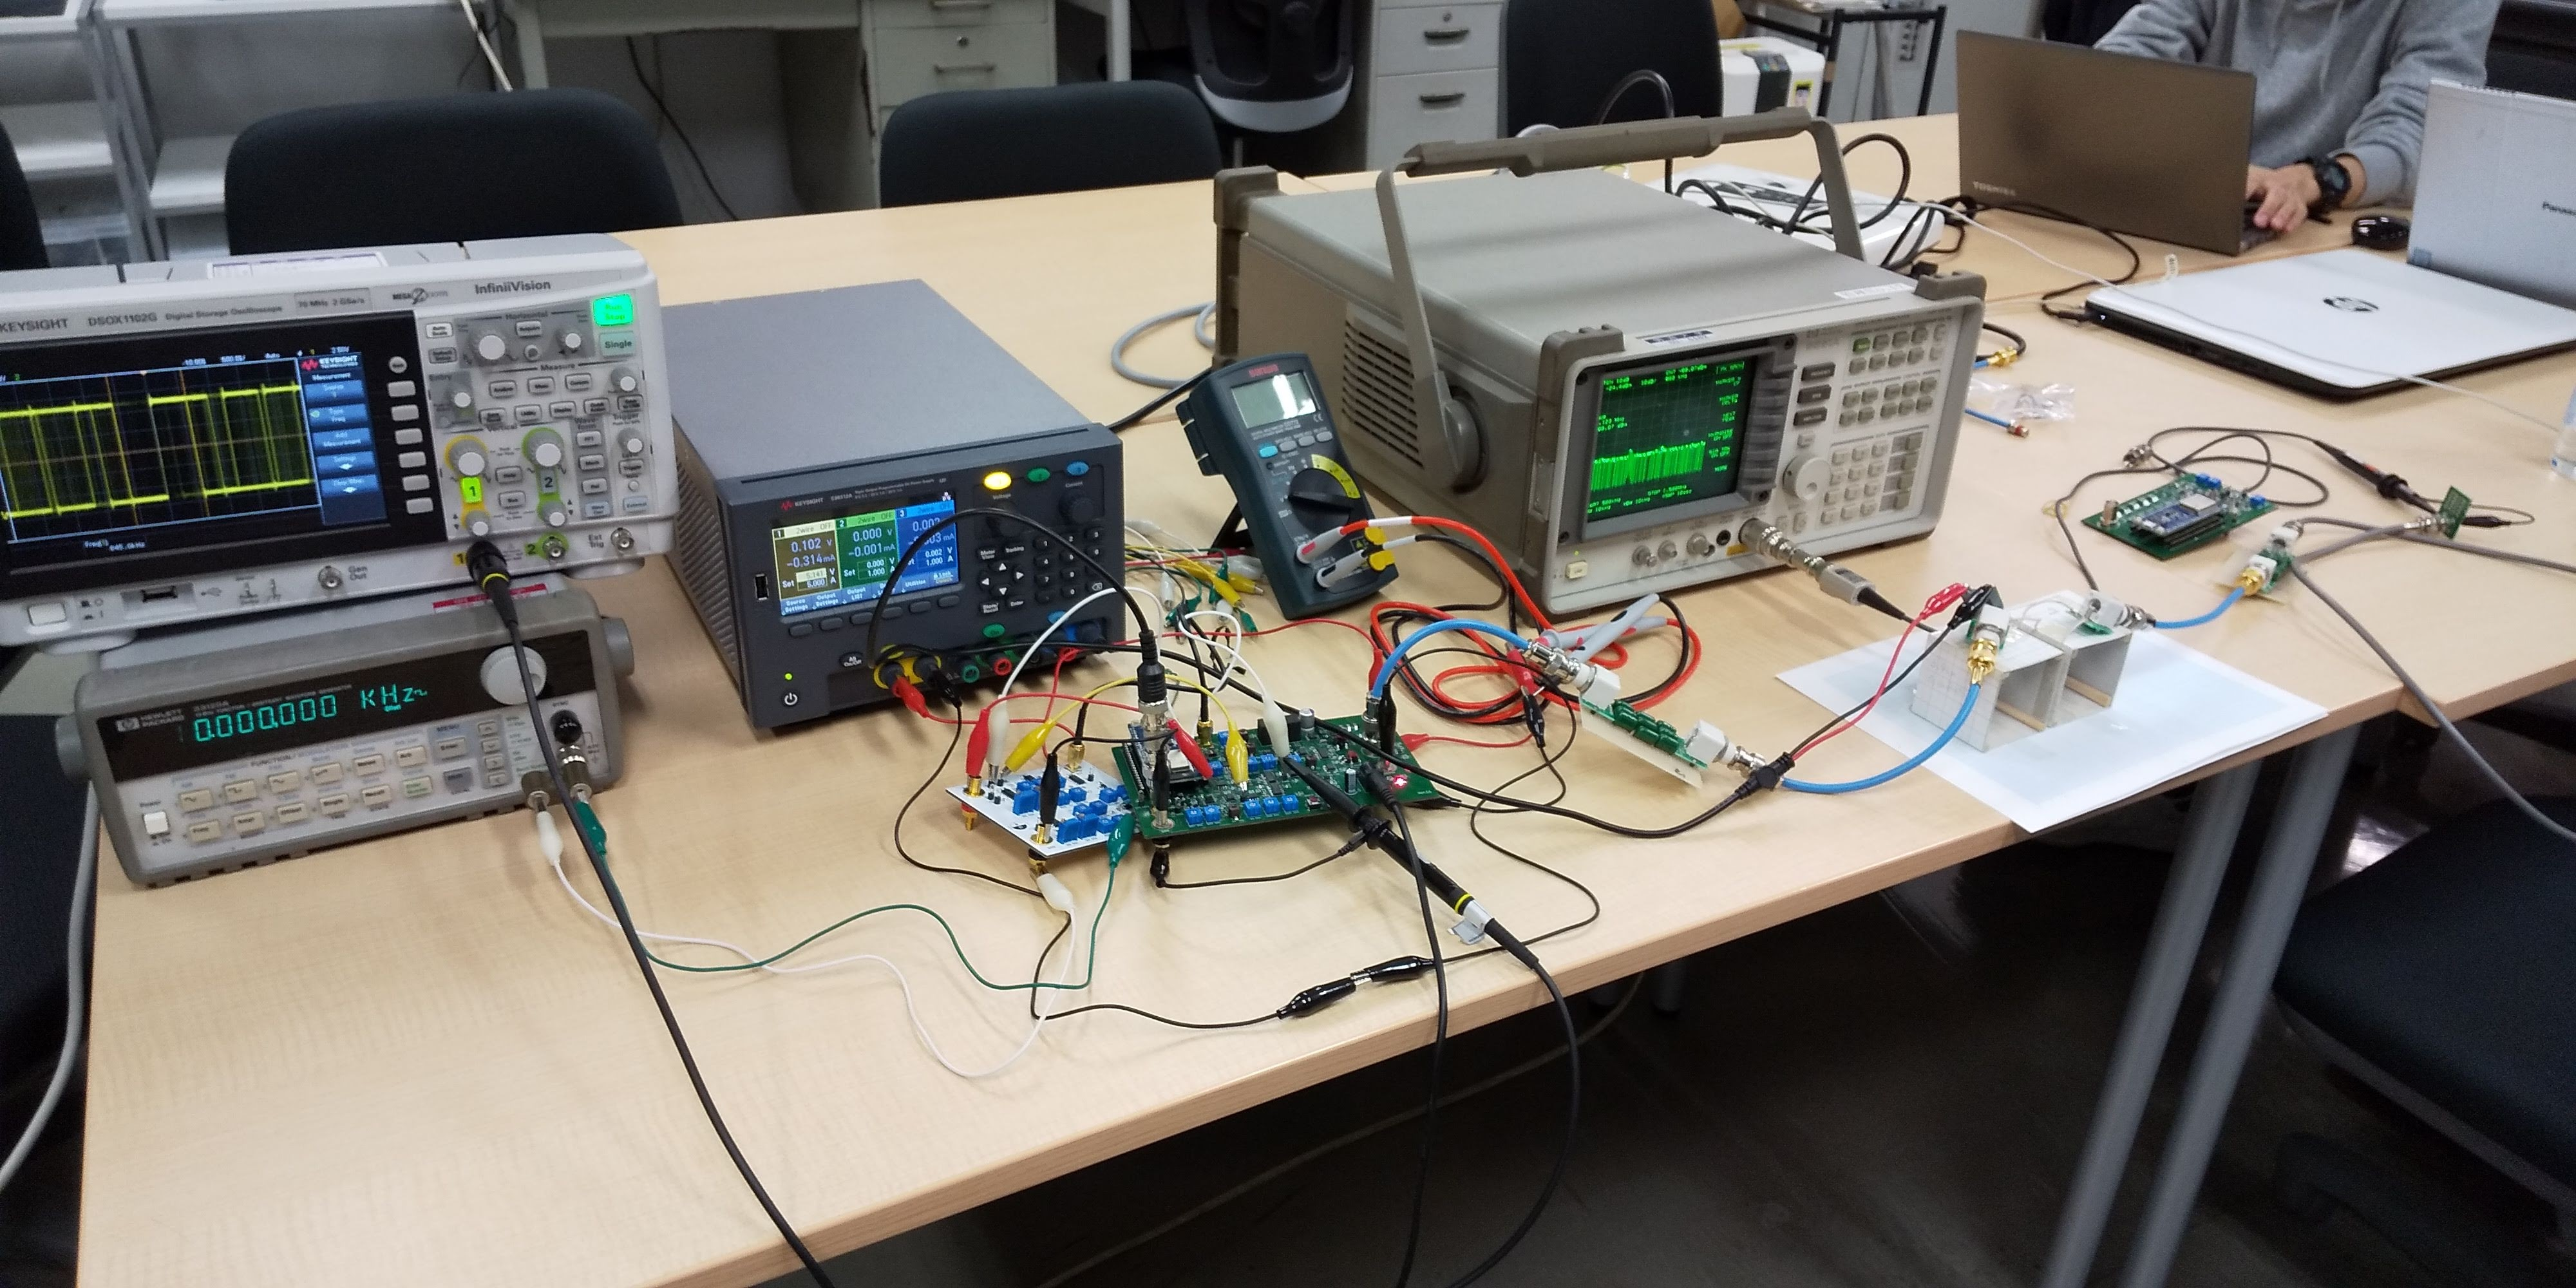
\includegraphics[width=160mm]{figures/spectrumphoto.jpg}
  \caption{出力スペクトルの測定風景}
  \label{spectrumphoto}
  \end{center}
\end{figure}

\begin{figure}[p]
\begin{center}

    \subfloat[$d= 5\, \mathrm{mm}$]{
    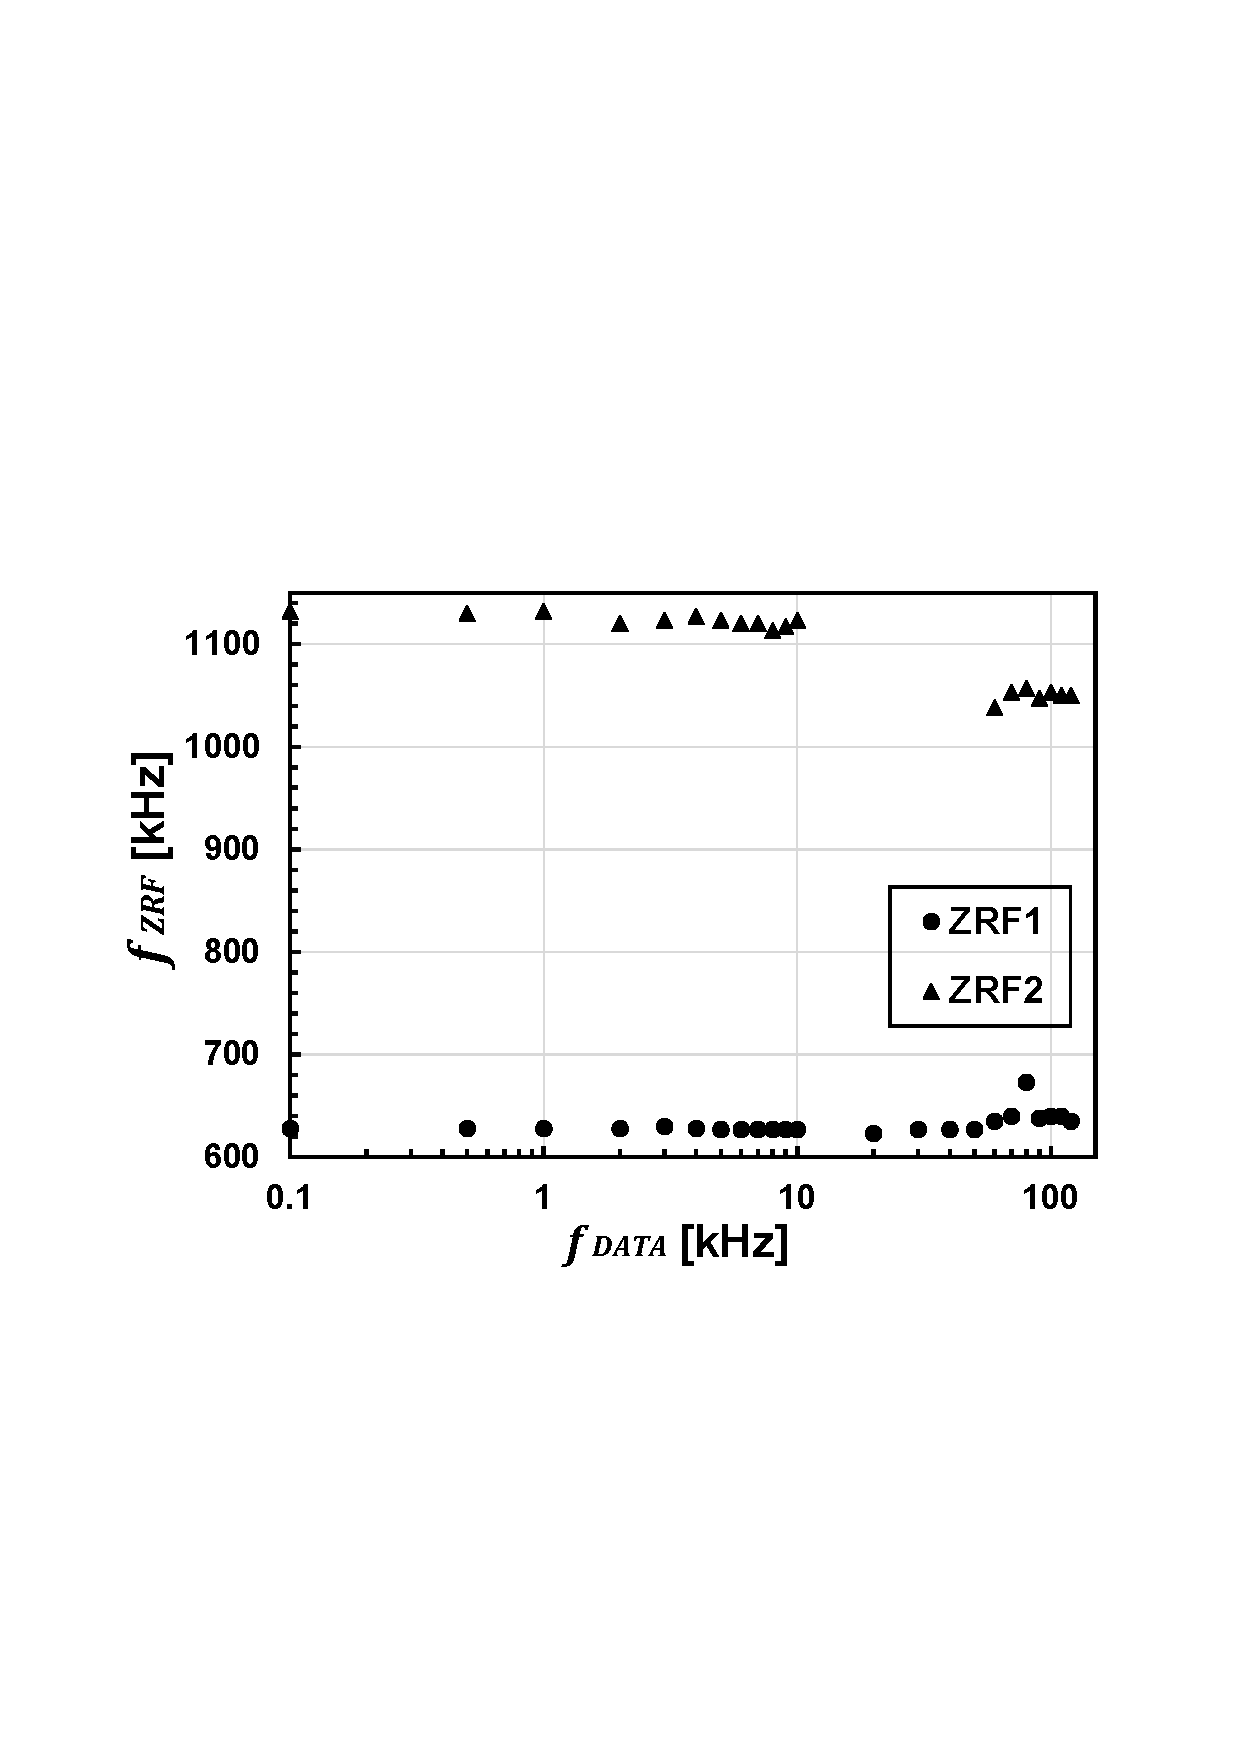
\includegraphics[width=75mm]{figures/spectrumgraph5.pdf}
    }    
    \subfloat[$d= 10\, \mathrm{mm}$]{
    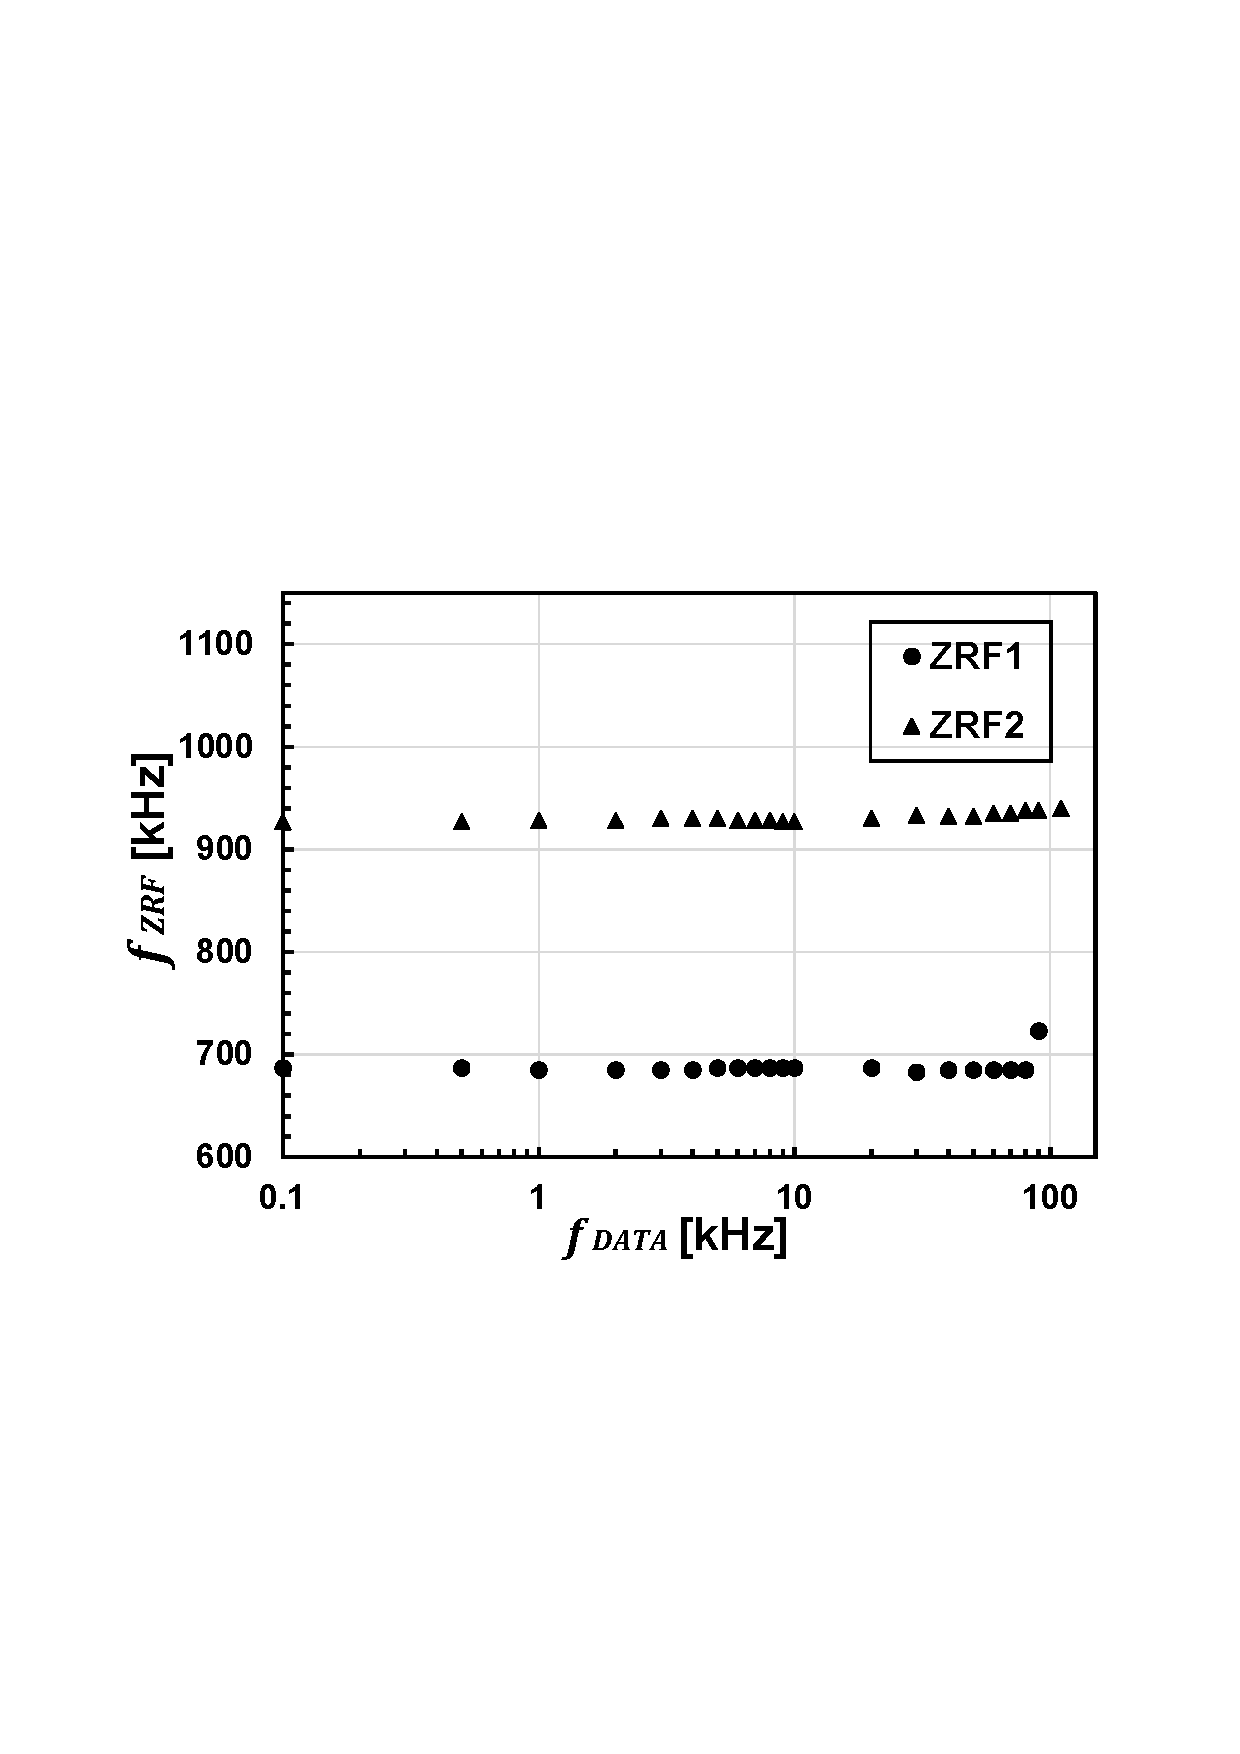
\includegraphics[width=75mm]{figures/spectrumgraph10.pdf}
    }
    
  \caption{出力スペクトルのピーク周波数の測定結果}\label{spectrumgraph}
  
  \vspace{2cm}
  
  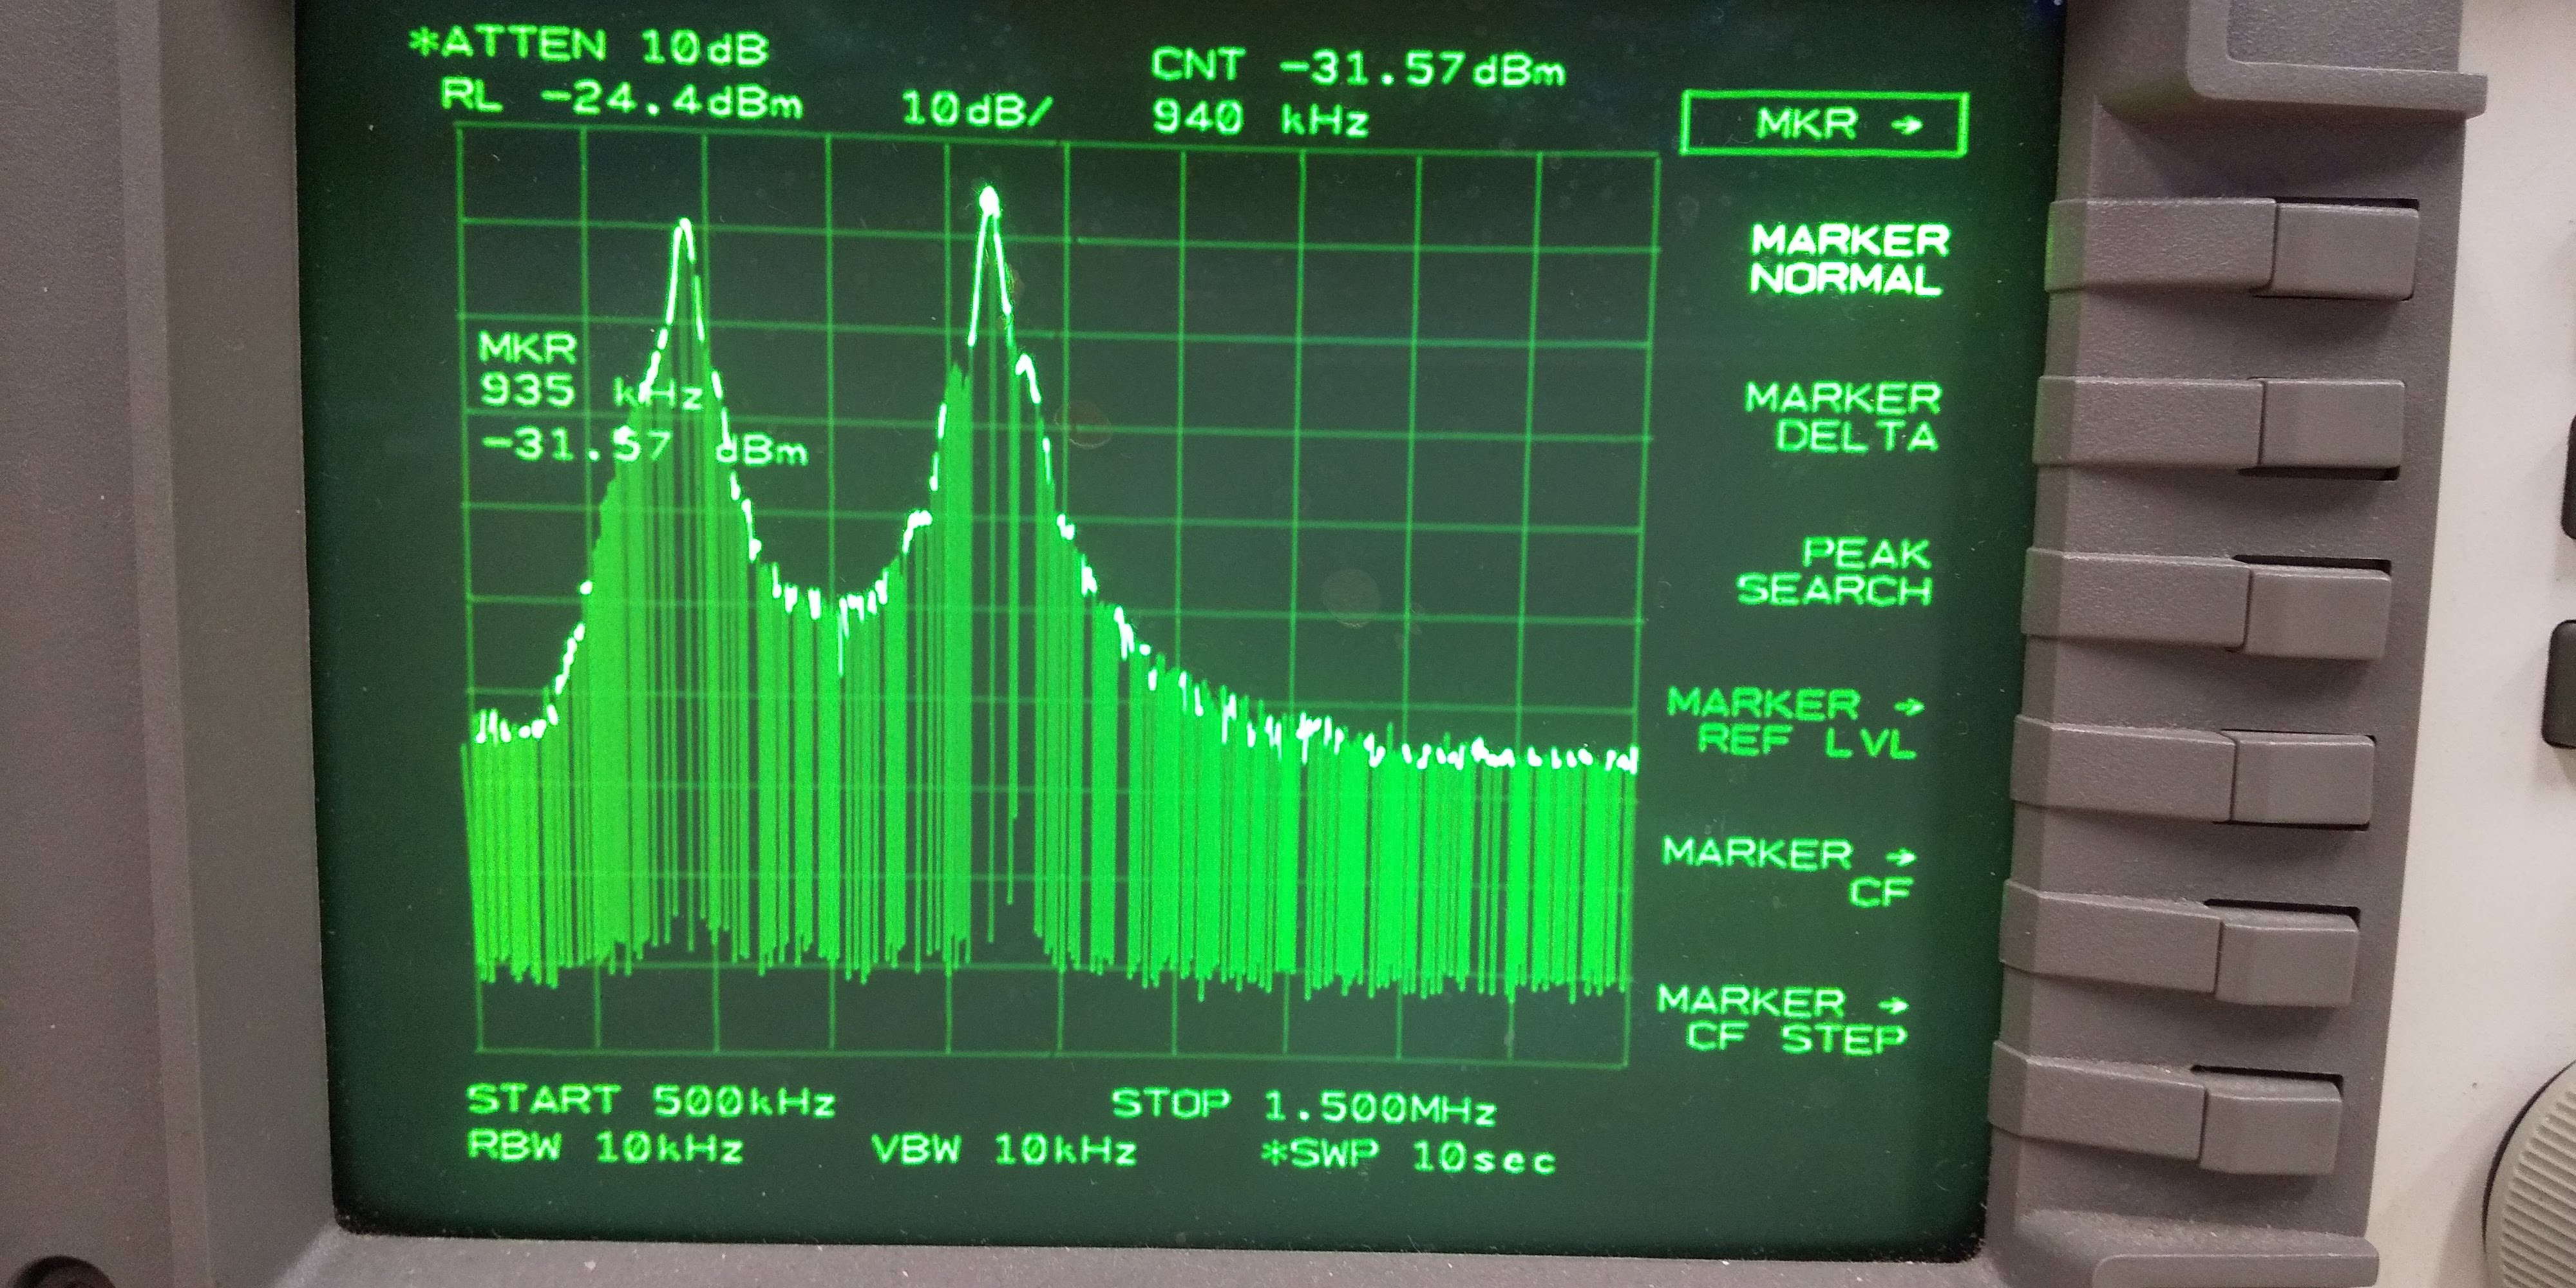
\includegraphics[width=160mm]{figures/spectrumimage.jpg}
  \caption{ $f_{DATA}=0.1 \, \mathrm{kHz}$,$d=10 \, \mathrm{mm}$のときの出力スペクトル}
  \label{spectrumimage}
  
  \end{center}
\end{figure}


\subsubsection{データ伝送速度-電力効率特性の測定}
データ伝送速度が電力効率に与える影響を調べる実験である.このときの測定系は,図\ref{spectrum}におけるスペクトラムアナライザを高周波電圧計に置き換えたものである.実験手順を以下に示す.

\begin{enumerate} \setlength{\itemsep}{-0.2cm}
  \item コイル間距離$d =5 \, \mathrm{mm}$, ハーフブリッジの入力電圧$V_{in}=5 \, \mathrm{V}$とした.
  \item 送電基板のデータ入力端子に,データ信号として周波数$f_{DATA}=0.1 \, \mathrm{kHz}$の矩形波信号を入力し,そのときの入力電流$I_{in}$ならびに出力電圧$v_{out}$を測定した.
  \item 式(4.8)により,電力効率$\eta$を求めた.
  \item 周波数$f_{DATA}$を徐々に上げながら,同様の測定を行った.
  \item コイル間距離$d =10 \, \mathrm{mm}$として,以上の測定を繰り返した.
\end{enumerate}
図\ref{datavseta} (a),(b)に,各コイル間距離における伝送速度-電力効率特性の測定結果を示す.なお,$f_{DATA}$を高くすると出力電圧が大きく振れ不安定になる現象が現れたため,$d =10 \, \mathrm{mm}$のときは$f_{DATA}=80 \, \mathrm{kHz}$,$d =5 \, \mathrm{mm}$のときは$f_{DATA}=10 \, \mathrm{kHz}$で,それぞれ測定を打ち切った.電力効率は,$f_{DATA}$に対してほぼフラットな特性,あるいは$f_{DATA}$が高くなるとともに上昇する現象が認められる.

\begin{figure}[h]
\begin{center}

    \subfloat[$d= 5\, \mathrm{mm}$]{
    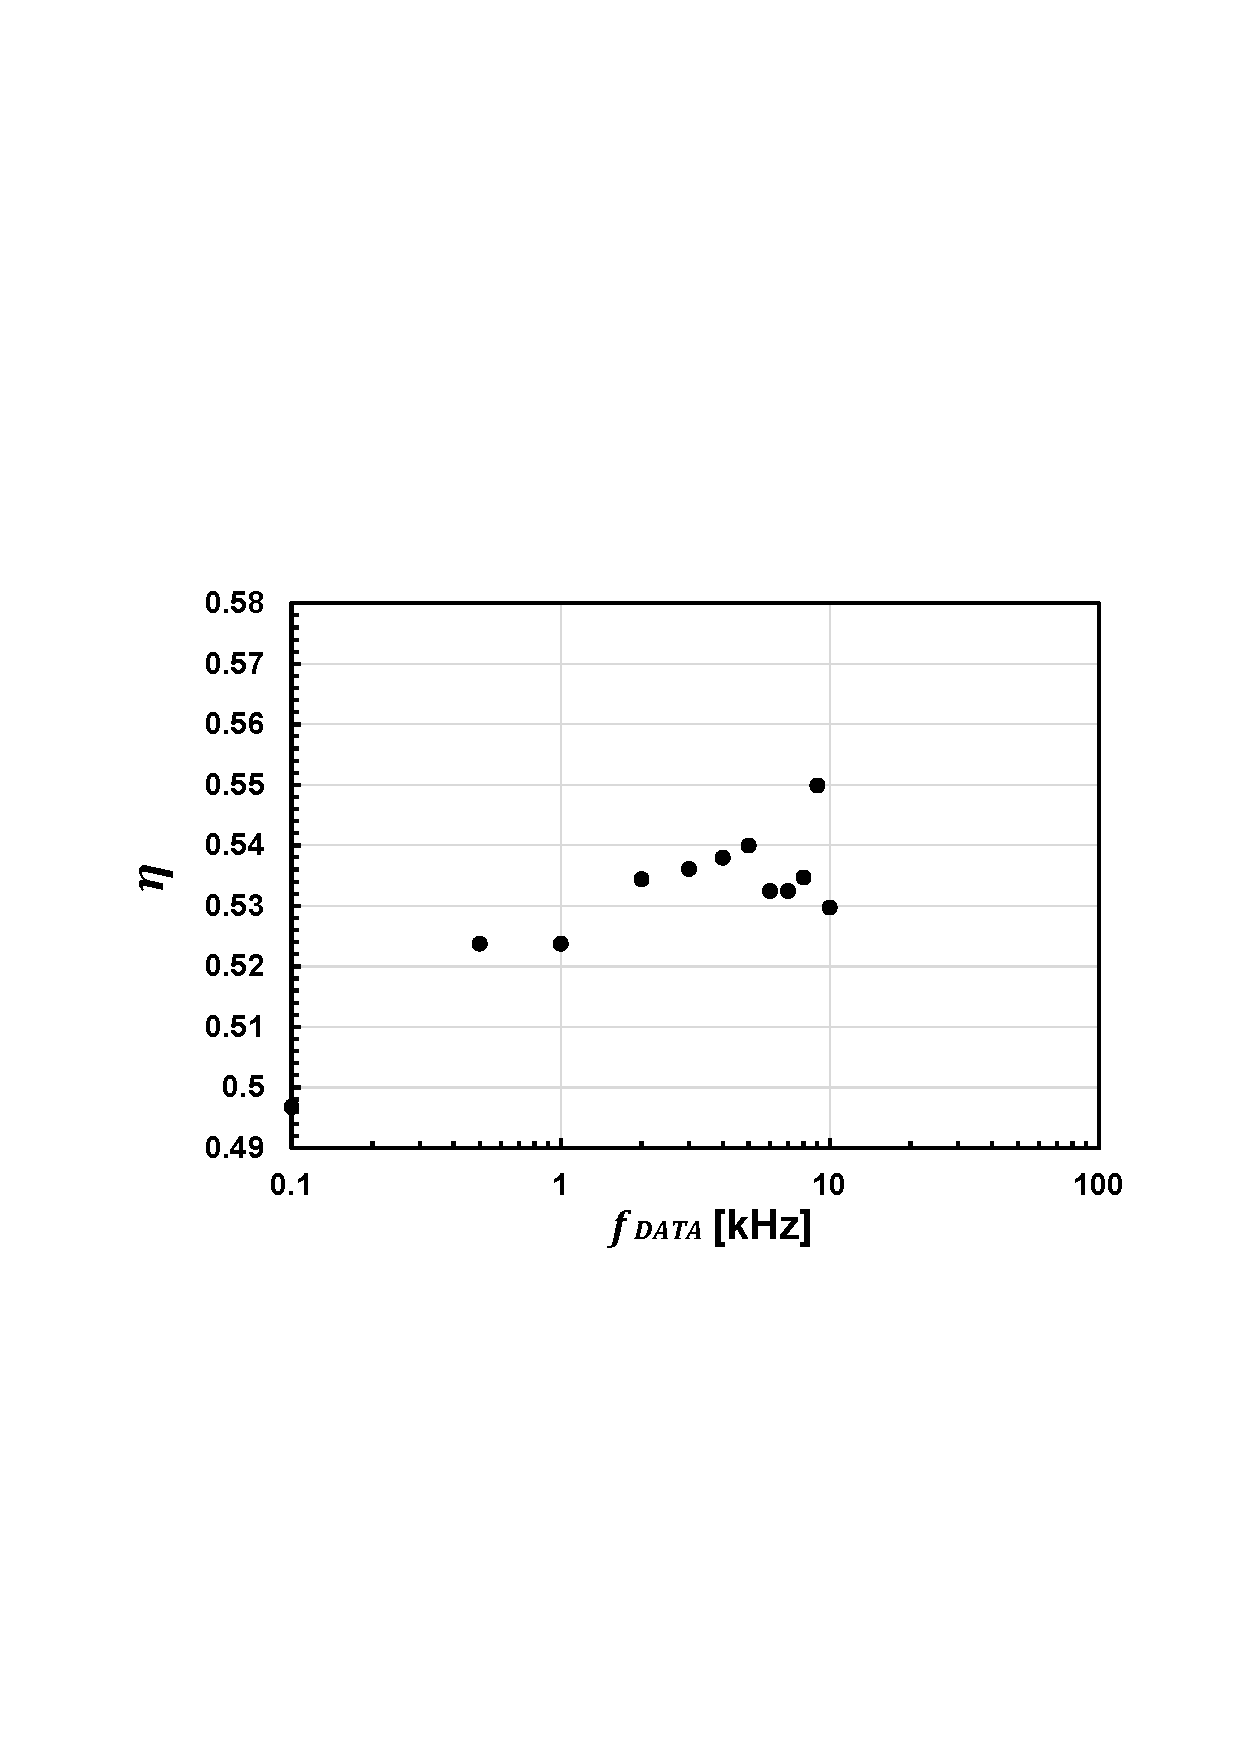
\includegraphics[width=75mm]{figures/datavseta5.pdf}
    }    
    \subfloat[$d= 10\, \mathrm{mm}$]{
    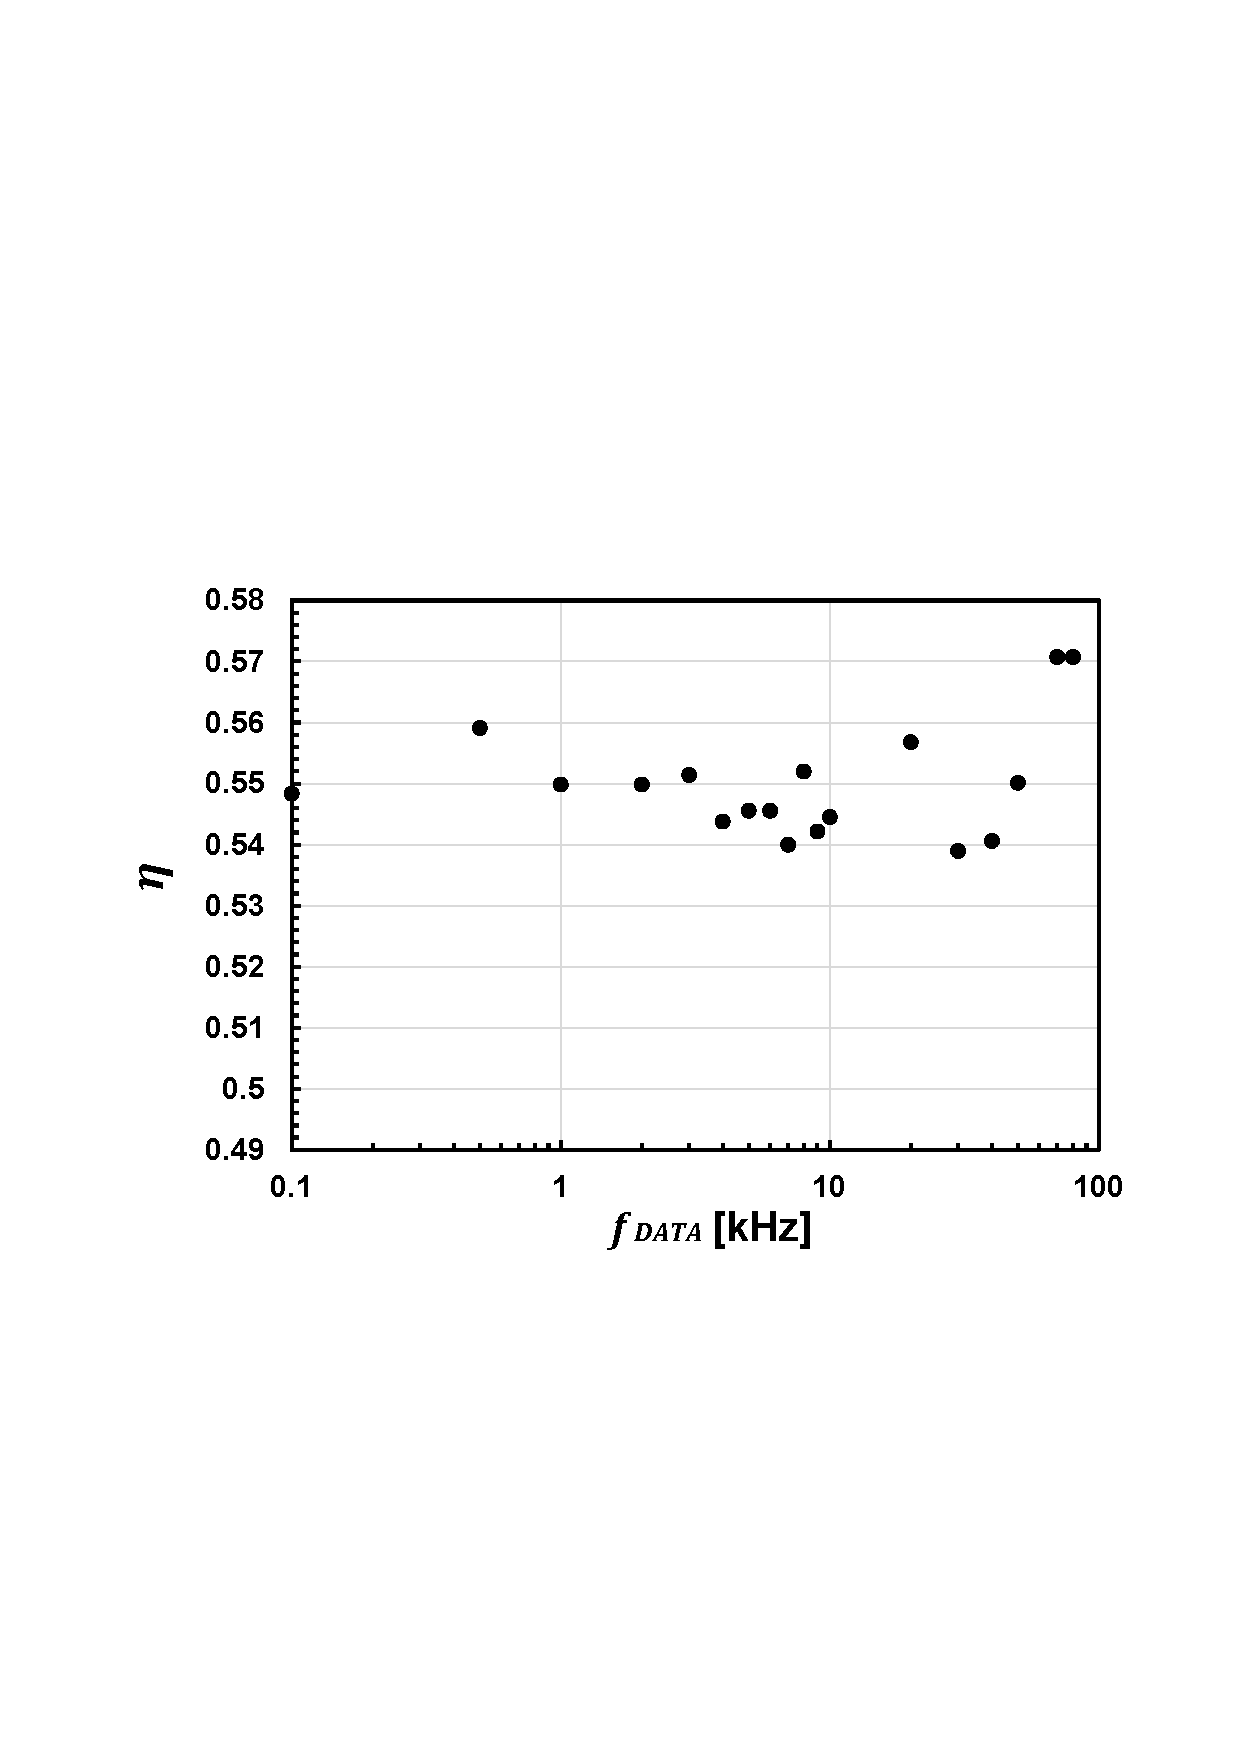
\includegraphics[width=75mm]{figures/datavseta10.pdf}
    }
     \caption{データ伝送速度-電力効率特性の測定結果}\label{datavseta} 
  \end{center}
\end{figure}


\subsubsection{文字列データ伝送実験}
送受信側にそれぞれPCを接続し,文字列を伝送する実験を行った.データの送受信には,PCのUSB端子と,Windows用のシリアル通信ソフトウェアTera Termを用いた.このときの実験系を図\ref{communication}に示す.なお,受信側回路の電源については,安定動作を図るために,PCのUSB端子から供給した.実験手順を以下に示す.

\begin{enumerate} \setlength{\itemsep}{-0.2cm}
  \item コイル間距離$d =10 \, \mathrm{mm}$, ハーフブリッジの入力電圧$V_{in}=5 \, \mathrm{V}$とした.
  \item 送電基板のデータ入力端子に,BER測定器からビットレート300 bpsの文字列データ信号を送信した.
  \item 受信側FPGAで復調したデータを,USB端子を経由してPC上のシリアルモニタに表示させ,文字列が正しく伝送されることを確認した.また,その際の直流出力電圧$V_{out}$ならびに入力電流$I_{in}$を測定し,電力伝送効率を求めた.
  \item ビットレートを徐々に上げながら,通信が不可能となるまで測定を行った.
  \end{enumerate}
送受信された文字列を目視で照らし合わせ確認したところ,ビットレート57.6 kbpsまでは誤り無く通信可能であった.このときの電力伝送効率は32.4\%であった.
\begin{figure}[h]
\begin{center}

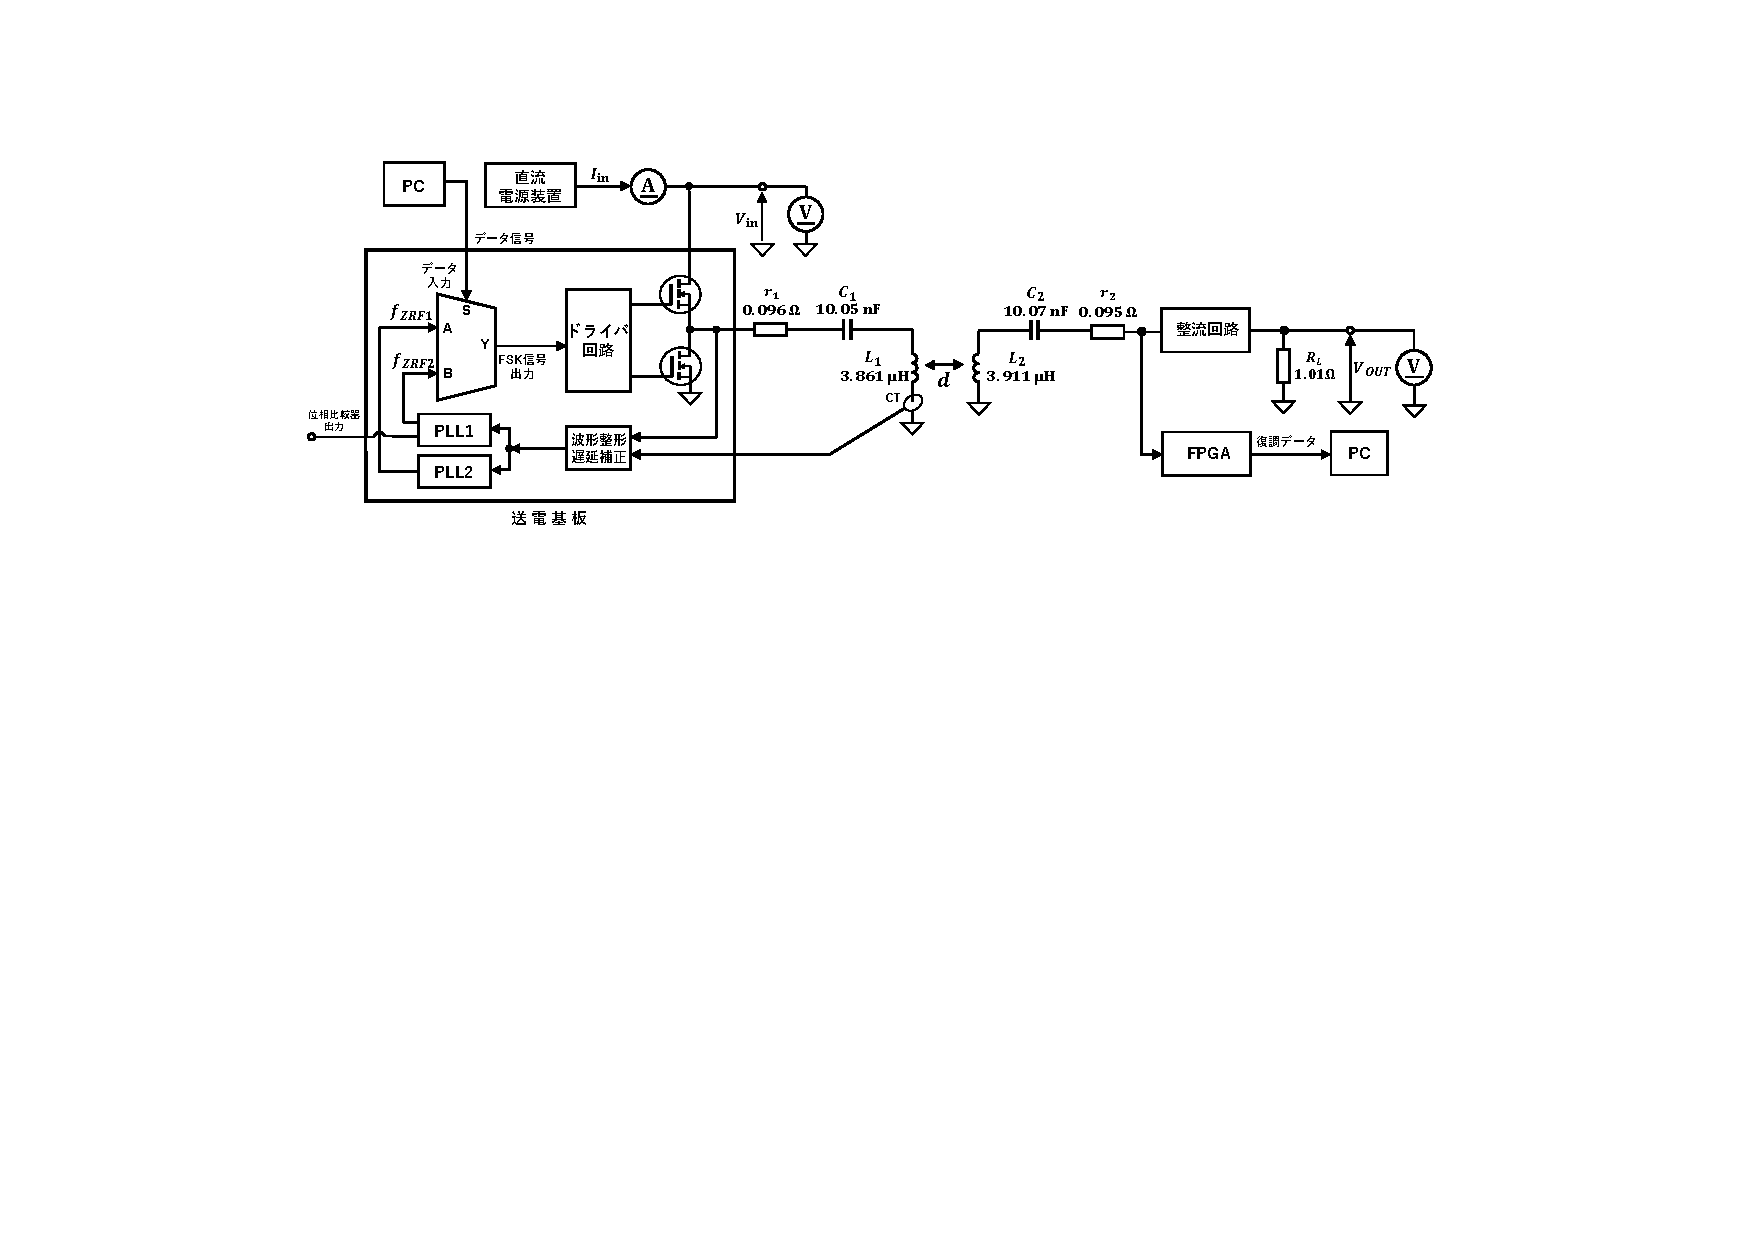
\includegraphics[width=160mm]{figures/communication.pdf}
  \caption{文字列データ伝送実験の測定系}
  \label{communication}

  \end{center}
\end{figure}


\subsubsection{BERの測定}
データの伝送特性をより定量的に把握するため,符号誤り率(Bit Error Rate : BER)の測定を行った.このときの実験系を図\ref{ber}に示す.実験手順は次のとおりである.
\begin{enumerate} %\setlength{\itemsep}{-0.2cm}
  \item コイル間距離$d =10 \, \mathrm{mm}$, ハーフブリッジの入力電圧$V_{in}=5 \, \mathrm{V}$とした.
  \item 変調基板のデータ入力端子に,BER測定器からビットレート57.6 kbps の擬似ランダム符号を送信した.擬似ランダム符号の繰り返し周期は$2^{15}-1$(PN15系列)とした.
  \item $10^7$ビットの送信が完了した後,受信側のBER測定器に表示されたBERを記録した.
  \item ビットレートを3 kbpsごと66.6 kbpsまで上げながら,同様の測定を行った.測定は3回行い,その平均値を結果とした.
  \item コイル間距離$d =5 \, \mathrm{mm}$,$15 \, \mathrm{mm}$として,同様の測定を行った.ただし,ここでは測定を1回のみとした.
  \end{enumerate}

\begin{figure}[h]
\begin{center}

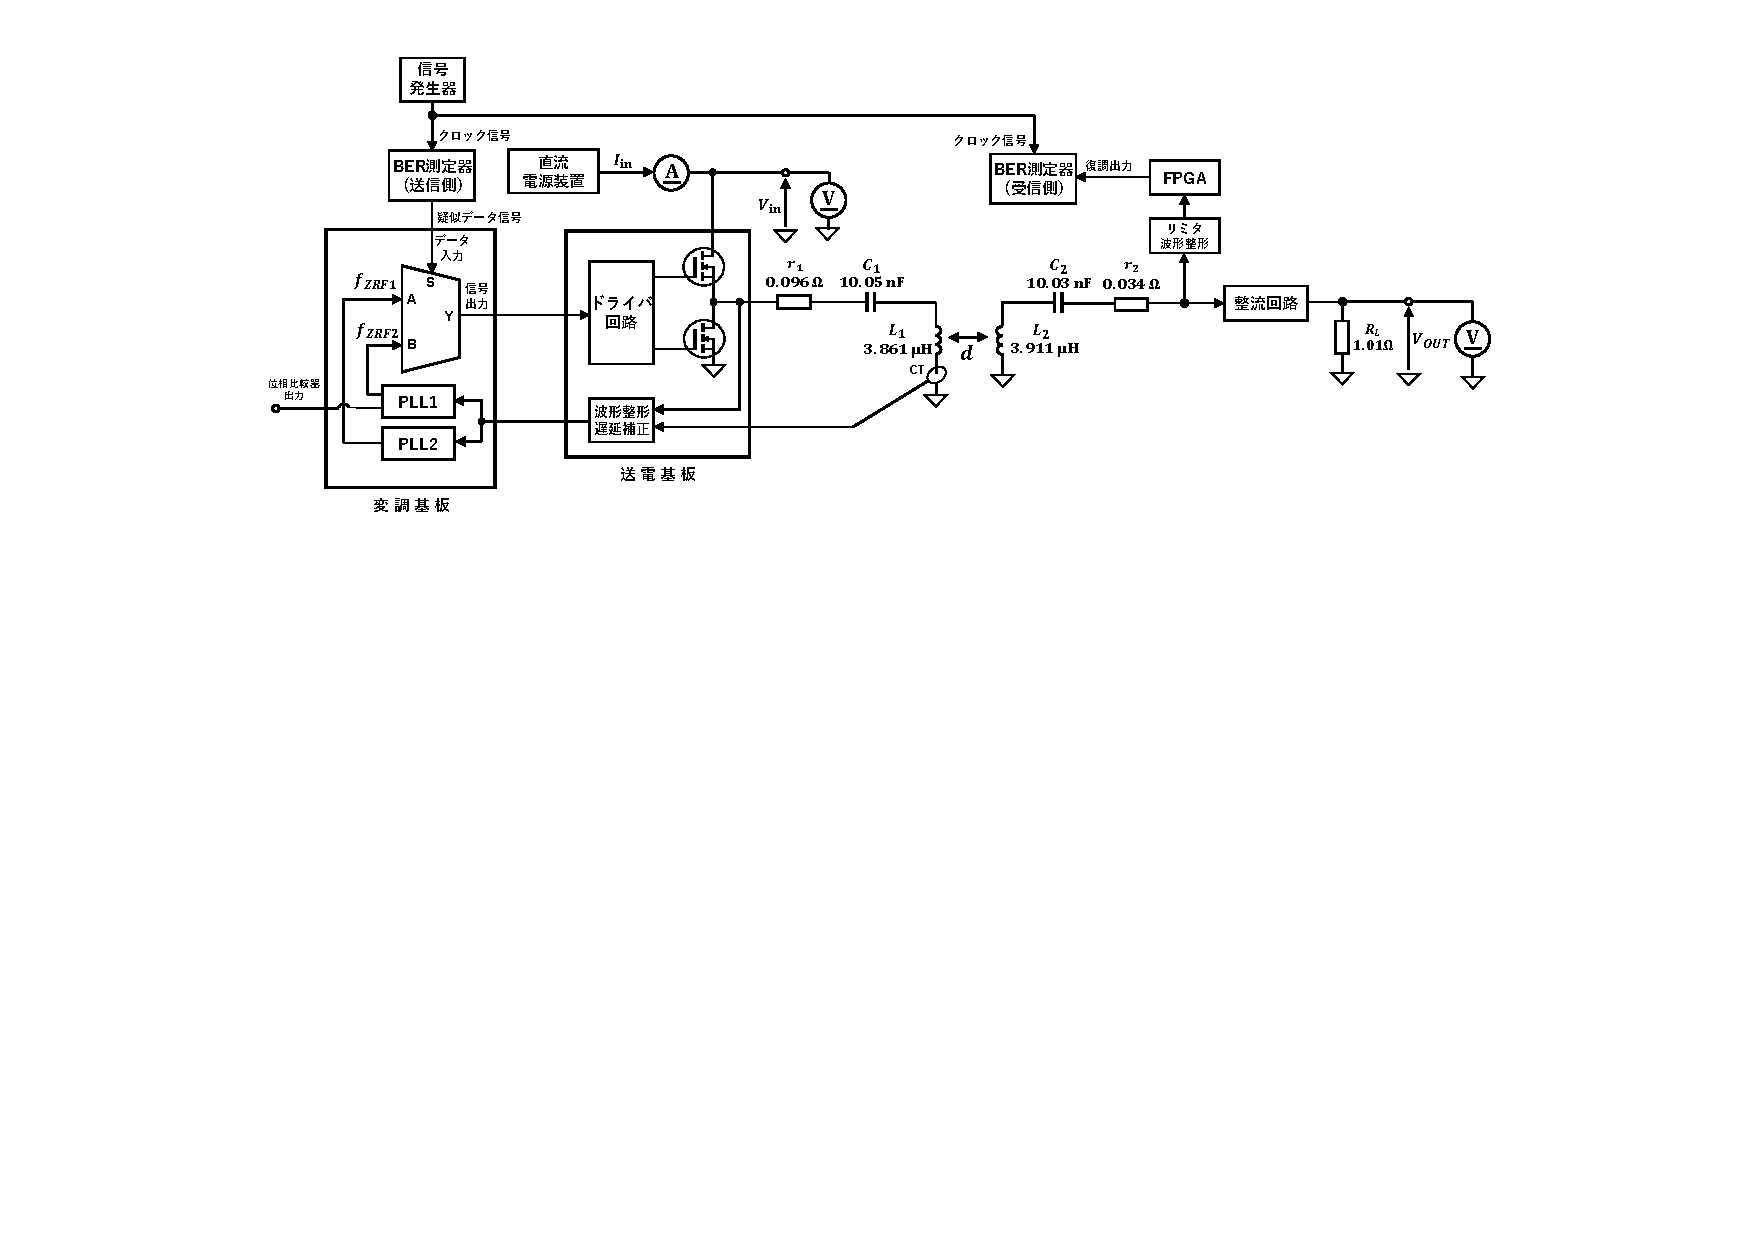
\includegraphics[width=160mm]{figures/ber.pdf}
  \caption{BERの測定系}
  \label{ber}

  \end{center}
\end{figure}

測定結果を図\ref{bergraph}に示す.同図の縦軸が対数軸であることに留意すれば,$d=1,1.5\, \mathrm{cm}$のとき,BERはビットレートに対して指数関数的に増大している.一方,$d=0.5\, \mathrm{cm}$では他の2つと異なり,ビットレートが低い場合でもBERが十分に小さくならない特性が認められる.

\begin{figure}[h]
\begin{center}

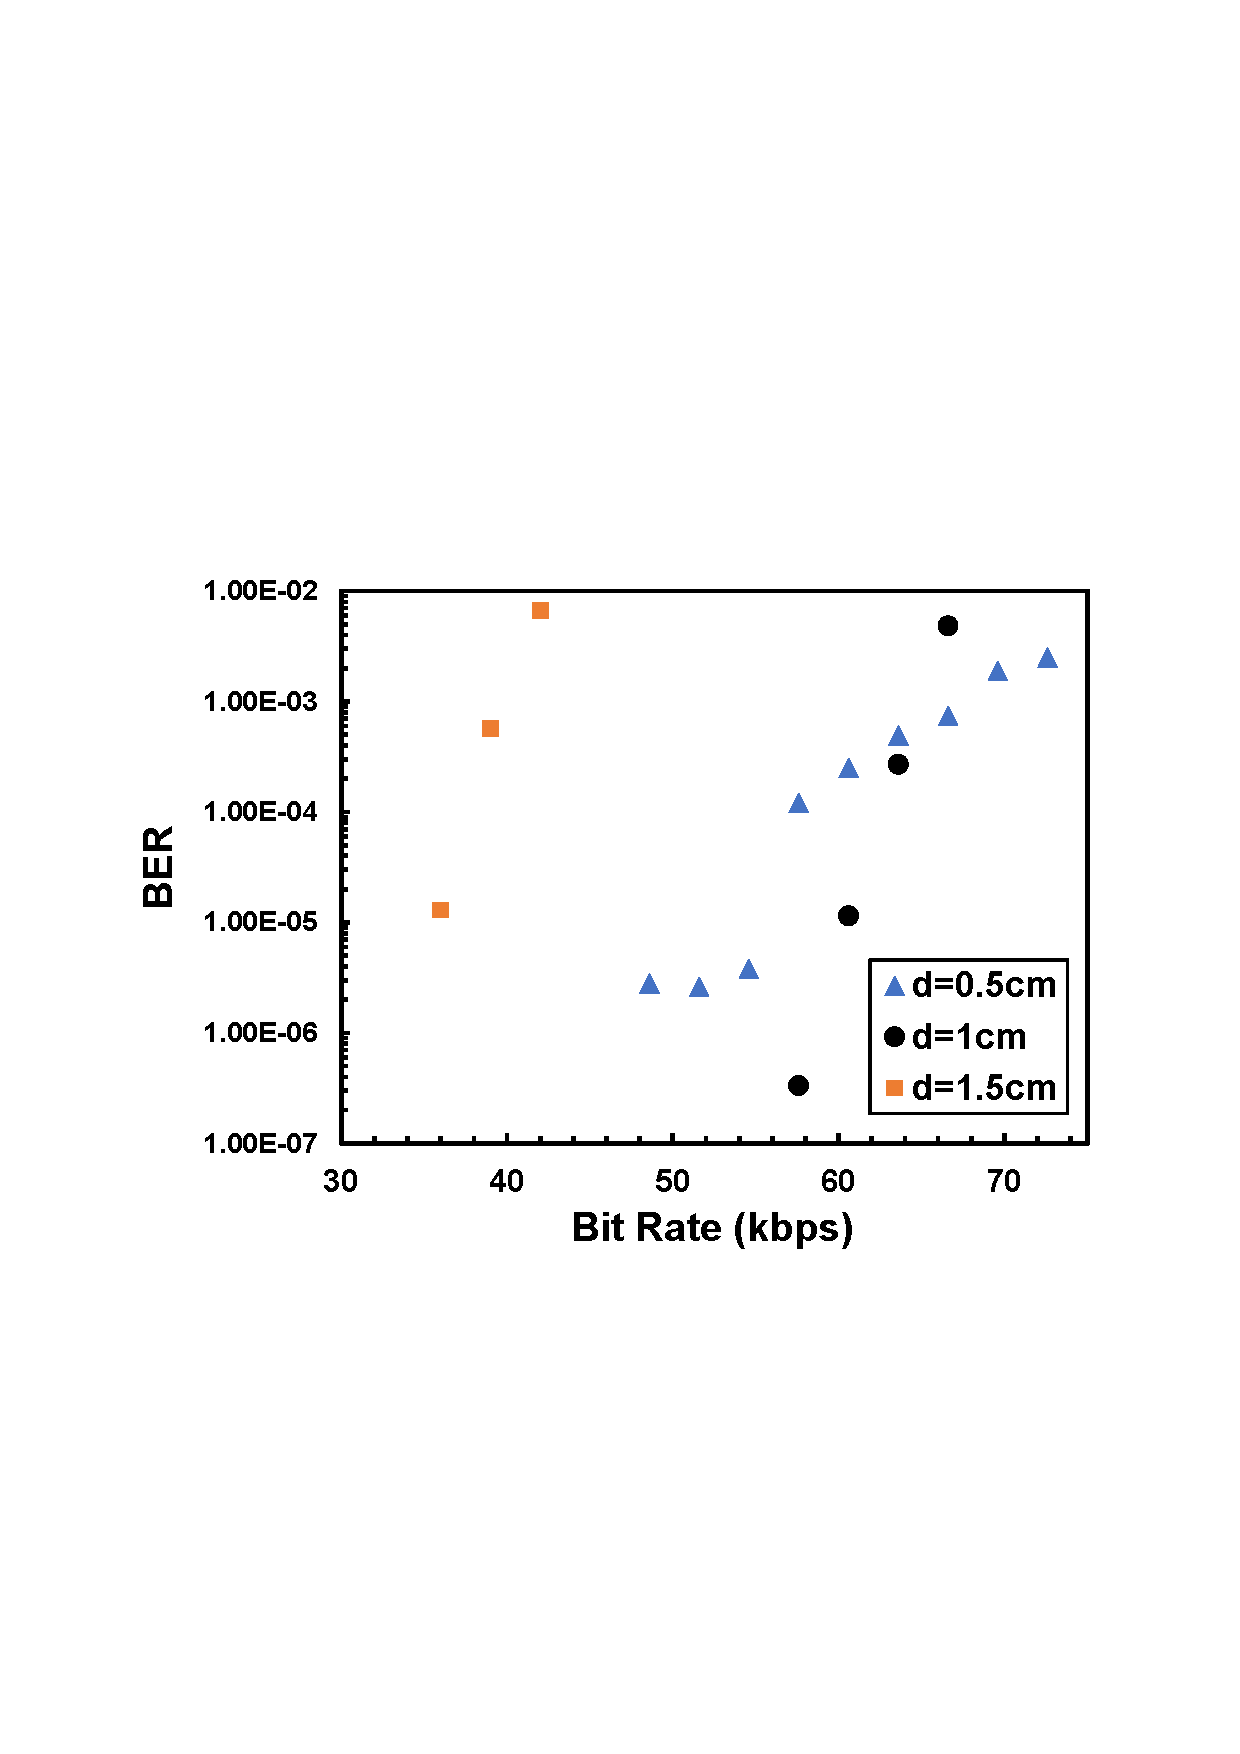
\includegraphics[width=120mm]{figures/bergraph.pdf}
  \caption{BERの測定結果}
  \label{bergraph}

  \end{center}
\end{figure}

